\documentclass%
%[handout]
{beamer}
% % % % % % % %
% % % % % % % %
% % % % % % % %
%IMPORTANT
%compiles with 
%pdflatex -shell-escape 
%IMPORTANT
% % % % % % % %
% % % % % % % %
% % % % % % % %
\mode<presentation>
{
\useinnertheme{rounded}
\useoutertheme{infolines}
\usecolortheme{orchid}
\usecolortheme{whale}
}

\usepackage[english]{babel}
\usepackage[latin1]{inputenc}
\usepackage[all,cmtip]{xy}
\usepackage{times}
\usepackage[T1]{fontenc}
\usepackage{../example-templates}
\usepackage{../pstricks-commands}

\usepackage{auto-pst-pdf}
\usepackage{pst-plot}
%\usepackage{pstricks-add} 

% Or whatever. Note that the encoding and the font should match. If T1
% does not look nice, try deleting the line with the fontenc.


\graphicspath{{../../modules/}}

\newtheoremstyle{partialproof}{3pt}{3pt}{}{}{}{.}{.5em}{}
\theoremstyle{partialproof} \newtheorem{partialproof}[theorem]{Proof.}
%\DeclareMathOperator{\diff}{d}
\setbeamertemplate{navigation symbols}{}

\includeonlylecture{1}

\newcommand{\lect}[3]{
  \date{#1}
  \lecture[#1]{#2}{#3}
}

\setbeamertemplate{footline}
{
  \leavevmode%
  \hbox{%
  \begin{beamercolorbox}[wd=.333333\paperwidth,ht=2.25ex,dp=1ex,center]{author in head/foot}%
    \usebeamerfont{author in head/foot}\insertshortauthor
  \end{beamercolorbox}%
  \begin{beamercolorbox}[wd=.333333\paperwidth,ht=2.25ex,dp=1ex,center]{title in head/foot}%
    \usebeamerfont{title in head/foot}\insertshorttitle
  \end{beamercolorbox}%
  \begin{beamercolorbox}[wd=.333333\paperwidth,ht=2.25ex,dp=1ex,center]{date in head/foot}%
    \usebeamerfont{date in head/foot}\insertshortdate{}
  \end{beamercolorbox}}%
  \vskip0pt%
}

% If you have a file called "university-logo-filename.xxx", where xxx
% is a graphic format that can be processed by latex or pdflatex,
% resp., then you can add a logo as follows:

%\pgfdeclareimage[height=0.8cm]{logo}{bluelogo}
%\logo{\pgfuseimage{logo}}
\renewcommand{\Arcsin}{\arcsin}
\renewcommand{\Arccos}{\arccos}
\renewcommand{\Arccot}{\text{arccot}}
\renewcommand{\Arctan}{\arctan}


\begin{document}

\AtBeginLecture{%

\title[\insertlecture]{FreeCalc}
\subtitle{\insertlecture}
\author[FreeCalc]{}
\institute[UMass Boston]{University of Massachusetts Boston}
\date{\insertshortlecture}
\begin{frame}
  \titlepage
\end{frame}
}%

% begin lecture
\lect{\today}{Sample}{1}
%\section{Integrals of form $\int R(x,\sqrt{ax^2+bx+c}) \diff x$, $R$ - rational function}
%%begin module Euler-substitution-intro
\begin{frame}
\frametitle{Integrals of form $\int R(x,\sqrt{ax^2+bx+c}) \diff x$, $R$ - rational function}
Let $R(x,y)$ be an arbitrary rational expression in two variables (quotient of polynomials in two variables).
\begin{question}
Can we integrate $\alert<10>{\displaystyle\int R(x,\sqrt{ax^2+bx+c})\diff x}$?
\end{question}
\begin{itemize}
\item<2-> Yes. We will learn how in what follows.
\item<3-> The algorithm for integration is roughly:
\begin{itemize}
\item<4-> Use linear substitution to transform to one of three integrals: 
\uncover<5->{$\int R(x, \sqrt{-x^2+1})\diff x$, } \uncover<6->{ $\int R(x, \sqrt{x^2+1})\diff x$, } \uncover<7->{$\int R(x, \sqrt{x^2-1}) \diff x$.}
\item<8-> Use Euler substitution to transform to rational function integral (no radicals).
\item<9-> Solve as previously studied.
\end{itemize}
\item<10,11-> We motivate why we need \alert<10>{such integrals later}; we promise they allow to compute ellipse area and the volume of a ball.
\end{itemize}

\end{frame}
%end module Euler-substitution-intro
%\subsection{Euler substitution}
%%begin module Euler substitution
\begin{frame}
\frametitle{Euler substitution}
\begin{itemize}
\item Using linear substitutions, radicals of form  $\sqrt{ay^2+by+c})$, $a\neq 0$, $b^2-4ac\neq 0$ can be transformed to (multiple of):
\begin{itemize}
\item $\sqrt{x^2+1}$ 
\item $\sqrt{-x^2+1}$
\item $\sqrt{x^2-1}$.
\end{itemize}
\item We already studied how to do that using completing the square. 
\end{itemize}
\end{frame}
\begin{frame}
Recall that a (real) linear substitution is a substitution of the form $u=px+q$, $p,q$- (real) constants.
\begin{example}
Use a linear substitution to transform $\sqrt{x^2+x+1}$ to a multiple of an expression of the form $\sqrt{u^2+1}$. 

\[
\begin{array}{rcl}
\sqrt{x^2+x+1}&=&\sqrt{ x^2+2\frac{1}{2}x +\frac{1}{4}\textbf{?}-\frac{1}{4}\textbf{?} +1} \\
&=& \sqrt{ \left(x+\frac{1}{2}\textbf{?} \right)^2-\textbf{?} }\\
&=&\sqrt{\frac{3}{4}\left( \frac{4}{3} \left(x+\frac{1}{2}\right)^2+1 \right)}\\
&=&\frac{\sqrt{3}}{2}\sqrt{\left(\frac{2}{\sqrt{3}}\left( x+\frac{1}{2}\right)\right)^2+1}\\
&=& \frac{\sqrt{3}}{2} \sqrt{u^2+1},
\end{array}
\]
where $u=\frac{2}{\sqrt{3}}\left( x+\frac{1}{2}\right) \textbf{?}=\frac{2\sqrt{3}}{3}x+\frac{\sqrt{3}}{3}$.
\end{example}
\vspace{5cm}
\end{frame}
\begin{frame}
Recall that a (real) linear substitution is a substitution of the form $u=px+q$, $p,q$- (real) constants.
\begin{example}
Use a linear substitution to transform $\sqrt{-2x^2+x+1}$ to a multiple of an expression of the form $\sqrt{-u^2+1}$. 

\[
\begin{array}{rcl}
\sqrt{-2x^2+x+1}&=&\sqrt{ -2\left(x^2-\frac{1}{2}x -\frac{1}{2}\right) } \\
&=& \sqrt{ -2\left(x^2-2\frac{1}{4}x +\frac{1}{16}-\frac{1}{16}-\frac{1}{2}\right) }\\
&=&\sqrt{-2\left(\left(x-\frac{1}{16}\right)^2-\frac{9}{16} \right)}\\
&=&\sqrt{\frac{9}{8}\left(-\frac{16}{9}\left(x-\frac{1}{16}\right)^2+1 \right)}\\
&=&\frac{3}{\sqrt{8}}\sqrt{-\left(\frac{4}{3}\left(x-\frac{1}{16}\right)\right)^2+1 }\\
&=&\frac{ 3}{\sqrt{8}} \sqrt{-u^2+1}
\end{array}
\]
where $u=\frac{4}{3}\left(x-\frac{1}{16}\right)  \textbf{?}=\frac{4}{3}x-\frac{1}{12}$.
\end{example}
\end{frame}
%end module Euler substitution.
%%begin module Euler-substitution-case-1
\begin{frame}
\frametitle{Euler substitution to handle $\sqrt{x^2+1} $}
\begin{itemize}
\item<1-> Suppose we want to integrate 
\[
\int R(x, \sqrt{x^2+1})\diff x\quad .
\]
\only<2-11>{
\item<2-> Substitute $\alert<11>{\sqrt{x^2+1}}= \alert<7>{x} +t \uncover<7->{=\alert<7>{ \frac12\left(\frac{1}{t}- t\right)}+t =\alert<11>{\frac12\left(\frac{1}{t}+ t\right)}} $\uncover<7->{.} 
\item<3-> How is this a substitution of $x$ via t?
\uncover<4->{ Square both sides: 
\[
\begin{array}{rcl}
x^2+1&=&x^2+2xt+t^2\\
\uncover<5->{2xt&=&1-t^2}\\
\uncover<6->{\alert<7,8,11>{x}&\alert<7,8,11>{=}& \alert<7,8,11>{ \frac12\left(\frac{1}{t}- t\right)}}
\end{array}
\]
}
\item<8-> Take differentials on both sides:
\[
\alert<8>{\alert<11>{ \diff x}=  \alert<9,10>{\frac12 \diff \left(\frac{1}{t}- t\right)}}  \uncover<9->{\alert<9,10,11>{=}} \only<9>{\alert<9>{\textbf{?}}} \uncover<10->{\alert<10,11>{ -\frac12\left(\frac{1}{t^2} +1\right) dt} } {~~~~~~~~~~~~~~~~~~~~~~~~~~~~~~~~~~~~~~~~~~~~~~~~~~~~~~~~~~~~~~~~~~}
\] 
}
\end{itemize}
\uncover<12->{
\begin{definition}
The Euler substitution for $\sqrt{x^2+1} $ is the substitution given by
\[
\begin{array}{rcl}
\displaystyle\alert<12>{\sqrt{x^2+1}}&\alert<12>{=}&\displaystyle \alert<12>{\frac12 \left(\frac1t +t\right)} \\
\displaystyle\alert<12>{x}&\alert<12>{=}&\displaystyle \alert<12>{ \frac12 \left(\frac{1}{t}- t\right)} \\
\displaystyle \alert<12>{\diff x}&\alert<12>{=}&\displaystyle \alert<12>{ -\frac12\left(\frac{1}{t^2}+1\right) dt}
\quad .
\end{array}
\]
\end{definition}
}
\vspace{10cm}
\end{frame}
%end module Euler-substitution-case-1
%%begin module Euler-substitution-case-2
\begin{frame}
\frametitle{Euler substitution to handle $\sqrt{-x^2+1} $}
\begin{itemize}
\item<1-> Suppose we want to integrate 
\[
\int R(x, \sqrt{-x^2+1})\diff x\quad .
\]
\only<2-15>{
\item<2-> Substitute $\alert<9,15>{\sqrt{-x^2+1}}=(1-\alert<11>{x})t  \uncover<11->{ =\left( 1 -\alert<11>{ \left(1-\frac{2}{ t^2+1} \right)} \right)t =\alert<15>{\frac{2t}{t^2+1}}}$. 
\item<3-> How is this a substitution of $x$ via t?
\uncover<4->{
\[
\begin{array}{rcll|l}
\sqrt{-x^2+1}&=&(1-x)t&&\text{square}\\
\uncover<5->{(1-x)(1+x)&=&(1-x)^2t^2&&\text{divide by }1-x}\\
\uncover<6->{1+x&=&(1-x)t^2}\\
\uncover<7->{xt^2+x &=&t^2-1}\\
\uncover<8->{x(t^2+1) &=&t^2-1 &&\text{divide by }t^2+1}\\
\uncover<9->{\alert<11,12,15>{x}&\alert<11,15>{=}& \frac{  t^2\uncover<10->{+1-1}-1}{t^2+1} \uncover<10->{ = \alert<11,12,15>{1 -\frac{2}{ t^2+1} }\quad .}}
\end{array}
\] 
\item<12-> 
\[
\alert<12,15>{\diff x =} \alert<12,13,14>{ \diff \left(1-\frac{2}{t^2+1}\right)} \uncover<13->{\alert<13,14,15>{=}}\only<13>{\alert<13>{\textbf{?}}} \uncover<14->{\alert<14,15>{ \frac{4t}{(1+t^2)^2}dt} \quad .}
 {~~~~~~~~~~~~~~~~~~~~~~~~~~~~~~~~~~~~~~~~~~~~~~~~~~~~}
\] 
}
}
\end{itemize}
\uncover<16->{
\begin{definition}
The Euler substitution for $\sqrt{-x^2+1}$ is the substitution given by:
\[
\begin{array}{rcl}
\displaystyle \alert<16>{\sqrt{-x^2+1}}&\alert<16>{=}& \displaystyle  \alert<16>{\frac{2t}{t^2+1}}\\
\displaystyle  \alert<16>{x}&\alert<16>{=}&\displaystyle  \alert<16>{1-\frac{2}{t^2+1}}\\
\displaystyle \alert<16>{\diff x }&\alert<16>{=} & \displaystyle  \alert<16>{\frac{4t}{(t^2+1)^2}dt }\quad .
\end{array}
\] 
\end{definition}
}
\vspace{5cm}
\end{frame}
%end module Euler-substitution-case-2
%%begin module Euler-substitution-case-3
\begin{frame}

\frametitle{Euler substitution to handle $\sqrt{x^2-1} $}

\begin{itemize}
\item<1-> Suppose we want to integrate 
\[
\int R(x, \sqrt{x^2-1})\diff x\quad .
\]
\only<1-14>{
\item<2-> Substitute $\alert<14>{\sqrt{x^2-1}=}(\alert<10>{x}-1)t\uncover<10->{= \left(\alert<10>{ 1+\frac{2}{t^2-1}} -1\right)t =\alert<14>{\frac{2t}{t^2-1}} .}$ 
\item<3-> How is this a substitution of $x$ via $t$? 
\[
\begin{array}{rcll|l}
\uncover<4->{\sqrt{x^2-1}&=&(x-1)t&&\text{square}}\\
\uncover<5->{(x-1)(x+1)  &=&(x-1)^2t^2&&  \text{divide by } x-1} \\
\uncover<6->{x+1 &=&(x-1)t^2}\\
\uncover<7->{x(t^2-1) &=&1+t^2}\\
\uncover<8->{\alert<10,11,14>{x}&\alert<10,11,14>{=}&\displaystyle \frac{t^2\uncover<9->{-1+1}+1}{t^2-1} \uncover<9->{=\alert<10,11, 14>{1+\frac{2}{t^2-1}}}}
\end{array}
\]
\item<11->
\[
\alert<11>{ \alert<14>{\diff x=} \alert<12,13>{\diff \left(1+\frac{2}{t^2-1} \right)}} \uncover<12->{\alert<12,13>{=}} \only<12>{\alert<12>{\textbf{?}}} \uncover<13->{\alert<13,14>{\frac{-4t}{(t^2-1)^2}\diff t} .} {~~~~~~~~~~~~~~~~~~~~~~~~~~~~~~~~~~~~~~~~~~~~~~~~}
\] 
}
\end{itemize}
\uncover<15->{
\begin{definition}
\[
\begin{array}{rcl}
\displaystyle \alert<15>{\sqrt{-x^2+1}}&\alert<15>{=}&\displaystyle \alert<15>{\frac{2t}{t^2-1} }\\
\displaystyle \alert<15>{x}&\alert<15>{=}&\displaystyle \alert<15>{ 1+\frac{2} {t^2-1} }\\
\displaystyle \alert<15>{\diff x}&\alert<15>{=}&\displaystyle \alert<15>{ \frac{-4t }{(t^2-1 )^2}dt }\quad .
\end{array}
\] 
\end{definition}
}
\vspace{5cm}
\end{frame}
%end module Euler-substitution-case-3
%%begin module Euler-substitution-theorem
\begin{frame}
\frametitle{Summary of Euler substitution}

\begin{theorem}
Let $R(z,w)$ be an arbitrary rational function in two variables. Every integral of the form $\int R(x, \sqrt{ax^2+bx+c}) \diff x$ can be integrated using square roots, rational functions, logarithms, the $\Arctan$ function, and their compositions.
\end{theorem}
\begin{proof}
\begin{itemize}
\item<1-> Using linear substitutions we transform to integral of the form
$\int R(x, \sqrt{x^2+1}) \diff x$, $\int R(x, \sqrt{-x^2+1}) \diff x$ or $\int R(x, \sqrt{x^2-1}) \diff x$\quad .
\item<2-> Using one of the substitutions $t=\sqrt{x^2+1}-x$, $t=\frac{\sqrt{-x^2+1}}{-x+1}$,  $t=\frac{\sqrt{x^2-1}}{x-1}$ the integral is transformed to the form $ \int \frac{P(t)}{Q(t)}\diff t$. 
\item<3-> That is a rational function integral and can be solved using rational functions, logarithms, and the $\Arctan $ function.
\item<4-> Substitution of $t$ via $x$ may introduce extra square root.
\end{itemize}
\end{proof}
\end{frame}
%end module Euler-substitution-theorem
%\section{Integrals of form $\int R(\cos x,\sin x) \diff x$, $R$ - rational function}
%%begin module trig-integrals-rationalizing-substitution
\begin{frame}
\frametitle{Integrals of the form $\int R(\cos \theta,\sin \theta) \diff \theta$, $R$}

Let $R$ be an arbitrary rational function in two variables (quotient of polynomials in two variables).
\begin{question}
Can we integrate $\int R(\cos \theta, \sin \theta)\diff \theta$?
\end{question}
\begin{itemize}
\item<2-> Yes. We will learn how in what follows.
\item<3-> The algorithm for integration is roughly:
\begin{itemize}
\item<4-> Apply the substitution $\theta=2\Arctan t$ to transform to integral of rational function.
\item<5-> Solve as previously studied.
\end{itemize}
\end{itemize}
\end{frame}

\begin{frame}
\frametitle{The rationalizing substitution $\theta= 2\Arctan t$}
\uncover<13->{
\noindent 
Let $R$- rational function in two variables. 
$\int R(\alert<14,21>{\cos \theta,\sin \theta} ) \alert<22>{\diff \theta} $
can be integrated via the  substitution $\alert<14,15,18,23, 26>{ \theta=2\arctan t} $.
\uncover<14->{ How does this transform \alert<14,21>{$\sin \theta$, $\cos\theta$}? }\uncover<22->{How does this transform $\alert<22>{\diff \theta} $?} \uncover<26->{\alert<26>{How is $t$ expressed via $\theta$?}}
\[
\begin{array}{rcl}
\uncover<14->{ \alert<14,21>{\sin\alert<15>{\theta}}} &\uncover<14->{=} &\displaystyle \uncover<15->{ \alert<16>{\sin (\alert<15>{ 2\Arctan t} )}} \uncover<16->{ \alert<16>{= \frac{2 \alert<17>{\tan\left( \Arctan t\right)} }{1 + {\alert<17>{\tan}}^2 \alert<17>{ \left(\Arctan t \right)}} }} \uncover<17->{\alert<21>{ = \frac{2\alert<17>{ t}}{1+ {\alert<17>{t }}^2}}}\\
\uncover<14->{\alert<14,21>{\cos \alert<18>{\theta}}  } &\uncover<14->{=} &\displaystyle \alert<19>{ \uncover<18-> {\alert<19>{ \cos (\alert<18>{2\Arctan t}) }} } \uncover<19->{ \alert<19>{= \frac{1-{\alert<20>{\tan} }^2 \alert<20>{ (\Arctan t)}}{1+ {\alert<20>{\tan}}^2 \alert<20>{ (\Arctan t) }}}} \uncover<20->{  \alert<21>{= \frac{1- {\alert<20>{ t}}^2 }{1 +{\alert<20>{t} }^2}}} \\
\only<22->{
\uncover<22->{
\alert<22,23>{\diff \theta}}&\uncover<23->{\alert<23>{=}}& \displaystyle \uncover<23->{ \alert<23,24,25>{2 \diff \left(\Arctan t\right)}}\uncover<24->{ \alert<24,25>{=  \uncover<25->{ \alert<25>{\frac{1}{ 1+t^2}}} \uncover<24->{ \uncover<24>{ \textbf{?}}} \diff t}}\\
\uncover<26->{\alert<26,27>{t}&\alert<26,27>{=}&}\displaystyle \uncover<27->{\alert<27>{\tan \left(\frac{\theta}{2}\right)} }
}
\end{array}
\]
}

\only<1-20>{
Recall the expression of $\sin (2z), \cos (2z)$ via $\tan z$:
\[
\begin{array}{rcl}
\uncover<1->{\alert<1,2,16>{\sin \left(2z\right)}} &\uncover<1->{\alert<1>{=}}&\displaystyle  \uncover<2->{ \alert<2>{2\sin z\cos z}} \uncover<3->{=\frac{2 \alert<5>{\sin z\cos z} \uncover<4->{\alert<4>{ \frac{1}{\alert<5>{ \cos^2z}}}}}{\alert<3,6>{( \cos^2z +\sin^2z) }\uncover<4->{\alert<4,6>{\frac{1}{\cos^2z}}}}} \uncover<5->{\alert<16>{= \frac{2\alert<5>{\tan z} }{ \alert<6>{ 1+ \tan^2z}} } \quad .}\\
\uncover<1->{\alert<7,8,19>{\cos (2z)} }& \uncover<7->{ \alert<7,8>{= }}&\displaystyle\uncover<8->{\alert<8>{ \cos^2z-\sin^2z}} \uncover<9->{= \frac{ \alert<11>{ \left(\cos^2 z-\sin^2 z\right) \uncover<10->{\alert<10>{ \frac{1}{ \cos^2z} }}}}{\alert<12>{ \alert<9>{\left(\cos^2z +\sin^2 z\right)} \uncover<10->{\alert<10>{ \frac{1}{ \cos^2z }}} }}} \uncover<11->{\alert<19>{ =\frac{\alert<11>{ 1-\tan^2 z} }{\alert<12>{1+\tan^2z}}} ~ .}
\end{array}
\]
}



\uncover<28->{ 
\begin{theorem}
The substitution given above  transforms $ \int R(\cos \theta, \sin\theta)\diff \theta$ to an integral of a rational function of $t$.
\end{theorem}
}
\vspace{10cm}
\end{frame}
%end module trig-integrals-rationalizing-substitution
%%begin module trig-integrals-rationalizing-substitution-ex1
\begin{frame}
\begin{example}
\uncover<2->{Let $\alert<2,25>{\theta=2\arctan t}$, \alert<4>{$\cos \theta=\frac{1-t^2}{1+t^2}$}, \alert<3>{$\sin \theta=\frac{2t}{1+t^2}$}}\uncover<22->{, $\alert<22,24>{z= \frac{3}{\sqrt{5}} \left(t + \frac{1}{3} \right)}$.} 
\[
\begin{array}{rcl}
\displaystyle \int \frac{\alert<2>{ \diff \theta} }{ 2\alert<3>{\sin \theta} -\alert<4>{ \cos \theta} +5}
\only<1-16>{
\uncover<2->{&=& \displaystyle \int \frac{\alert<2>{ 2\diff t} }{\alert<2>{\alert<6,7,9>{(\alert<8>{1}+\alert<5>{t^2})}} \left(\alert<7>{ 2 \alert<3>{\frac{2 t}{ t^2+1}} } \alert<6,9>{-} \alert<4>{ \frac{(\alert<9>{ 1} \alert<6>{- t^2}) }{\alert<6,9>{1+t^2}}}+\alert<5,8>{5}\right)}} \\
\uncover<5->{ &=&\displaystyle \int \frac{\alert<10>{2} \diff t}{ \alert<5,6>{ \alert<10>{6}t^2} +\alert<7>{ \alert<10>{4} t} +\alert<8,9,10> {4}}}\\
\uncover<10->{&=&\displaystyle  \int \frac{\diff t}{\alert<10,11>{3}t^2+\alert<10>{2}t+\alert<10>{2}}}\\
\uncover<11->{ \uncover<12>{\alert<12>{\text{(complete square)}}} &=&\displaystyle \int \frac{\diff t}{ \alert<11>{3}\left(\alert<13>{ t^2+ 2t\frac{ 1}{\alert<11>{3}}} \uncover<12->{\alert<12>{\alert<13>{+ \frac{1}{9}} \alert<14>{-\frac{1}{9}}}} \alert<14>{+ \frac{ 2}{ \alert<11>{3}}} \right)}} \\
\uncover<13->{ &=& \displaystyle \frac{1}{3}\int\frac{\diff t}{\alert<13>{ \left(t+\frac{1}{3}\right)^2} + \alert<14,15>{ \frac{ 5}{9}}}} \\
}
\uncover<15->{&\alert<16,17>{=}&\alert<16,17>{\displaystyle \alert<18>{\frac{1}{3}} \int \frac{\diff t }{ \alert<15,18>{\frac{5}{9}} \left( \alert<15,19>{\frac{9}{5}} \left(t+ \frac{1}{3} \right)^2 +\alert<15>{1} \right)}}} {~~~~~~~~~~~~~~~~~~~~~~~~~~~~~~~} {~~~~~~~~~~~~~~~}\\
\only<17->{
\uncover<18->{&=&\displaystyle \alert<18>{\frac{3}{5}}\int \frac{\uncover<20->{\alert<20>{ \frac{\sqrt{5}}{3}}} \diff \left( \alert<22>{ \uncover<20->{\alert<20>{\frac{3}{ \sqrt{5}}}}\left( t \uncover<21->{\alert<21>{+\frac{1}{3}}}\right)} \right) }{\left(\left(\alert<22>{ \alert<19>{ \frac{3}{ \sqrt{5}}} \left( t+\frac{1}{3}\right)}\right)^{\alert<19>{2} }+1 \right)} }\\
\uncover<22->{ &=&\displaystyle \frac{\sqrt{5}}{5} \alert<23>{\int \frac{\diff \alert<22>{ z}}{{\alert<22>{ z}}^2+1}}}\\
\uncover<23->{&=& \displaystyle  \frac{\sqrt{5}}{5} \alert<23>{\Arctan \alert<24>{z}} +C} \\
\uncover<24->{ &=&\displaystyle \frac{ \sqrt{5}}{5}\Arctan \left(\alert<24>{ \frac{3}{ \sqrt{5}} \left(\alert<25>{ t}+\frac{1}{3} \right)} \right)+C}\\
\uncover<25->{&=&\displaystyle \frac{ \sqrt{5}}{5}\Arctan \left( \frac{3}{ \sqrt{5}} \left(\alert<25>{ \tan \left(\frac{\theta}{2} \right)}+\frac{1}{3} \right) \right)+C
}
}
\end{array}
\]

\end{example}
\vspace{5cm}

\end{frame}
%end module trig-integrals-rationalizing-substitution-ex1
%%begin module Euler-substitution-intro
\begin{frame}
\frametitle{Integrals of form $\int R(x,\sqrt{ax^2+bx+c}) \diff x$, $R$ - rational function}
Let $R(x,y)$ be an arbitrary rational expression in two variables (quotient of polynomials in two variables).
\begin{question}
Can we integrate $\alertNoH{10}{\displaystyle\int R\left(x,\sqrt{ax^2+bx+c} \right) \diff x}$?
\end{question}
\begin{itemize}
\item<2-> Yes. We will learn how in what follows.
\item<3-> The algorithm for integration is roughly:
\begin{itemize}
\item<4-> Use linear substitution to transform to one of three integrals:
\uncover<5->{$\int R(x, \sqrt{x^2+1})\diff x$, } \uncover<6->{$\int R(x, \sqrt{-x^2+1})\diff x$, } \uncover<7->{$\int R(x, \sqrt{x^2-1}) \diff x$.}
\item<8-> Use trigonometric substitution or Euler substitution to transform to trigonometric or rational function integral (no radicals).
\item<9-> Solve as previously studied.
\end{itemize}
\item<10-> We motivate why we need \alertNoH{10}{such integrals } by examples such as computing the area of an ellipse.
\end{itemize}
\end{frame}
%end module Euler-substitution-intro

%% begin module trig-substitutions-intro
\begin{frame}
\frametitle{Trigonometric Substitution}
\begin{itemize}
\item  To find the area of a circle or ellipse, one needs to compute $\int \sqrt{a^2 - x^2} \diff x$.
\item<2->  For $\int x\sqrt{a^2 - x^2}\diff x$, the substitution $u = a^2 - x^2$ would work.
\item<3->  For $\int \sqrt{a^2 - x^2}\diff x$, we need a more elaborate substitution.
\item<4-| alert@6>  Instead, substitute $x = a\sin \theta$.
\end{itemize}
\[
\uncover<5->{%
\sqrt{a^2-\alert<handout:0| 6>{x^2}} = %
}%
\uncover<6->{%
\sqrt{a^2-\alert<handout:0| 6>{a^2\sin^2 \theta}} = %
}%
\uncover<7->{%
\sqrt{a^2(1 - \sin^2 \theta )} = %
}%
\uncover<8->{%
\sqrt{a^2\cos^2 \theta} = a|\cos \theta |.%
}%
\]
\begin{itemize}
\item<9->  With $u = a^2 - x^2$, the new variable is a function of the old one.
\item<10->  With $x = a\sin \theta$, the old variable is a function of the new one.
%Greg: the below remarks seem redundant to me. Students know how to compute \diff x, I'd think they'd be more confused than englightened by ``substitutions in reverse'', which is made-up terminology anyways.
%\item<11->  To make a substitution of the form $x = g(t)$, use the substitution rule in reverse.
%\item<12->  We call this inverse substitution.
\end{itemize}
\end{frame}
% end module trig-substitutions-intro

%%begin module trig-integrals-rationalizing-substitution-ex1
\begin{frame}
\begin{example}
\uncover<2->{Let $\alert<2,25>{\theta=2\arctan t}$, \alert<4>{$\cos \theta=\frac{1-t^2}{1+t^2}$}, \alert<3>{$\sin \theta=\frac{2t}{1+t^2}$}}\uncover<22->{, $\alert<22,24>{z= \frac{3}{\sqrt{5}} \left(t + \frac{1}{3} \right)}$.} 
\[
\begin{array}{rcl}
\displaystyle \int \frac{\alert<2>{ \diff \theta} }{ 2\alert<3>{\sin \theta} -\alert<4>{ \cos \theta} +5}
\only<1-16>{
\uncover<2->{&=& \displaystyle \int \frac{\alert<2>{ 2\diff t} }{\alert<2>{\alert<6,7,9>{(\alert<8>{1}+\alert<5>{t^2})}} \left(\alert<7>{ 2 \alert<3>{\frac{2 t}{ t^2+1}} } \alert<6,9>{-} \alert<4>{ \frac{(\alert<9>{ 1} \alert<6>{- t^2}) }{\alert<6,9>{1+t^2}}}+\alert<5,8>{5}\right)}} \\
\uncover<5->{ &=&\displaystyle \int \frac{\alert<10>{2} \diff t}{ \alert<5,6>{ \alert<10>{6}t^2} +\alert<7>{ \alert<10>{4} t} +\alert<8,9,10> {4}}}\\
\uncover<10->{&=&\displaystyle  \int \frac{\diff t}{\alert<10,11>{3}t^2+\alert<10>{2}t+\alert<10>{2}}}\\
\uncover<11->{ \uncover<12>{\alert<12>{\text{(complete square)}}} &=&\displaystyle \int \frac{\diff t}{ \alert<11>{3}\left(\alert<13>{ t^2+ 2t\frac{ 1}{\alert<11>{3}}} \uncover<12->{\alert<12>{\alert<13>{+ \frac{1}{9}} \alert<14>{-\frac{1}{9}}}} \alert<14>{+ \frac{ 2}{ \alert<11>{3}}} \right)}} \\
\uncover<13->{ &=& \displaystyle \frac{1}{3}\int\frac{\diff t}{\alert<13>{ \left(t+\frac{1}{3}\right)^2} + \alert<14,15>{ \frac{ 5}{9}}}} \\
}
\uncover<15->{&\alert<16,17>{=}&\alert<16,17>{\displaystyle \alert<18>{\frac{1}{3}} \int \frac{\diff t }{ \alert<15,18>{\frac{5}{9}} \left( \alert<15,19>{\frac{9}{5}} \left(t+ \frac{1}{3} \right)^2 +\alert<15>{1} \right)}}} {~~~~~~~~~~~~~~~~~~~~~~~~~~~~~~~} {~~~~~~~~~~~~~~~}\\
\only<17->{
\uncover<18->{&=&\displaystyle \alert<18>{\frac{3}{5}}\int \frac{\uncover<20->{\alert<20>{ \frac{\sqrt{5}}{3}}} \diff \left( \alert<22>{ \uncover<20->{\alert<20>{\frac{3}{ \sqrt{5}}}}\left( t \uncover<21->{\alert<21>{+\frac{1}{3}}}\right)} \right) }{\left(\left(\alert<22>{ \alert<19>{ \frac{3}{ \sqrt{5}}} \left( t+\frac{1}{3}\right)}\right)^{\alert<19>{2} }+1 \right)} }\\
\uncover<22->{ &=&\displaystyle \frac{\sqrt{5}}{5} \alert<23>{\int \frac{\diff \alert<22>{ z}}{{\alert<22>{ z}}^2+1}}}\\
\uncover<23->{&=& \displaystyle  \frac{\sqrt{5}}{5} \alert<23>{\Arctan \alert<24>{z}} +C} \\
\uncover<24->{ &=&\displaystyle \frac{ \sqrt{5}}{5}\Arctan \left(\alert<24>{ \frac{3}{ \sqrt{5}} \left(\alert<25>{ t}+\frac{1}{3} \right)} \right)+C}\\
\uncover<25->{&=&\displaystyle \frac{ \sqrt{5}}{5}\Arctan \left( \frac{3}{ \sqrt{5}} \left(\alert<25>{ \tan \left(\frac{\theta}{2} \right)}+\frac{1}{3} \right) \right)+C
}
}
\end{array}
\]

\end{example}
\vspace{5cm}

\end{frame}
%end module trig-integrals-rationalizing-substitution-ex1

%%begin module quadratic-radicals-linear-substitution-preparation-ex1
\begin{frame}
\frametitle{Linear substitutions to simplify radicals $\sqrt{ay^2+by+c}$}
\begin{itemize}
\item Using linear substitutions, radicals of form  $\sqrt{ay^2+by+c}$, $a\neq 0$, $b^2-4ac\neq 0$ can be transformed to (multiple of):
\begin{itemize}
\item $\sqrt{x^2+1}$ 
\item $\sqrt{-x^2+1}$
\item $\sqrt{x^2-1}$.
\end{itemize}
\item We already studied how to do that using completing the square when dealing with rational functions. 
\end{itemize}
\end{frame}
\begin{frame}
Recall: linear substitution is subst. of the form $u=px+q$.
\begin{example}
Use linear substitution to transform $\sqrt{x^2+x+1}$ to multiple of $\sqrt{u^2+1}$. 

\noindent $
\begin{array}{rcl}
\sqrt{x^2+x+1}&=&\displaystyle \uncover<2->{ \sqrt{ x^2+2\frac{1}{2}x + \uncover<3->{ \alert<3>{ \frac{1}{4} } } \uncover<2>{ \alert<2>{ \textbf{?}}} \uncover<2->{ \alert<2,3>{-} } \uncover<3->{ \alert<3>{ \frac{1}{4}}} \uncover<2>{\alert<2>{\textbf{?}}} +1}} \\
\uncover<4->{&=&\displaystyle \sqrt{ {\left(x+\uncover<5->{\alert<5>{\frac{1}{2}}} \uncover<4>{ \alert<4>{ \textbf{?}}} \right)}^2- \uncover<4>{\alert<4>{\textbf{?} }} \uncover<5->{ \alert<5,6>{ \frac{3}{4}}} }} \\
\uncover<6->{&=&\displaystyle \sqrt{ \alert<6,7>{ \frac{3}{4}}\left( \alert<6,8>{\frac{4}{3}} \left(x+\frac{1}{2}\right)^{\alert<8>{2}} +\alert<6>{ 1} \right)}}\\
\uncover<7->{&=&\displaystyle \alert<7>{\frac{\sqrt{3}}{2}} \sqrt{\left(  \alert<9>{\alert<8>{\frac{2}{\sqrt{3}}} \left( x+ \frac{1}{2} \right)}\right)^{\alert<8>{2}}+1}}\\
\uncover<9->{ &=&\displaystyle \frac{\sqrt{3}}{2} \sqrt{ {\alert<9>{u}}^2+1},}
\end{array}
$

\noindent \uncover<9->{ where $\displaystyle \alert<9>{u= \frac{2}{\sqrt{3}}\left( x+\frac{1}{2}\right)}  =\frac{2\sqrt{3}}{3}x +\frac{\sqrt{3}}{3} $.}
\end{example}
\vspace{5cm}
\end{frame}
%end module quadratic-radicals-linear-substitution-preparation-ex1
%%begin module quadratic-radicals-linear-substitution-preparation-ex2
\begin{frame}
Recall: linear substitution is subst. of the form $u=px+q$.
\begin{example}
Use linear subst. to transform $\sqrt{-2x^2+x+1}$ to multiple of $\sqrt{-u^2+1}$. 

\noindent 
$
\begin{array}{rcl}
\sqrt{\alert<2>{ -2}x^2+x+\alert<2>{1}}&=& \uncover<2->{ \sqrt{ \alert<2>{-2} \left(x^2\alert<2>{- \alert<3>{\frac{1}{2}}} x \alert<2>{-\frac{1}{2}}\right) }} \\
\uncover<3->{ &=& \sqrt{ -2 \left( \alert<6>{ x^2- \alert<3>{2\frac{1}{4}}x  +\uncover<3,4>{ \alert<4>{\textbf{?} }} \uncover<5->{\alert<5>{ \frac{1}{16}}}} \alert<7>{-} \uncover<3,4>{\alert<4>{\textbf{?}}}\uncover<5->{\alert<5,7>{ \frac{1}{16}}} \alert<7>{-\frac{1}{2}}\right) }}\\
\uncover<6->{&=&\sqrt{\alert<8,9>{-2} \left(\alert<6>{ \left(x-\frac{1}{16}\right)^2} \alert<7,8>{-\frac{9}{16}} \right)}} \\
\uncover<8->{&=&\sqrt{ \alert<8,9,10>{ \frac{9}{8}}\left( \alert<9>{-\alert<11>{\frac{16}{9}} } \left(x- \frac{1}{16} \right)^{\alert<11>{2}}+ \alert<8>{1} \right)}}\\
\uncover<10->{&=&\alert<10>{ \frac{3}{\sqrt{8}}} \sqrt{- \left(\alert<12>{ \alert<11>{\frac{4}{3}} \left(x-\frac{1}{16}\right)}\right)^{\alert<11>{2}}+1 }}\\
\uncover<12->{&=&\frac{ 3}{\sqrt{8}} \sqrt{-{\alert<12>{ u}}^2+1},}
\end{array}
$

\noindent \uncover<12->{where $\alert<12>{u=\frac{4}{3}\left(x-\frac{1}{16}\right) } =\frac{4}{3}x-\frac{1}{12}$.}
\end{example}
\end{frame}
%end module quadratic-radicals-linear-substitution-preparation-ex2
%%begin module area-under-hyperbola-ex1

\begin{frame}
Recall Euler substitution: $x=\frac12\left(\frac{1}{t}- t \right)$, $\alert<2>{\sqrt{x^2+1}=\frac{1}2\left(\frac 1 t +t\right)}$, $\alert<12,13,14>{ t=\sqrt{x^2+1}-x} $, $\alert<3>{ \diff x=-\frac12 \left(\frac1{t^2} +1\right)\diff t}$.
\begin{example}
$
\begin{array}{rcl}
\displaystyle \int \alert<2>{ \sqrt{x^2+1}} \alert<3>{\diff x} \vphantom{ \frac{1}{8}\left(\frac{1}{ (\sqrt{ x^2 +1} -x)^2} - (\sqrt{x^2+1}- x)^2 \right) } &=&
\displaystyle
\only<1-16>{
\uncover<2->{ \alert<3>{-} \int  \alert<2>{\alert<4>{\frac12} \left(\alert<5,6>{\frac1t} +\alert<7,8>{t}\right)} \alert<3>{\alert<4>{ \frac{1}{2}} \left(\alert<5,7>{ \frac 1 {t^2}} +\alert<6,8>{1} \right)\diff t}} \\
\uncover<4->{ &=&\displaystyle -\alert<4>{ \frac 1 4} \alert<9,10,11>{ \int} \left(\alert<5>{ \alert<9>{ \frac{ 1 }{ t^3}}} + \alert<6,7,10>{2\frac{1}t} + \alert<8,11>{t} \right) \alert<9,10,11>{ \diff t} } \\
\uncover<9->{&=&\displaystyle \alert<15>{-\frac{1}4} \left( \alert<9>{ \alert<15>{ -}\frac{ \alert<12>{ t^{-2}}}{\alert<15>{2}}} +\alert<10>{ \alert<15>{2} \ln\alert<14>{ |t|} }+ \alert<11>{\frac{\alert<13>{ t^2}}{\alert<15>{2}}} \right)+C}\\
\uncover<12->{&=&}
}
\uncover<12->{\displaystyle \only<1-24>{  \alert<16,17,18,24>{ \alert<15>{\frac{1}{8}} \left(\frac{1}{\alert<12>{ (\sqrt{ x^2 +1} -x)^2}} - \alert<13>{\left(\sqrt{x^2+1}- x\right)^2} \right) } }}\only<25->{
\alert<25>{ \frac{1}{2}x\sqrt{x^2+1}}
} {~~~~~~~~~~~~~~~~~~~~~~~~~~~~~~~~~~~~~~~~~~~~~~~~~~~~~~}  \\
\uncover<12->{ && \displaystyle \alert<16,17>{ \only<1-30>{\alert<15>{ -}} \only<31->{\alert<31>{+} } \alert<15>{ \frac12}  \alert<26,30>{\ln \left( \alert<14>{ \sqrt{x^2+1} \only<1-30>{-}\only<31->{\alert<31>{+} } x} \right)} +C}}
\end{array}
$

\noindent \only<17-25>{The answer is good. However, let's simplify.

\noindent
\uncover<18->{
$
\begin{array}{l}
\phantom{=}
\displaystyle \alert<18>{ \frac{1}{(\sqrt{x^2+1}-x)^2}- \left( \sqrt{ x^2+1 }-x\right)^2} \\
\uncover<19->{= \displaystyle \frac{ \alert<19>{(\sqrt{x^2+1} +x )^2} }{ ( \sqrt{x^2 +1} -x )^2  	\alert<19>{(\sqrt{x^2+1}+x)^2} } - \left(\sqrt{x^2+1}-x\right)^2} \\
\uncover<20->{ =\displaystyle \frac{(\sqrt{x^2+1}+x)^2}{ \alert<20>{ \alert<21,22>{((\sqrt{x^2 +1 } )^2 -x^2 )^2 } \uncover<21,22>{\alert<21,22>{=1}} } } - \left( \sqrt{x^2 +1 } -x \right)^2} \\
\displaystyle \uncover<22->{=\left(\sqrt{x^2+1}+x\right)^2-\left( \sqrt{ x^2 + 1 } -x\right)^2} \uncover<23->{ = \alert<24,25>{ 4x\sqrt{x^2+1}}}
\end{array}
$
} %uncover<18->
} %only<17-25>

\only<26->{
The last expression can be transformed to:
\[
\begin{array}{rcl}
\displaystyle
\alert<26>{\ln} \left(\frac{\alert<26,28>{\left(\sqrt{x^2+1}-x\right)} \uncover<27->{ \alert<27,28>{\left( \sqrt{x^2+1}+ x \right)} }}{ \uncover<27->{ \alert<27>{ \sqrt{x^2 +1} +x}}} \right)
&=& \displaystyle \uncover<28->{\alert<29>{ \ln \left( \frac{\alert<28>{ 1} }{ \sqrt{x^2+1}+x}\right)} }\\ \uncover<29->{&=&\alert<29,30,31>{ -\ln \left(\sqrt{x^2+1}+x\right)}}
\end{array}
\]
}
\end{example}

\vspace{8cm}
\end{frame}

\begin{frame}
\begin{example}
Find the area locked b-n the hyperbolas $\alert<2,3>{ y=\pm \sqrt{ x^2+1}}$ and $x=\pm 2\sqrt{ 2}$.
\begin{columns}
\column{.5\textwidth}
\psset{xunit=0.7cm, yunit=0.7cm}
\begin{pspicture}(-3.328427, -3)(3.328427,3)
\psframe*[linecolor=white](-3.328427,-3)(3.328427,3)
\tiny
\uncover<31->{
\pscustom*[linecolor=\fcColorAreaUnderGraph]{
\psplot[linecolor=\fcColorGraph, plotpoints = 1000 ] {-2.828427} {2.828427}{1 x 2 exp add 0.5 exp }
\psline[linecolor=\fcColorGraph](2.828427,-3)(2.828427,3)
\psplot[linecolor=\fcColorGraph, plotpoints=1000] { 2.828427 } {-2.828427}{1 x 2 exp add 0.5 exp -1 mul }
\psline[linecolor=\fcColorGraph](-2.828427,-3)(-2.828427,3)
}
}
\uncover<1-26,28->{
\psaxes[arrows=<->,ticks=none, labels=none](0,0)(-3,-3)(3,3)
}
\psline[linecolor=red!1](3.301,2)(3.302,2)
\psline[linecolor=red!1](-3.301,2)(-3.302,2)

%Function formula: - (x^{2}+1)^{1/2}
\psplot[linecolor=\fcColorGraph, plotpoints=1000]{-2.828427}{2.828427}{1 x 2 exp add 0.5 exp -1 mul }
\uncover<3-4>{\rput[tl](-2.2, -2.4){ \alert<3>{ $y= - \sqrt{ x^2 +1 }$}}}

%Function formula: (x^{2}+1)^{1/2}
\psplot[linecolor=\fcColorGraph, plotpoints=1000]{-2.828427}{ 2.828427 }{1 x 2 exp add 0.5 exp }
\uncover<2-4>{\rput[bl](-2.1, 2.4){\alert<2>{ $y=\sqrt{ x^2 +1} $}}}

\uncover<29->{
\psline[linecolor=\fcColorGraph](-2.828427,3)(-2.828427,-3)
}
\uncover<30->{
\psline[linecolor=\fcColorGraph](2.828427,3)(2.828427,-3)
}
\uncover<25-27>{
\psline{<->}(-2.9,2.9)(2.9,-2.9)
\rput[t](-2.1, 1.7){$\begin{array}{l} \alert<25>{v=0} \\\uncover<1-26>{\alert<25>{y+x=0}} \end{array}$}
}
\uncover<15-27>{
\psline{<->}(-2.9,-2.9)(2.9,2.9)
\rput[b](-2.1, -1.9){$\begin{array}{l} \uncover<1-26>{ \alert<15>{ y-x=0 }}\\\uncover<16->{\alert<16>{u=0}} \end{array}$}
}
\uncover<17-26>{
\fcFullDot{1.4}{1.4}
\rput[l]( 1.6, 1.4){$(\frac{y+x}{2},\frac{y+x}{2})$}
}
\uncover<14-26>{
\fcFullDot{0.6}{2.2}
\rput[lb](0.65, 2.2){$(x,y)$}
}
\uncover<26>{
\psline(0.6,2.2)(-0.8,0.8)
\psline(-0.7, 0.9)(-0.6, 0.8)(-0.7, 0.7)
\rput[rb](-0.3, 1.3){\alert<26>{$v$}}
}
\uncover<18-26>{
\psline(0.6,2.2)(1.4, 1.4)
\psline(1.3, 1.5)(1.2,1.4)(1.3, 1.3)
}
\uncover<23-26>{
\rput[tr](0.95, 1.8){\alert<23>{$u$}}
}
\uncover<14-26>{
\fcFullDot{2.2}{0.6}
\rput[lt]( 2.2, 0.65){$(y,x)$}
}
\end{pspicture}

\vbox to 3.0cm {
\uncover<18->{\alert<18>{
\uncover<22->{\alert<22>{Signed}} distance b-n $(x,y)$ and line $u=0$ equals}}
\only<1-23>{
$\uncover<19->{\uncover<22->{\alert<22>{\pm}} \alert<19>{ \sqrt{ \alert<20>{ \left(x-\frac{(x+y)}{2} \right)^2+ \left( y- \frac{(x+y )}{2} \right)^2}}}}
$
$\uncover<20->{=\uncover<22->{\alert<22>{\pm}} \sqrt{ \alert<20>{ \frac{1}{2}(y-x)^2 }}} \uncover<21->{= \alert<21>{ \uncover<1-21>{\pm} \alert<23>{ \frac{\sqrt{2 }}{ 2 } ( y-x)}}} \uncover<23>{ \alert<23>{=}}$
} %only<1-23>
\uncover<23->{ \alert<23,24>{$u $}.}
\only<24->{\uncover<25->{
Similarly compute that \alert<26>{signed distance b-n $(x,y)$ and the \alert<25>{line $v=0$} equals $v$}.
\uncover<27->{$\Rightarrow$ $y^2-x^2=1$ is the \alert<27>{ hyperbola $v=\frac{1/2}{v}$} in the $(u,v)$-plane.}
}}

\vfil
} %vbox

\column {.5\textwidth}
\only<1-27>{
\uncover<4->{We studied $\alert<27>{v=\frac{1/2}{u}}$ is called a hyperbola:}\uncover<3->{ why do we call $y= \sqrt{ x^2 +1}$ hyperbola?} \uncover<5->{Compute:}
\[
\begin{array}{rcl}
\uncover<5->{\sqrt{x^2+1} &=& y}\\
\uncover<6->{ x^2+1 &=& y^2}\\
\uncover<7->{y^2-x^2&=&1}\\
\uncover<8->{\uncover<9>{\alert<9>{\frac{1}{2}}} \uncover<10->{\alert<10,11>{\frac{\sqrt{2}}{2}}} \alert<11>{(y-x)} \uncover<10->{\alert<10,12>{\frac{\sqrt{2}}{2}}} \alert<12>{(y+x)}&=&\uncover<9->{\alert<9>{\frac{1}{2}}} \uncover<8>{1}}\\
\uncover<11->{\alert<11>{u}\alert<12>{v}&=& \frac{1}{2}}\\
\uncover<13->{\alert<27>{v}&\alert<27>{=}& \alert<27>{\frac{1/2}{u}},}
\end{array}
\]
\uncover<11->{where $\begin{array}{|l}
\alert<11,16,23>{u=\frac{\sqrt{2}}{2} \left(y-x\right)}\\
\alert<12,25>{v=\frac{\sqrt{2}}{2}\left(y+x\right)}
\end{array}$. } \uncover<14->{Consider an arbitrary point $(x,y)$.}
} %only<1-27>
\only<28->{
The area in question is:
$
\begin{array}{l}
\displaystyle\phantom{=} \int \limits^{{{\uncover<28,29>{\alert<29>{ \textbf{?}}}\uncover<30->{\alert<30>{ 2\sqrt{2}}}}}}_{\uncover<28>{\alert<28>{\textbf{?}}}\uncover<29->{ -2\sqrt{2}}} 2\sqrt{x^2+1}\diff x \\
\displaystyle \uncover<32->{= \uncover<33->{\alert<33>{2}} \left[x\sqrt{x^2+1} \vphantom{\ln \left(\sqrt{x^2+1}+x\right) }\right.}\\
\displaystyle \uncover<32->{\left. \ln \left(\sqrt{x^2+1}+x\right)\right]^{2\sqrt{2}}_{\only<33->{\alert<33>{0}} \uncover<1-32>{-2\sqrt{2}}}}\\
\uncover<34->{=2\left(2\sqrt{2} \sqrt{(2\sqrt{2})^2+1}\right.} \\
\uncover<34->{\left.+ \ln \left(\sqrt{(2\sqrt{2})^2+1}+2\sqrt{2} \right) \right)}\\
\uncover<35->{=12\sqrt{2} +2\ln \left(3+2\sqrt{2}\right )}\\
\uncover<36->{\approx 20.496}
\end{array}
$
}
\end{columns}

\end{example}

\end{frame}

%end module area-under-hyperbola-ex1

%% begin module trig-substitutions-ex2
\begin{frame}
\begin{example}[Example 2, p. 504]
\begin{columns}[c]
\column{.4\textwidth}
Find the area enclosed by the ellipse $\frac{x^2}{a^2} + \frac{y^2}{b^2} = 1$.
\begin{itemize}
\item<2->  Let \alert<3-4,7,14,18>{$x = \uncover<4->{3\sin \theta}$}\uncover<4->{, where \alert<10>{$-\pi /2 \leq \theta \leq \pi / 2$}.}
\item<2->  Then \alert<5-6,13>{$\diff x = \uncover<6->{3\cos \theta\diff \theta}$}\uncover<6->{.}
\end{itemize}
\column{.6\textwidth}
\begin{center}
\ \only<-17>{%
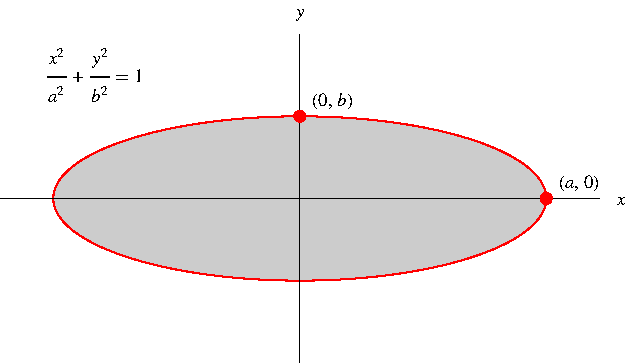
\includegraphics[height=3cm]{trig-substitution/pictures/08-03-ex2a.pdf}%
}%
\only<18->{%
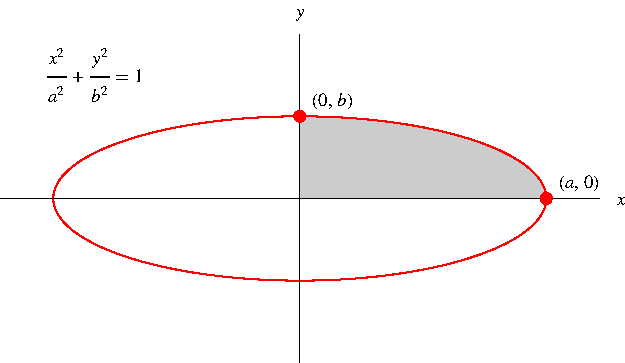
\includegraphics[height=3cm]{trig-substitution/pictures/08-03-ex2b.pdf}%
}%
\end{center}
\end{columns}
\abovedisplayskip=0pt
\belowdisplayskip=0pt
\[
\uncover<2->{%
\alert<12>{%
\sqrt{9 - \alert<7>{x^2}} = 
}%
}%
\uncover<7->{%
\sqrt{9 - \alert<7>{9\sin^2 \theta}} = 
}%
\uncover<8->{%
\sqrt{9 \cos^2 \theta} = 
}%
\uncover<9->{%
3 |\cos  \theta | = 
}%
\uncover<10->{%
\alert<12>{%
3 \cos  \theta  
}%
}%
\]
\abovedisplayskip=0pt
\belowdisplayskip=0pt
\begin{eqnarray*}
\uncover<11->{%
\int \frac{\alert<12>{\sqrt{9-x^2}}}{\alert<14>{x^2}}\alert<13>{\diff x}%
}%
& \uncover<11->{ = } & %
\uncover<11->{%
\int\frac{\alert<12>{3\cos \theta}}{\alert<14>{9\sin^2 \theta}}\alert<13>{3\cos \theta \diff \theta}
}%
\uncover<15->{%
 = \int \cot^2 \theta \diff \theta
}\\%
& \uncover<16->{ = } & %
\uncover<16->{%
 \int (\csc^2 \theta  - 1)\diff \theta
}  \uncover<17->{ = }  \uncover<17->{%
 -\alert<20-21>{\cot \theta} - \theta + C
}\\%
& \uncover<21->{ = } & %
\uncover<21->{%
 -\alert<21>{\frac{\sqrt{9-x^2}}{x}} - \sin^{-1}\left( \frac{x}{3}\right) + C
}%
\end{eqnarray*}
\end{example}
\end{frame}
% end module trig-substitutions-ex2

%%begin module area-under-hyperbola-ex1

\begin{frame}
Recall Euler substitution: $x=\frac12\left(\frac{1}{t}- t \right)$, $\alert<2>{\sqrt{x^2+1}=\frac{1}2\left(\frac 1 t +t\right)}$, $\alert<12,13,14>{ t=\sqrt{x^2+1}-x} $, $\alert<3>{ \diff x=-\frac12 \left(\frac1{t^2} +1\right)\diff t}$.
\begin{example}
$
\begin{array}{rcl}
\displaystyle \int \alert<2>{ \sqrt{x^2+1}} \alert<3>{\diff x} \vphantom{ \frac{1}{8}\left(\frac{1}{ (\sqrt{ x^2 +1} -x)^2} - (\sqrt{x^2+1}- x)^2 \right) } &=&
\displaystyle
\only<1-16>{
\uncover<2->{ \alert<3>{-} \int  \alert<2>{\alert<4>{\frac12} \left(\alert<5,6>{\frac1t} +\alert<7,8>{t}\right)} \alert<3>{\alert<4>{ \frac{1}{2}} \left(\alert<5,7>{ \frac 1 {t^2}} +\alert<6,8>{1} \right)\diff t}} \\
\uncover<4->{ &=&\displaystyle -\alert<4>{ \frac 1 4} \alert<9,10,11>{ \int} \left(\alert<5>{ \alert<9>{ \frac{ 1 }{ t^3}}} + \alert<6,7,10>{2\frac{1}t} + \alert<8,11>{t} \right) \alert<9,10,11>{ \diff t} } \\
\uncover<9->{&=&\displaystyle \alert<15>{-\frac{1}4} \left( \alert<9>{ \alert<15>{ -}\frac{ \alert<12>{ t^{-2}}}{\alert<15>{2}}} +\alert<10>{ \alert<15>{2} \ln\alert<14>{ |t|} }+ \alert<11>{\frac{\alert<13>{ t^2}}{\alert<15>{2}}} \right)+C}\\
\uncover<12->{&=&}
}
\uncover<12->{\displaystyle \only<1-24>{  \alert<16,17,18,24>{ \alert<15>{\frac{1}{8}} \left(\frac{1}{\alert<12>{ (\sqrt{ x^2 +1} -x)^2}} - \alert<13>{\left(\sqrt{x^2+1}- x\right)^2} \right) } }}\only<25->{
\alert<25>{ \frac{1}{2}x\sqrt{x^2+1}}
} {~~~~~~~~~~~~~~~~~~~~~~~~~~~~~~~~~~~~~~~~~~~~~~~~~~~~~~}  \\
\uncover<12->{ && \displaystyle \alert<16,17>{ \only<1-30>{\alert<15>{ -}} \only<31->{\alert<31>{+} } \alert<15>{ \frac12}  \alert<26,30>{\ln \left( \alert<14>{ \sqrt{x^2+1} \only<1-30>{-}\only<31->{\alert<31>{+} } x} \right)} +C}}
\end{array}
$

\noindent \only<17-25>{The answer is good. However, let's simplify.

\noindent
\uncover<18->{
$
\begin{array}{l}
\phantom{=}
\displaystyle \alert<18>{ \frac{1}{(\sqrt{x^2+1}-x)^2}- \left( \sqrt{ x^2+1 }-x\right)^2} \\
\uncover<19->{= \displaystyle \frac{ \alert<19>{(\sqrt{x^2+1} +x )^2} }{ ( \sqrt{x^2 +1} -x )^2  	\alert<19>{(\sqrt{x^2+1}+x)^2} } - \left(\sqrt{x^2+1}-x\right)^2} \\
\uncover<20->{ =\displaystyle \frac{(\sqrt{x^2+1}+x)^2}{ \alert<20>{ \alert<21,22>{((\sqrt{x^2 +1 } )^2 -x^2 )^2 } \uncover<21,22>{\alert<21,22>{=1}} } } - \left( \sqrt{x^2 +1 } -x \right)^2} \\
\displaystyle \uncover<22->{=\left(\sqrt{x^2+1}+x\right)^2-\left( \sqrt{ x^2 + 1 } -x\right)^2} \uncover<23->{ = \alert<24,25>{ 4x\sqrt{x^2+1}}}
\end{array}
$
} %uncover<18->
} %only<17-25>

\only<26->{
The last expression can be transformed to:
\[
\begin{array}{rcl}
\displaystyle
\alert<26>{\ln} \left(\frac{\alert<26,28>{\left(\sqrt{x^2+1}-x\right)} \uncover<27->{ \alert<27,28>{\left( \sqrt{x^2+1}+ x \right)} }}{ \uncover<27->{ \alert<27>{ \sqrt{x^2 +1} +x}}} \right)
&=& \displaystyle \uncover<28->{\alert<29>{ \ln \left( \frac{\alert<28>{ 1} }{ \sqrt{x^2+1}+x}\right)} }\\ \uncover<29->{&=&\alert<29,30,31>{ -\ln \left(\sqrt{x^2+1}+x\right)}}
\end{array}
\]
}
\end{example}

\vspace{8cm}
\end{frame}

\begin{frame}
\begin{example}
Find the area locked b-n the hyperbolas $\alert<2,3>{ y=\pm \sqrt{ x^2+1}}$ and $x=\pm 2\sqrt{ 2}$.
\begin{columns}
\column{.5\textwidth}
\psset{xunit=0.7cm, yunit=0.7cm}
\begin{pspicture}(-3.328427, -3)(3.328427,3)
\psframe*[linecolor=white](-3.328427,-3)(3.328427,3)
\tiny
\uncover<31->{
\pscustom*[linecolor=\fcColorAreaUnderGraph]{
\psplot[linecolor=\fcColorGraph, plotpoints = 1000 ] {-2.828427} {2.828427}{1 x 2 exp add 0.5 exp }
\psline[linecolor=\fcColorGraph](2.828427,-3)(2.828427,3)
\psplot[linecolor=\fcColorGraph, plotpoints=1000] { 2.828427 } {-2.828427}{1 x 2 exp add 0.5 exp -1 mul }
\psline[linecolor=\fcColorGraph](-2.828427,-3)(-2.828427,3)
}
}
\uncover<1-26,28->{
\psaxes[arrows=<->,ticks=none, labels=none](0,0)(-3,-3)(3,3)
}
\psline[linecolor=red!1](3.301,2)(3.302,2)
\psline[linecolor=red!1](-3.301,2)(-3.302,2)

%Function formula: - (x^{2}+1)^{1/2}
\psplot[linecolor=\fcColorGraph, plotpoints=1000]{-2.828427}{2.828427}{1 x 2 exp add 0.5 exp -1 mul }
\uncover<3-4>{\rput[tl](-2.2, -2.4){ \alert<3>{ $y= - \sqrt{ x^2 +1 }$}}}

%Function formula: (x^{2}+1)^{1/2}
\psplot[linecolor=\fcColorGraph, plotpoints=1000]{-2.828427}{ 2.828427 }{1 x 2 exp add 0.5 exp }
\uncover<2-4>{\rput[bl](-2.1, 2.4){\alert<2>{ $y=\sqrt{ x^2 +1} $}}}

\uncover<29->{
\psline[linecolor=\fcColorGraph](-2.828427,3)(-2.828427,-3)
}
\uncover<30->{
\psline[linecolor=\fcColorGraph](2.828427,3)(2.828427,-3)
}
\uncover<25-27>{
\psline{<->}(-2.9,2.9)(2.9,-2.9)
\rput[t](-2.1, 1.7){$\begin{array}{l} \alert<25>{v=0} \\\uncover<1-26>{\alert<25>{y+x=0}} \end{array}$}
}
\uncover<15-27>{
\psline{<->}(-2.9,-2.9)(2.9,2.9)
\rput[b](-2.1, -1.9){$\begin{array}{l} \uncover<1-26>{ \alert<15>{ y-x=0 }}\\\uncover<16->{\alert<16>{u=0}} \end{array}$}
}
\uncover<17-26>{
\fcFullDot{1.4}{1.4}
\rput[l]( 1.6, 1.4){$(\frac{y+x}{2},\frac{y+x}{2})$}
}
\uncover<14-26>{
\fcFullDot{0.6}{2.2}
\rput[lb](0.65, 2.2){$(x,y)$}
}
\uncover<26>{
\psline(0.6,2.2)(-0.8,0.8)
\psline(-0.7, 0.9)(-0.6, 0.8)(-0.7, 0.7)
\rput[rb](-0.3, 1.3){\alert<26>{$v$}}
}
\uncover<18-26>{
\psline(0.6,2.2)(1.4, 1.4)
\psline(1.3, 1.5)(1.2,1.4)(1.3, 1.3)
}
\uncover<23-26>{
\rput[tr](0.95, 1.8){\alert<23>{$u$}}
}
\uncover<14-26>{
\fcFullDot{2.2}{0.6}
\rput[lt]( 2.2, 0.65){$(y,x)$}
}
\end{pspicture}

\vbox to 3.0cm {
\uncover<18->{\alert<18>{
\uncover<22->{\alert<22>{Signed}} distance b-n $(x,y)$ and line $u=0$ equals}}
\only<1-23>{
$\uncover<19->{\uncover<22->{\alert<22>{\pm}} \alert<19>{ \sqrt{ \alert<20>{ \left(x-\frac{(x+y)}{2} \right)^2+ \left( y- \frac{(x+y )}{2} \right)^2}}}}
$
$\uncover<20->{=\uncover<22->{\alert<22>{\pm}} \sqrt{ \alert<20>{ \frac{1}{2}(y-x)^2 }}} \uncover<21->{= \alert<21>{ \uncover<1-21>{\pm} \alert<23>{ \frac{\sqrt{2 }}{ 2 } ( y-x)}}} \uncover<23>{ \alert<23>{=}}$
} %only<1-23>
\uncover<23->{ \alert<23,24>{$u $}.}
\only<24->{\uncover<25->{
Similarly compute that \alert<26>{signed distance b-n $(x,y)$ and the \alert<25>{line $v=0$} equals $v$}.
\uncover<27->{$\Rightarrow$ $y^2-x^2=1$ is the \alert<27>{ hyperbola $v=\frac{1/2}{v}$} in the $(u,v)$-plane.}
}}

\vfil
} %vbox

\column {.5\textwidth}
\only<1-27>{
\uncover<4->{We studied $\alert<27>{v=\frac{1/2}{u}}$ is called a hyperbola:}\uncover<3->{ why do we call $y= \sqrt{ x^2 +1}$ hyperbola?} \uncover<5->{Compute:}
\[
\begin{array}{rcl}
\uncover<5->{\sqrt{x^2+1} &=& y}\\
\uncover<6->{ x^2+1 &=& y^2}\\
\uncover<7->{y^2-x^2&=&1}\\
\uncover<8->{\uncover<9>{\alert<9>{\frac{1}{2}}} \uncover<10->{\alert<10,11>{\frac{\sqrt{2}}{2}}} \alert<11>{(y-x)} \uncover<10->{\alert<10,12>{\frac{\sqrt{2}}{2}}} \alert<12>{(y+x)}&=&\uncover<9->{\alert<9>{\frac{1}{2}}} \uncover<8>{1}}\\
\uncover<11->{\alert<11>{u}\alert<12>{v}&=& \frac{1}{2}}\\
\uncover<13->{\alert<27>{v}&\alert<27>{=}& \alert<27>{\frac{1/2}{u}},}
\end{array}
\]
\uncover<11->{where $\begin{array}{|l}
\alert<11,16,23>{u=\frac{\sqrt{2}}{2} \left(y-x\right)}\\
\alert<12,25>{v=\frac{\sqrt{2}}{2}\left(y+x\right)}
\end{array}$. } \uncover<14->{Consider an arbitrary point $(x,y)$.}
} %only<1-27>
\only<28->{
The area in question is:
$
\begin{array}{l}
\displaystyle\phantom{=} \int \limits^{{{\uncover<28,29>{\alert<29>{ \textbf{?}}}\uncover<30->{\alert<30>{ 2\sqrt{2}}}}}}_{\uncover<28>{\alert<28>{\textbf{?}}}\uncover<29->{ -2\sqrt{2}}} 2\sqrt{x^2+1}\diff x \\
\displaystyle \uncover<32->{= \uncover<33->{\alert<33>{2}} \left[x\sqrt{x^2+1} \vphantom{\ln \left(\sqrt{x^2+1}+x\right) }\right.}\\
\displaystyle \uncover<32->{\left. \ln \left(\sqrt{x^2+1}+x\right)\right]^{2\sqrt{2}}_{\only<33->{\alert<33>{0}} \uncover<1-32>{-2\sqrt{2}}}}\\
\uncover<34->{=2\left(2\sqrt{2} \sqrt{(2\sqrt{2})^2+1}\right.} \\
\uncover<34->{\left.+ \ln \left(\sqrt{(2\sqrt{2})^2+1}+2\sqrt{2} \right) \right)}\\
\uncover<35->{=12\sqrt{2} +2\ln \left(3+2\sqrt{2}\right )}\\
\uncover<36->{\approx 20.496}
\end{array}
$
}
\end{columns}

\end{example}

\end{frame}

%end module area-under-hyperbola-ex1

%%begin module trig-substitutions-euler-substitutions-table

\begin{frame}
\begin{itemize}
\item Let $R$ be a rational function in two variables.
\item<2-> So far, with linear transformations we converted all integrals of the form $\displaystyle\int R(x, \sqrt{ax^2+bx+c})\diff x$ to one of the three forms:

\alert<4,9>{$\int R(x, \sqrt{x^2+1})\diff x$}, \alert<5,10>{$\int R(x, \sqrt{-x^2+1})\diff x$} , \alert<6,11>{$\int R(x, \sqrt{x^2-1}) \diff x$}.
\item<3-> Each of the above integrals can be transformed to a rational trigonometric integral using 3 pairs of substitutions:

\alert<4,9>{$x=\tan\theta $, $x=\cot \theta$;}  
\alert<5,10>{$x=\sin\theta $, $x=\cos \theta$;}
\alert<6,11>{$x=\csc\theta $, $x=\sec \theta$.}
\item<7-> We studied that trigonometric integrals are converted to rational function integrals via $\theta=2\arctan t$.
\item<8-> The resulting 3 pairs of substitutions are called Euler substitutions:
\alert<9,13>{$x=\tan (2\arctan t) $, $x=\cot (2\arctan t)$;}  
\alert<10,13>{$x=\sin(2\arctan t) $, $x=\cos (2\arctan t)$;}
\alert<11,13>{$x=\csc(2\arctan t) $, $x=\sec (2\arctan t)$.}
\item<12-> The Euler substitutions directly transform the integral to a rational function integral.
\item<13-> We will demonstrate that the Euler substitutions are \alert<13>{rational}.
\end{itemize}

\end{frame}

\begin{frame}
\frametitle{Trigonometric substitution and Euler substitution}
{\tabcolsep=0.11cm
\noindent\begin{tabular}{|l|l|l|r|}
\hline
Expression & Substitution& Variable range & Relevant identity\\\hline
\multirow{2}{*}{$\sqrt{x^2+1}$} & $x = \tan \theta$ &  $ \theta\in \left(-\frac{\pi}{2} , \frac{\pi}{2}\right)$ & $1 + \tan^2 \theta = \sec^2 \theta$\\
&$x=\cot \theta$ &$ \theta\in (0, \pi) $ & $1+\cot^2\theta =\csc^2\theta $ \\ \hline 
\multirow{2}{*}{ $\sqrt{-x^2+1 }$} & $x = \sin \theta$ &  $ \theta\in \left[ -\frac{\pi}{2} ,\frac{\pi}{2}\right]$ & $1 - \sin^2 \theta = \cos^2 \theta$\\
& $x = \cos \theta$ & $\theta\in (0,\pi)$& $1-\cos^2\theta=\cos^2\theta$ \\\hline 
\multirow{2}{*}{$\sqrt{x^2-1}$} & $x = \sec \theta$ & 
$\theta\in \left[0, \frac{\pi}{2}\right)\cup \left[\pi, \frac{ 3 \pi}{2}\right)$
& $\sec^2\theta - 1 = \tan^2\theta$\\
&$x=\csc \theta$ &$\theta\in \left[0, \frac{\pi}{2} \right) \cup \left[ \pi, \frac{3\pi}{2}\right)$ &  $\csc^2\theta=\cot^2\theta $\\
\hline
\multicolumn{4}{c}{Euler substitution by applying in addition $\theta=2\arctan t$}\\
\hline
\multirow{2}{*}{$\sqrt{x^2+1}$} & $ x =\frac{2t}{1-t^2}$ & $-1< t< 1$ & (?) \\
&$ x=\frac{1}{2} \left(\frac{1}{t}-t\right)$ & $0<t $ &  (?)\\ \hline 
\multirow{2}{*}{ $\sqrt{-x^2+1 }$} & $x=\frac{2t}{1+t^2} $ & $-1\leq t\leq 1 $ & (?)\\
& $x =\frac{1-t^2}{1+t^2} $ & $0<t$&  (?)\\\hline 
\multirow{2}{*}{ $\sqrt{x^2-1}$} & $x=\frac{1}{2}\left(\frac{ 1}{t}+t\right)$ & $t\in (-\infty, -1)\cup [0,1)$&(?)\\
& $x =\frac{1+t^2}{1-t^2} $ & $t \in (-\infty,-1)\cup [0,1)$ & (?)\\\hline
\end{tabular}
}
\end{frame}
%end module trig-substitutions-euler-substitutions-table

%%begin module trig-substitution-case-1-cot
\begin{frame}
\frametitle{Trigonometric substitution $x=\cot \theta$  for $\sqrt{ x^2+1}$}
The trigonometric substitution $ \alert<2,13>{x=\cot \theta}$, $\theta\in \left(0 , \pi\right) $ for $\sqrt{x^2+1}$:
\[
\begin{array}{rclll}
\displaystyle  \alert<8,9,12>{\sqrt{\alert<2>{x}^2+1}}
\vphantom{\frac{1}{\sin \theta}}
\only<1-8>{
&=&\displaystyle \uncover<2->{ \sqrt{\alert<3>{\alert<2>{\cot}^2 \alert<2>{ \theta} } +1} }\\
\uncover<3->{&=&\displaystyle \sqrt{\alert<4>{\alert<3>{\frac{\cos^2 \theta }{ \sin^2 \theta}} + 1} }} \\
\uncover<4->{&=&\displaystyle \sqrt{ \alert<4>{\frac{\alert<5>{ \cos^2 \theta+ \sin^2\theta}}{ \sin^2 \theta}}}} \\
\uncover<5->{&=& \displaystyle  \sqrt{\frac{\alert<5>{ 1} }{ \sin^2 \theta}}=\frac{1}{\alert<6>{\sqrt{\sin^2\theta}}} } \uncover<6->{ && 
\begin{array}{|l}\displaystyle \text{when }\theta\in \left(0 , \pi\right) \text{ we have }\\ ~ \sin \theta \geq 0\text{ and so } \\ \alert<6>{ \sqrt{\sin^2 \theta}=\sin\theta}  \end{array} }
\\
} %only<1-8>
\uncover<6->{&\alert<8,9,12>{ =}& \displaystyle  \alert<8,9,12>{\frac{1}{\alert<6>{ \sin \theta} }}} \uncover<7->{\alert<8,9,12>{= \csc \theta \quad . }} && {~~~~~~~~~~~~~~~~~~} {~~~~~~~~~~~~~~~~~~~~} {~~~~~~~~~~~~~~~~~~~} %white space flushes formulas to the left
\end{array}
\]
\uncover<10->{
The differential $\diff x$ can be expressed via $\diff \theta$ from $x=\cot \theta$. \uncover<11->{
To summarize:
\begin{definition}The trigonometric substitution $\alert<13>{ x=\cot \theta }$, $\theta\in (0,\pi)$ for $\sqrt{x^2+1} $ is given by:
\[
\begin{array}{rcl}
x &=&\displaystyle \cot \theta \\
\alert<12>{\sqrt{x^2+1}}&\alert<12>{=}&\displaystyle \alert<12>{\frac{1}{\sin \theta}=\csc \theta}\\
\alert<14,15>{\diff x} &\alert<14,15>{=}&\displaystyle \uncover<15->{\alert<15>{ -\frac{\diff \theta}{\sin^2\theta} = - \csc^2 \theta} } \uncover<1-14>{\alert<14>{\textbf{?}}} \alert<14,15>{\diff \theta}\\
\alert<13>{\theta}& \alert<13>{=}& \alert<13>{\Arccot x}\quad .
\end{array}
\]
\end{definition}
}
}

\vspace{10cm}
\end{frame}
%end module trig-substitution-case-1-cot
%%begin module Euler-substitution-case-1-cot
\begin{frame}
\frametitle{Euler subst. for $\sqrt{x^2+1}$ corresponding to $x=\cot \theta$ }
\begin{itemize}
\item $\alert<4>{ x =\cot \theta}$ transforms $\diff x, x,\sqrt{x^2+1}$ to trig form.
\item $\alert<5>{\theta=2\Arctan t}$, \uncover<3->{ $t>0$} transforms $\diff \theta, \cos\theta,\sin \theta$ to rational form.
\end{itemize}
\uncover<2->{\alert<2>{What if we compose the above?}} \uncover<3->{\alert<3>{We get the Euler substitution:}}
\only<1-34>{ %
\[
\begin{array}{rclll}
\uncover<3->{\alert<4,16,26,33,34>{x}} 
\vphantom{\frac{1}{2}\left(\frac{1}t - t\right)}
&\uncover<3->{\alert<4,16,26,33,34>{=}} &\displaystyle 
\vphantom{\frac{1}{2}\left(\frac{1}t -t\right)} %phantom
\only<3-13>{
\displaystyle \uncover<4->{\alert<4>{ \cot\alert<5>{\theta}}} \\
\uncover<5->{&=& \displaystyle \alert<8>{\cot \left(\alert<5>{2\arctan t}\right)}} \uncover<6->{&&| \displaystyle  \text{Recall: } \alert<8>{\cot (2z)} =\frac{ \cos (2z)}{\sin (2z)} \uncover<7->{\alert<8>{=\frac{1-\tan^2z}{2\tan z }}}} \\
\uncover<8->{ &=&\displaystyle \alert<8>{ \frac{1-{\alert<9>{\tan}}^2 \alert<9>{(\arctan t)}}{2 \alert<9>{\tan (\arctan t)}}}} \\
\uncover<9->{&=&\displaystyle \alert<16>{\frac{\alert<11>{1}-\alert<12>{{\alert<9>{t}}^2}}{\alert<10>{2} \alert<9,11,12>{t}}}}\\
\uncover<10->{&=&}
} %only <3-13>
\uncover<10->{\displaystyle \alert<13,14,16,26,33,34>{ \alert<10>{ \frac{1}{2}}\left(\alert<11>{\frac{1}t} - \alert<12>{t} \right)}\quad . &&
{~~~~~~~~~~~~~~~~~~~~~~~~~~~~~~~~~~~~~~~~~~~~~~~~~~~~~~~~~~~~~~~~~~~~~~~~~~~~~} %whitespace flushes formulas left
}
\end{array}
\]
\uncover<15->{
We can furthermore compute 
\[
\begin{array}{rclll}
\displaystyle 
\alert<32,34>{\sqrt{x^2+1}}& \alert<32,34>{=}& 
\only<1-23>{
\displaystyle  \uncover<16->{ \sqrt{ \alert<16>{\alert<17>{\frac{1}{4}} \left(\frac{1}t -t \right)^2} +\alert<17>{1}}}\\
\uncover<17->{ &=&\displaystyle \alert<17>{\frac{1}{2}} \alert<22>{ \sqrt{\alert<19>{\left( \frac{1}{t} \only<1-19>{-}\only<20->{\alert<20>{+}} t \right)^2\uncover<1-19>{+\alert<17>{4}}}}}} & &
\only<18,19>{
\begin{array}{|l} 
\alert<19>{\left(\frac{1}{t}- t\right)^2+4=\left(\frac{1}{t}\alert<18>{+}t\right)^2 }
\end{array}
} 
\uncover<21->{ 
\begin{array}{|l}
\alert<22>{\sqrt{\left(\frac{1}{t}+t\right)^2} = \frac{1}{t} +t}\\ \text{ because }t>0
\end{array}
} %uncover<21->
\\
&\uncover<22->{=}&
} %only<1-23>
\uncover<22->{ \displaystyle \alert<23,24,32,34>{ \frac{1}{2}\left(\alert<22>{\frac{1}{t}+t}\right)} 
\vphantom{\sqrt{ \frac{1}{4} \left(\frac{1}t -t \right)^2 }}
\quad . &&} {~~~~~~~~~~~~~~~~~~~~~~~~~~~~~~~~~~~~~~~~~~~~~~~~~~~~~~~~~~~~~~~~~} %whitespace flushes formulas left
\end{array}
\]
}
\uncover<25->{
Finally compute 
\[
\begin{array}{rcl}
\alert<34>{\diff \alert<26>{x}}&=&\displaystyle  \uncover<26->{\alert<27,28>{\diff \left( \alert<26>{\frac{1}{2} \left(\frac{1}t -t\right)} \right)}}\uncover<27->{\alert<27,28,34>{=}} \uncover<28->{\alert<28,34>{-\frac12 \left( \frac{1}{t^2} +1\right) \diff t}}\\
\displaystyle \uncover<29->{  \alert<30,34>{t}}&\uncover<29->{=} &\displaystyle  \uncover<29->{\alert<32>{ \alert<30,31>{\frac{1}{2}} \left(\alert<31>{\frac{1 }{ t}} +\alert<30>{t}\right)} \alert<30,31>{-} \alert<33>{\alert<30,31>{ \frac{1}{2}} \left(\alert<31>{ \frac{1}{t}} \alert<30>{- t}\right)}\uncover<32->{\alert<34>{ = \alert<32>{\sqrt{ x^2 +1}} -\alert<33>{x}}}\quad .} 
\end{array}
\]
}
} %only <1-34>
\uncover<35->{
\begin{definition}The Euler substitution for $\sqrt{x^2+1}$ corresponding to $x=\cot \theta$ is given by:
\[
\begin{array}{rcl}
\alert<35>{x} &\alert<35>{=}&\displaystyle \alert<35>{\frac12\left(\frac{1}{t}- t\right) }, \quad \quad t>0\\
\displaystyle \alert<35>{ \sqrt{x^2+1}} & \alert<35>{=}& \displaystyle \alert<35>{\frac12 \left(\frac1t +t\right)} \\ 
\displaystyle \alert<35>{ \diff x}& \alert<35>{=}&\displaystyle \alert<35>{-\frac12\left(\frac{1}{t^2}+1\right) \diff t}\\
\alert<35>{t} &\alert<35>{=}&\alert<35>{\sqrt{x^2+1}-x}\quad .
\end{array}
\]
\end{definition}

\vspace{5cm}
}
\end{frame}

%end module Euler-substitution-case-1-cot
%\subsubsection{Trigonometric substitution $x=\cos \theta$, $\theta\in\left[0, \pi\right] $}
The trigonometric substitution $x=\cos \theta$ is given by 
\[
\begin{array}{rcll|l}
\displaystyle \sqrt{-x^2+1}&=&\displaystyle \sqrt{1-\cos^2\theta}\\
&=&\displaystyle \sqrt{\sin^2\theta} &&\begin{array}{l} \text{when }\theta\in\left[-\frac{\pi}{2}, \frac{\pi}{2} \right] \text{we have}\\
\sin \theta\geq 0 \text{ and so } \sqrt{\sin^2\theta}=\sin \theta
\end{array} \\
&=&\displaystyle \sin \theta\quad .
\end{array}
\]
The differential $\diff x$ can be expressed via $\diff \theta$ from $x=\cos \theta$. The substitution $x=\cos \theta $ can be now summarized as:
\begin{equation*}
\begin{array}{rcl}
x&=&\cos \theta\\
\sqrt{-x^2+1}&=&\cos \theta\\
\diff x&=& -\sin \theta \diff \theta\\
\theta&=&\arccos x \quad .
\end{array}
\end{equation*}
%\begin{frame}
\frametitle{Euler subst. for $\sqrt{-x^2+1}$ corresponding to $x=\cos \theta$ }
\begin{itemize}
\item $\alert<4>{ x =\cos \theta}$ transforms $\diff x, x,\sqrt{-x^2+1}$ to trig form.
\item $\alert<5>{\theta=2\Arctan t}$, \uncover<3->{ $t>0$} transforms $\diff \theta, \cos\theta,\sin \theta$ to rational form.
\end{itemize}
\uncover<2->{\alert<2>{What if we compose the above?}} \uncover<3->{\alert<3>{We get the Euler substitution:}}
\only<1-37>{ %
\[
\begin{array}{rclll}
\uncover<3->{\alert<4,13,22,33,37>{x}}&\uncover<3->{\alert<4,13,22,33,37>{=}}&\displaystyle \vphantom{\frac{1- t^2}{ 1+ t^2} } 
\only<1-10>{
\displaystyle \uncover<4->{\alert<4>{ \cos \alert<5>{\theta}} } \\
\uncover<5->{ &=&\displaystyle \alert<8>{ \cos (\alert<5>{2\arctan t})}} \uncover<6->{&&\begin{array}{|l}
\displaystyle \displaystyle \alert<6,7,8>{\cos (2z) =}\uncover<7->{\alert<7,8>{ \frac{ 1-\tan^2 z }{1+ \tan^2 z}}}
\end{array}}
\\
\uncover<8->{ &=&\displaystyle \alert<8>{ \frac{1- {\alert<9>{\tan}}^2 ( \alert<9>{\Arctan t})}{1+{\alert<9>{\tan}}^2(\alert<9>{\Arctan t})} } } \\
\uncover<9->{&=&}
} %only<1-10>
\uncover<9->{\displaystyle \alert<10,11,13,22,33,37>{ \frac{\alert<22>{ 1- { \alert<9>{t}}^2}}{\alert<23>{ 1+ { \alert<9>{t}}^2}} }  &&{~~~~~~~~~~~~~~~~~~~~~~~~~~~~~~~~~~~~~~~~~~~~~~~~~~~~~~~~~~~~~~~~~~~~~~~~~~~~~~~~~} %whitespace flushes formulas left
} 
\uncover<12->{ \\\hline}
\uncover<12->{\alert<37>{ \sqrt{- {\alert<13>{x}}^2+1 }}}&\uncover<12->{\alert<37>{=}} &\displaystyle 
\only<1-20>{
\uncover<13->{ \sqrt{\alert<14>{1} - \left(\alert<13>{ \frac{1-t^2}{ 1+ t^2 }} \right)^2}}\\
\uncover<14->{&=&\displaystyle \sqrt{\frac{ \alert<15>{ \alert<14,17>{ (1+ t^2)^2} -(1-t^2)^2} }{ \alert<14>{(1+t^2)^2}} }}&&
\uncover<15->{\begin{array}{|l}
\alert<15,16>{(1+t^2)^2-(1-t^2)^2=}\only<15>{\alert<15>{\textbf{?}}} \uncover<16->{\alert<16>{4t^2}}}
\end{array} 
\\
\uncover<17->{&=&\displaystyle  \sqrt{\frac{ \alert<17>{4t^2} }{ (1+t^2)^2}}} \uncover<18->{&& 
\begin{array}{|l}
\displaystyle \alert<18>{ \alert<19>{\sqrt{4t^2}=2t} \text{ because } t>0} }
\end{array}
\\
\uncover<19->{&=&}
} %only<1-20>
\uncover<19->{ \displaystyle \alert<20,21,37>{ \frac{{2t} }{1+t^2}} \vphantom{ \sqrt{1 - \left( \frac{1-t^2}{ 1+ t^2 } \right)^2}} }\uncover<22->{\\\hline }
\only<1-30>{
\uncover<22->{ \displaystyle \alert<23>{ (\alert<25>{1}+ \alert<24>{t^2})} \alert<22,24,25>{ x} &=&\displaystyle  \alert<22>{\alert<25>{1} -\alert<24>{t^2}}}\\
\uncover<24->{ \displaystyle \alert<24>{ t^2(\alert<26>{x+1})}&=&\displaystyle \alert<25>{ 1-x}}\\
\uncover<26->{ \displaystyle t^2&=&\displaystyle \frac{1-x}{\alert<26>{1+x}}}\\
}
\uncover<27->{ \displaystyle \alert<30,31,37>{t}} &\alert<30,31,37>{\uncover<27->{=}}&\displaystyle \only<27-30>{\uncover<27->{ \frac{ \alert<29>{ \sqrt{1 -x }}}{\sqrt{ 1+x}}} \uncover<28->{ \frac{ \alert<29>{  \sqrt{1+x}} }{\sqrt{1+x}} }}\only<29-30>{=} \uncover<29->{ \alert<30,31,37>{ \frac{ \alert<29>{ \sqrt{-x^2+1} }}{x+1}}} && 
\uncover<27-30>{
\begin{array}{l}\text{here we use } t>0
\end{array}
} 
\uncover<31->{ \\\hline}
\uncover<32->{\alert<37>{ \diff \alert<33>{x}}} &\uncover<33->{=} & \displaystyle \vphantom{\diff \left( \frac{ 1- t^2}{ 1+ t^2}\right)} \only<33->{\diff \left( \alert<33>{\frac{ 1- t^2}{ 1+ t^2}}\right)} 
\only<34->{=\diff\left(\frac{2-\alert<35>{ (1+t^2)} }{ \alert<35>{ 1 + t^2}} \right)}\\
&\uncover<35->{=}&\only<35->{\displaystyle \diff\left(\frac{2}{1+ t^2} \alert<35>{-1} \right)}
\only<36->{\alert<37>{=-\frac{4t}{(1+t^2)^2}\diff t}}
\end{array}
\]
} %only<1-37>
\uncover<38->{
\begin{definition}
The Euler substitution for $\sqrt{-x^2+1}$ corresponding to $x=\cos \theta$ is given by:
\[
\alert<38>{
\begin{array}{rcl}
x&=&\displaystyle \frac{1-t^2}{1+t^2}, \quad \quad t>0\\
\sqrt{-x^2+1}&=&\displaystyle \frac{2t}{1+t^2}  \\
\diff x&=&\displaystyle  -\frac{4 t}{(t^{2}+1)^{2}} \diff t\\
t&=&\displaystyle \frac{\sqrt{-x^2+1}}{x+1} \quad .
\end{array}
}
\]
\end{definition}

\vspace{7cm}
}
\end{frame}

%\begin{frame}
\frametitle{Trigonometric substitution $x=\sec \theta$ for $\sqrt{ x^2-1}$ }
The trigonometric substitution $ \alertNoH{10,12}{x=\sec \theta}$, $\theta \in \left[0, \frac{\pi}{2}\right)\cup \left[\pi, \frac{3\pi}{ 2} \right) $:
\[
\begin{array}{rclll}
\displaystyle \alertNoH{11}{\sqrt{x^2-1}}&\alertNoH{11}{=} & \displaystyle
\only<handout:1|1-8>
{\uncover<2->{ \sqrt{\sec^2\theta-1}}\\
\uncover<3->{&=& \displaystyle \sqrt{\frac{1}{\cos^2\theta}-1}}\\
\uncover<4->{&=&\displaystyle \sqrt{\frac{\sin^2\theta}{\cos^2\theta}}} \\
\uncover<5->{&=&\displaystyle \sqrt{ \tan^2 \theta}} &&\uncover<6->{ \begin{array}{|l} \text{when }\theta\in \theta \in \left[0, \frac{ \pi}{2 }\right)\cup \left[\pi, \frac{3\pi}{2}\right) \text{we have}\\
\tan \theta\geq 0 \text{ and so } \sqrt{\tan^2\theta}=\tan \theta
\end{array}} \\
\uncover<7->{&=&}
}
\uncover<7->{\displaystyle \alertNoH{8,9,11}{\tan \theta} \vphantom{\sqrt{\sec^2\theta-1}}\quad .&&{~~~~~~~~~~~~~~~~~~~~~~~~~~~~~~~~~~~~~~~~~~~~~~~~~~~~~~~~~~~~~~~~~~~~~~~~~~~~~~~~~~~~~~~~~~~~~~~~~~~~~~} }
\end{array}
\]
\uncover<handout:2|10->{
\begin{definition}The trigonometric substitution $\alertNoH{10,12}{ x=\sec \theta }$, $\theta\in (0,\pi)$ for $\sqrt{x^2+1} $ is given by:
\[
\begin{array}{rcl}
\displaystyle \alertNoH{10,13}{ x}&\alertNoH{10,13}{=}& \displaystyle \alertNoH{10,13}{\sec\theta= \frac{1}{\cos \theta} } \quad \quad \theta \in \left[0, \frac{\vphantom{3} \pi}{2}\right)\cup \left[\pi, \frac{ 3 \pi}{ 2} \right)\\
\displaystyle \alertNoH{11}{ \sqrt{x^2-1}}&\alertNoH{11}{ =}& \displaystyle \alertNoH{11}{ \tan \theta}\\
\displaystyle \alertNoH{13,14}{\diff x}& \alertNoH{13,14}{=} & \displaystyle \fcAnswerUncover{10}{14}{ \frac{\sin\theta}{ \cos^2\theta} \diff \theta= \sec\theta\tan\theta }  \alertNoH{14}{ \diff \theta} \\
\displaystyle \alertNoH{12}{\theta}&\alertNoH{12}{=} &\alertNoH{12}{ \Arcsec x} \quad .
\end{array}
\]
\end{definition}
}

\vspace{20cm}
\end{frame}

%\begin{frame}
\frametitle{Euler substitution $x=\sec \theta$, $\theta = 2\arctan t$}
\begin{itemize}
\item $\alert<4>{ x =\sec \theta}$ transforms $\diff x, x,\sqrt{x^2+1}$ to trig form.
\item $\alert<5>{\theta=2\Arctan t}$, \uncover<3->{ $ t\in (-\infty, -1) \cup \left[0, 1 \right) $ } transforms $\diff \theta, \cos\theta,\sin \theta$ to rational form.
\end{itemize}
\uncover<2->{\alert<2>{What if we compose the above?}} \uncover<3->{\alert<3>{We get the Euler substitution:}}
\[
\begin{array}{rclll}
\uncover<3->{\alert<4,15>{x}}&\uncover<3->{\alert<4,15>{=}}& \displaystyle  
\only<1-12>{
\uncover<4->{ \alert<4>{\sec \theta} =\frac{1}{\cos \alert<5>{ \theta} }} \\
\uncover<5->{&=& \displaystyle \alert<8>{ \frac{1} {\cos(\alert<5>{ 2\arctan t} )}} } &&
\uncover<6->{
\begin{array}{|l} \displaystyle \alert<8>{ \alert<6,7>{\cos (2z) =} \uncover<7->{\alert<7>{\frac{ 1- \tan^2 z}{1+ \tan^2 z }}}}
\end{array}
}
\\
\uncover<8->{&=& \displaystyle \alert<8>{  \frac{1+ {\alert<9>{\tan}}^2 (\alert<9>{\Arctan t })}{ 1- {\alert<9>{\tan}}^2 (\alert<9>{\Arctan t}) } }}
\\
\uncover<9->{&=&\displaystyle \frac{1+ {\alert<9>{t}}^2 }{1 - { \alert<9>{ t}}^2}}\uncover<10->{=\frac{2\alert<11>{- (1 - t^2 )} }{\alert<11>{1 - t^2} }}  \\
\uncover<11->{&=&} 
}
\uncover<11->{\displaystyle \alert<12,13,15>{ \alert<11>{-1}+\frac{2}{1-t^2}} }
\uncover<13->{\\\hline }
\uncover<14->{\sqrt{{\alert<15>{x}}^2-1 }}&\uncover<14->{=} &\displaystyle \uncover<15->{\sqrt{ \left(\alert<15>{ \frac{1 +t^2 }{\alert<16>{ 1- t^2 }}} \right)^2 -\alert<16>{1}} }\\
\uncover<16->{&=& \displaystyle \sqrt{\frac{ \alert<19>{(1+t^2)^2 - \alert<16>{ (1-t^2)^2}}}{ \alert<16>{(1-t^2)^2} } }} &&
\uncover<17->{
\begin{array}{|l}
\alert<17,18,19>{(1+t^2)^2-(1-t^2)^2= } \only<17>{ \alert<17>{ \textbf{?}}} \uncover<18->{\alert<18,19>{4t^2}}
\end{array}
}
\\
\uncover<19->{ &=& \displaystyle \alert<20>{\sqrt{\frac{ \alert<19>{ 4t^2} } { (1-t^2)^2}}} }&& 
\uncover<20->{\alert<20>{
\begin{array}{|l} \displaystyle t \text{ and }1-t^2\text{ have same sign}\\ \text{when } t\in (-\infty, -1) \cup \left[0, 1 \right)
\end{array}
}
}
\\
\uncover<20>{&=&}
\uncover<20>{ \displaystyle \alert<20>{ \frac{2t}{1-t^2}} \quad .}
\end{array}
\]
The differential $\diff x$ can be computed from $x=\frac{1+t^2}{1-t^2}$. Finally, we can express $t$ via $x$ with a little algebra:
\[
\begin{array}{rcll|l}
\displaystyle x&=&\displaystyle  \frac{1+t^2}{ 1- t^2} \\
\displaystyle (1- t^2)x&=&\displaystyle  1+t^2\\
\displaystyle (1+ x)t^2&=&\displaystyle  x-1\\
\displaystyle t^2&=&\displaystyle  \frac{x-1}{x+1}\\
\\
\displaystyle t&=&\displaystyle %\doublebrace{ \sqrt{\frac{x-1}{x+1}}}{x>1}{-\sqrt{\frac{x-1}{x+1}}}{x<-1} &&\begin{array}{l} \text{because when } x<-1, \\ \text{ we have } t\in \left( -\infty , -1 \right]\end{array} \\
%\displaystyle t&=&\displaystyle \doublebrace{ \frac{\sqrt{ x^2 -1}}{x+1}}{x>1}{-\frac{\sqrt{x^2-1}}{x+1}}{x<-1}  \quad .
\end{array}
\]
The Euler substitution $x= \sec (2\arctan t)$ can be now summarized as:

\[
\begin{array}{rcl}
x&=&\displaystyle \frac{1+t^2}{1-t^2}\\
\sqrt{x^2-1}&=&\displaystyle \frac{2t}{1-t^2}  \\
\diff x&=&\displaystyle  \frac{4 t}{(1- t^{2})^{2}} \diff t\\
t&=&\displaystyle \pm \frac{ \sqrt{x^2-1}}{x+1} \quad .
\end{array}
\]
As demonstrated in the present section, it is sufficient to memorize the substitution $x=\sec (2\arctan t)$ in order to derive the equalities above. An alternative way to memorize the Euler substitution is through the equality
\[
\begin{array}{rcl}
\sqrt{x^2-1}&=&(x+1)t\quad .
\end{array}
\]
\end{frame}
%% begin module inverse-notation-warning
\begin{frame}
\alert<1->{WARNING:}

Do not mistake the $-1$ in $f^{-1}(x)$ for an exponent.
\[
f^{-1}(x) \ \text{does not mean } \ \frac{1}{f(x)} .
\]

If you want to write $\frac{1}{f(x)}$ using exponents, you can write $(f(x))^{-1}$.
\begin{itemize}
\item<2->  $f^{-1}(x)$ is the compositional inverse of $f$.
\item<3->  $\frac{1}{f(x)}$ is the multiplicative inverse of $f$.
\end{itemize}
\end{frame}
% end module inverse-notation-warning

%% begin module parametric-intro
\begin{frame}
\frametitle{Curves Defined by Parametric Equations}
\begin{columns}[c]
\column{.4\textwidth}

\psset{xunit=1cm, yunit=1cm}
\begin{pspicture}(-1.000000, -5)(1.500000,5) 
\psframe*[linecolor=white](-1.000000,-5)(1.500000,5) 
\tiny 
\psaxesStandard{-2}{-0.5}{2}{3.5}
%Calculator input: plotCurve{}(\cos{}(t^{2}), t \sin{}t+\sin{}t, 0, 3)
\parametricplot[arrows=->, linecolor=\psColorGraph, plotpoints=500] {0}{0.75}{t 2 exp 57.29578 mul cos t 57.29578 mul sin t 57.29578 mul sin t mul add }
\parametricplot[arrows=->, linecolor=\psColorGraph, plotpoints=500] {0.75}{1.5}{t 2 exp 57.29578 mul cos t 57.29578 mul sin t 57.29578 mul sin t mul add }
\parametricplot[arrows=->, linecolor=\psColorGraph, plotpoints=500] {1.5}{2.25}{t 2 exp 57.29578 mul cos t 57.29578 mul sin t 57.29578 mul sin t mul add }
\parametricplot[linecolor=\psColorGraph, plotpoints=500] {2.25}{3}{t 2 exp 57.29578 mul cos t 57.29578 mul sin t 57.29578 mul sin t mul add }

\uncover<1>{\psFullDot{0.987227}{ 0.545186} } 
\uncover<2>{\psFullDot{0.689498}{ 1.488321} }
\uncover<3>{\psFullDot{-0.379452}{ 2.365079}}
\uncover<4>{\psFullDot{-0.892288}{ 2.744270}}
\uncover<5->{\psFullDot{0.866232}{ 2.296575} }
\uncover<6->{
\rput[l](0.89,2.396575){$\begin{array}{l}(x,y)\uncover<7->{= (g(t), f(t))} \\\phantom{(x,y)}\uncover<8->{=(x(t), y(t))}\end{array}$}
}
\end{pspicture} 
%\ \only<handout:0| -1>{%
%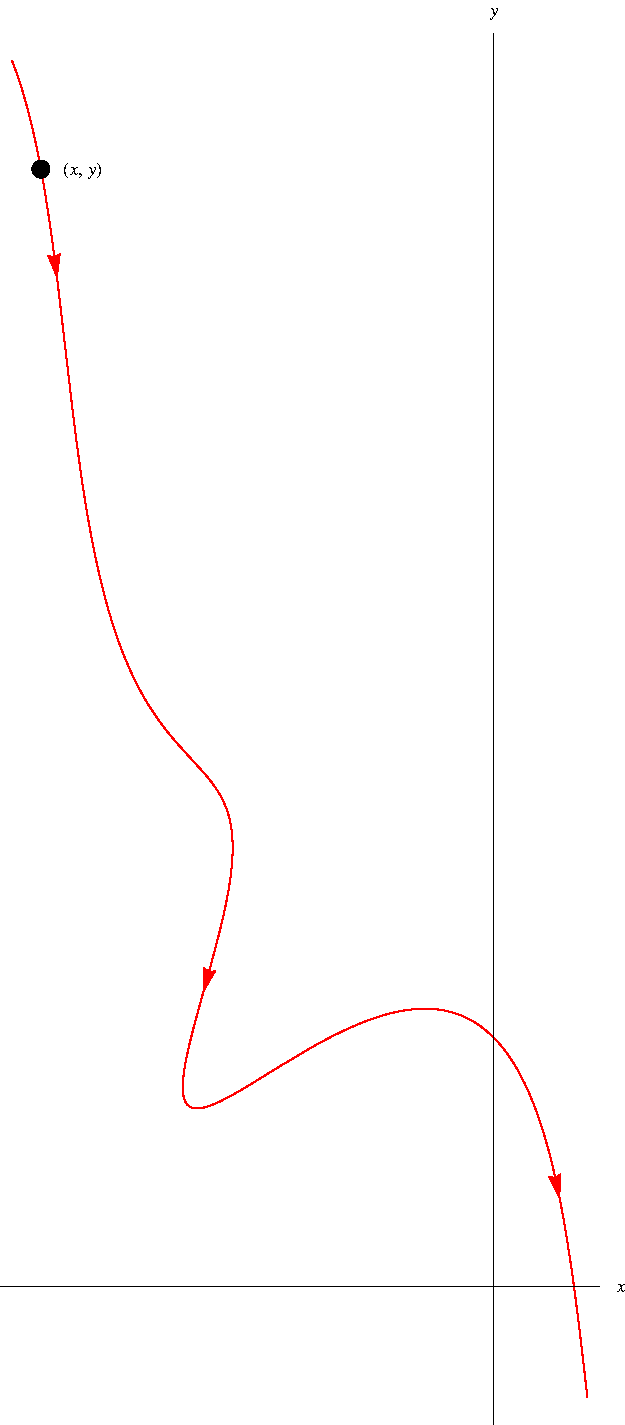
\includegraphics[height=7cm]{parametric-curves/pictures/11-01-parametrica.pdf}%
%}%
%\only<handout:0| 2>{%
%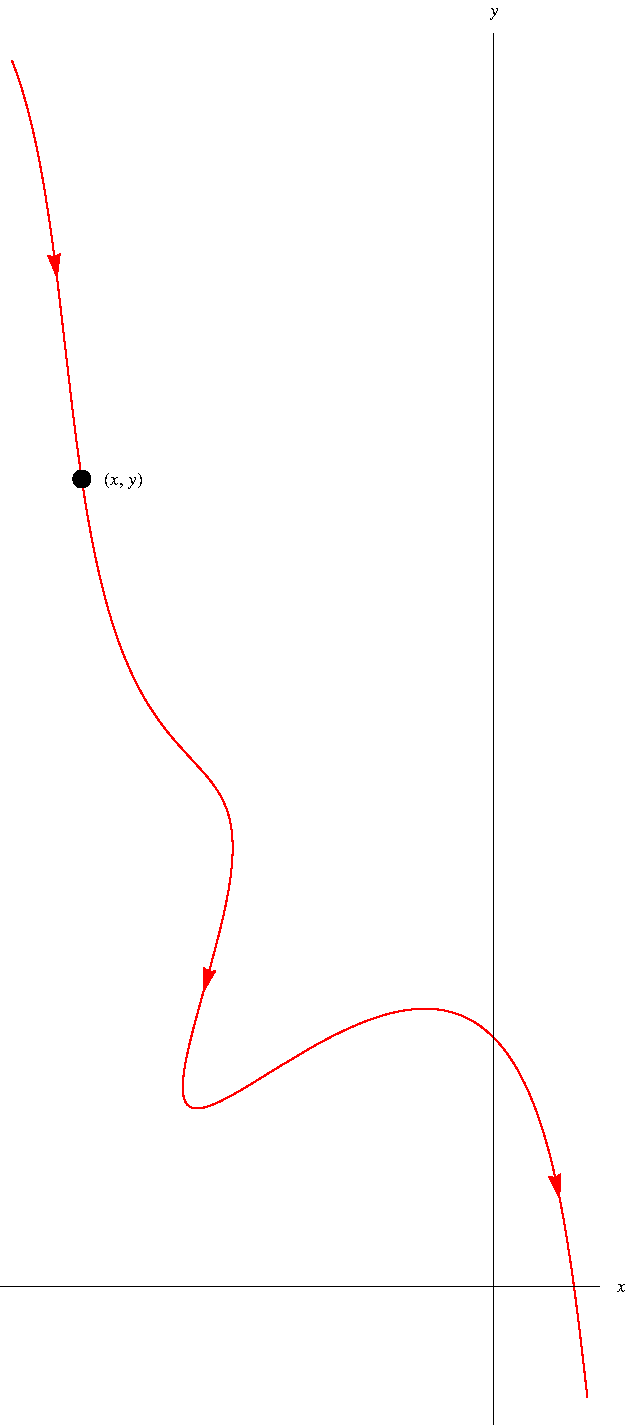
\includegraphics[height=7cm]{parametric-curves/pictures/11-01-parametricb.pdf}%
%}%
%\only<handout:0| 3>{%
%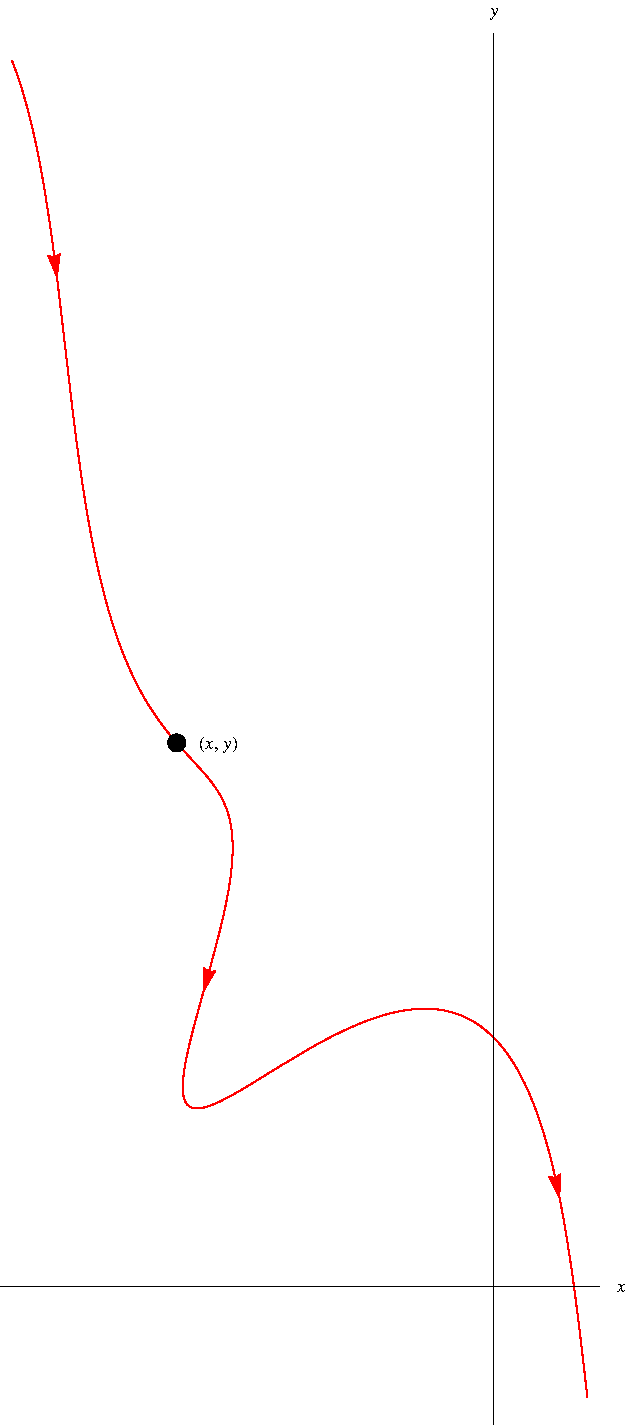
\includegraphics[height=7cm]{parametric-curves/pictures/11-01-parametricc.pdf}%
%}%
%\only<handout:0| 4>{%
%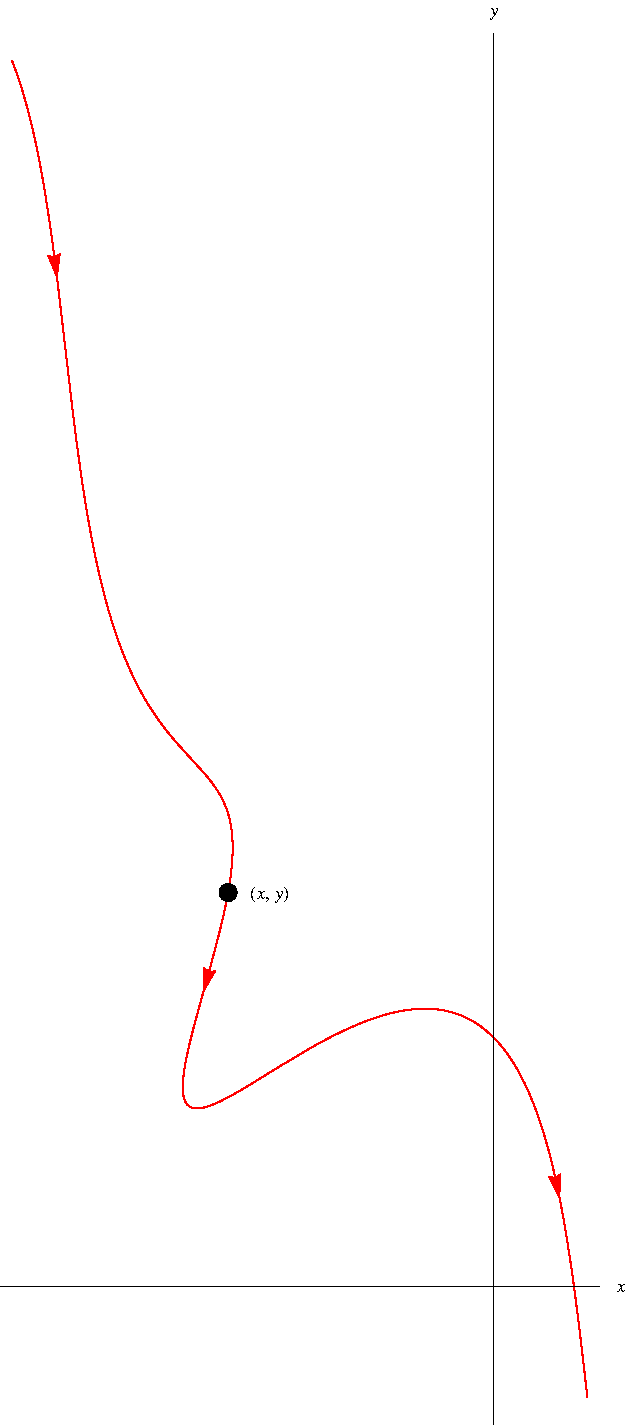
\includegraphics[height=7cm]{parametric-curves/pictures/11-01-parametricd.pdf}%
%}%
%\only<handout:0| 5-7>{%
%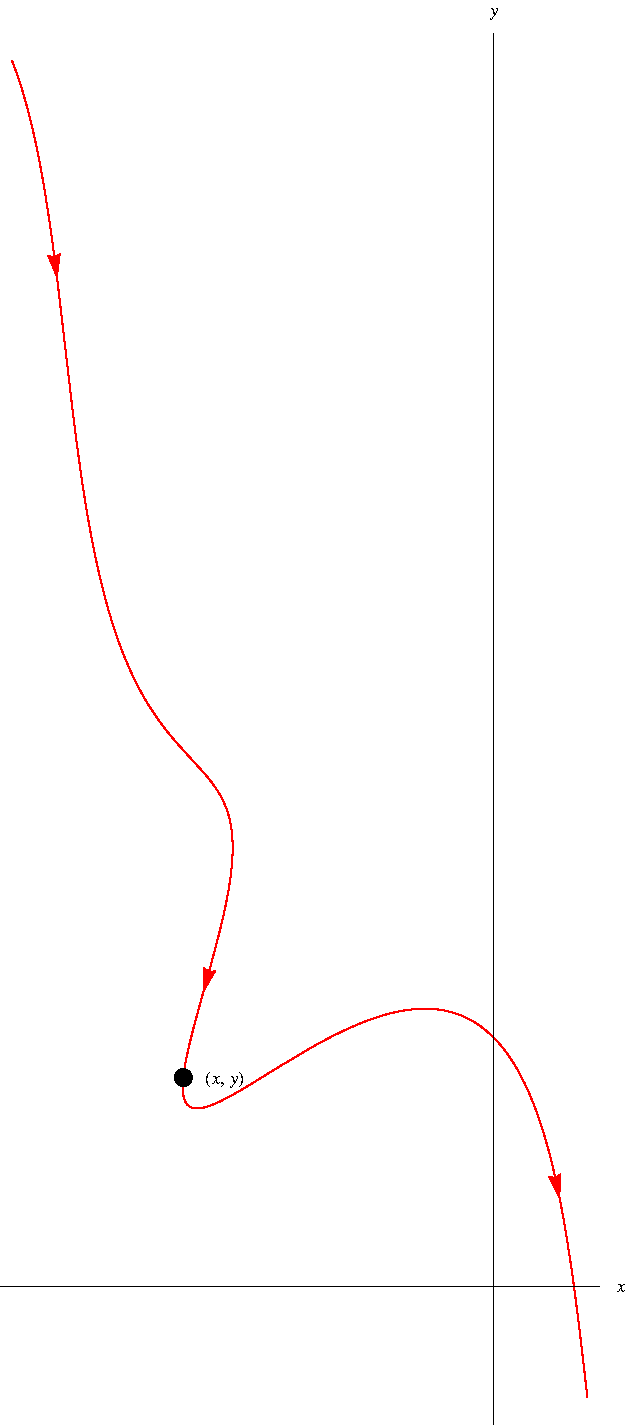
\includegraphics[height=7cm]{parametric-curves/pictures/11-01-parametrice.pdf}%
%}%
%\only<8->{%
%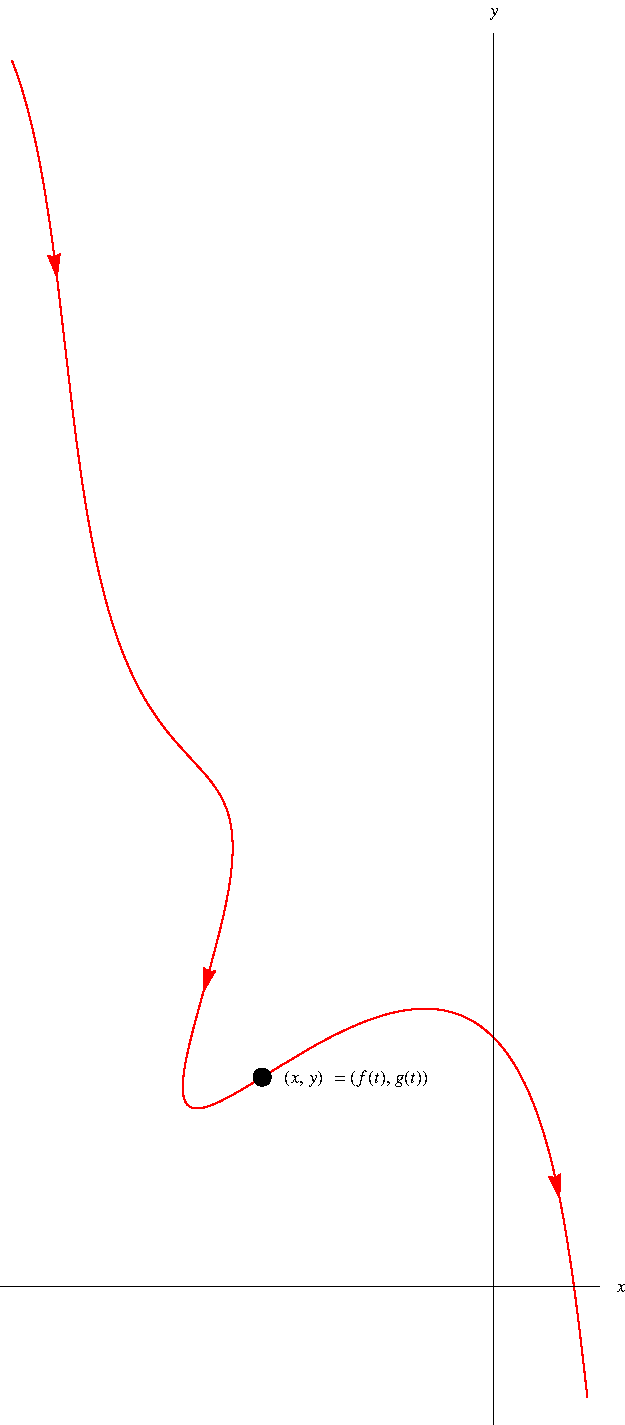
\includegraphics[height=4cm]{parametric-curves/pictures/11-01-parametricf.pdf}%
%}%
\column{.6\textwidth}
\begin{itemize}
\item  Suppose a particle moves along the curve in the picture.
\item<6->  The $x$-coordinate and $y$-coordinate of the particle are some functions of the time $t$.
\item<7->  We can write $x = f(t)$ and $y = g(t)$.
\item<8->  Less formally, we may directly write $(x,y)=(x(t), y(t))$.
\item<9->  We say that the equations $\left| \begin{array}{rcl}x &=& f(t)\\y&=&g(t)\end{array}\right.$ are parametric equations of a parametric curve.
\item<9->  Note that the curve can't be written as $y = f(x)$: it fails the vertical line test.
\end{itemize}
\end{columns}
\end{frame}
% end module parametric-intro

%%begin module parametric-curve-definition
\begin{frame}
%Let $[a,b]$ be an interval, and let $f_1, \dots, f_n$ be functions on the interval $[a,b]$. 
\begin{definition}[Curve in $n$-dimensional space]
We define an arbitrary $n$-tuple of functions $f_1,\dots, f_n$ on $[a,b]$ to be a \emph{parametric curve} (or simply \emph{curve}). If $\gamma$ is a curve, we write $\gamma$ as:
\[
\gamma:\left| 
\begin{array}{rcl}
x_1&=&f_1(t)\\
x_2&=&f_2(t)\\
&\vdots & \\
x_n&=&f_n(t)
\end{array} \right., t\in [a,b]\quad 
\]
where $x_1,\dots, x_n$ are the labels of the $n$-dimensional coordinate system.
\end{definition}
Curves in 2- and 3-dimensional space will be of special interest:
\begin{columns}
\column{0.5\textwidth}
A curve in dimension 2 is given by:
\[
\gamma:\left| 
\begin{array}{rcl}
x&=&f(t)\\
y&=&g(t)\\
\end{array} \right., t\in [a,b]\quad .
\]

\column{0.5\textwidth}
A curve in dimension 3 is given by:
\[
\gamma:\left| 
\begin{array}{rcl}
x&=&f(t)\\
y&=&g(t)\\
z&=&h(t)\\
\end{array} \right., t\in [a,b]\quad .
\]

\end{columns}

\end{frame}
%end module parametric-curve-definition
%%begin module curve-image-definition-intro
\begin{frame}
Consider the two parametric curves:
\begin{columns}
\column{0.5\textwidth}
\[
\gamma_1:
\left|
\begin{array}{rcl}
x&=&t^2\\
y&=&t^2\\
\end{array} \right., t\in [0,1]\quad
\]
\begin{center}
\psset{xunit=2cm, yunit=2cm}
\begin{pspicture}(-0.5, -0.5)(1.4,1.4)
\psframe*[linecolor=white](-0.5, -0.5)(1.400000,1.4)
\tiny
\fcAxesStandard{-0.200000}{-0.2}{1.2}{1.2}
\uncover<8->{
\psline[linecolor=\fcColorGraph](0,0)(1,1)
}
\uncover<2->{
\fcFullDot{0}{0}
}
\uncover<3->{
\fcFullDot{0.04}{0.04}
}
\uncover<4->{
\fcFullDot{0.16}{0.16}
}
\uncover<5->{
\fcFullDot{0.36}{0.36}
}
\uncover<6->{
\fcFullDot{0.64}{0.64}
}
\uncover<7->{
\fcFullDot{1}{1}
}
\end{pspicture}
\end{center}

\column{0.5\textwidth}
\[
\gamma_2:
\left|
\begin{array}{rcl}
x&=&t\\
y&=&t\\
\end{array} \right., t\in [0,1]\quad
\]
\begin{center}
\psset{xunit=2cm, yunit=2cm}
\begin{pspicture}(-0.5000000, -0.5)(1.400000,1.4)
\psframe*[linecolor=white](-0.5000000, -0.5)(1.400000,1.4)
\tiny
\fcAxesStandard{-0.200000}{-0.2}{1.2}{1.2}
\uncover<8->{
\psline[linecolor=\fcColorGraph ](0,0)(1,1)
}
\uncover<2->{
\fcFullDot{0}{0}
}
\uncover<3->{
\fcFullDot{0.2}{0.2}
}
\uncover<4->{
\fcFullDot{0.4}{0.4}
}
\uncover<5->{
\fcFullDot{0.6}{0.6}
}
\uncover<6->{
\fcFullDot{0.8}{0.8}
}
\uncover<7->{
\fcFullDot{1}{1}
}
\end{pspicture}
\end{center}
\end{columns}
\uncover<2->{Plug in} \uncover<2->{\alert<2>{$ t=0 $}}\uncover<3->{, \alert<3>{$t=0.2$}}\uncover<4->{, \alert<4>{$t = 0.4 $}}\uncover<5->{, \alert<5>{$t = 0.6$}}\uncover<6->{, \alert<6>{$t=0.8$}}\uncover<7->{, \alert<7>{$t = 1$}.}
\uncover<9->{
\begin{question}
Are the above curves different?
\end{question}
}
\uncover<10->{
To answer this question we need a definition.
}
\end{frame}
%end module curve-image-definition-intro

%
\begin{frame}
Recall a parametric curve $\gamma$  was defined as the data
\[
\gamma:
\left| 
\begin{array}{rcl}
x_1&=&f_1(t)\\
x_2&=&f_2(t)\\
&\vdots & \\
x_n&=&f_n(t)
\end{array} \right., t\in [a,b]\quad 
\]
\begin{definition}
A \emph{curve image} (or simply a curve) is any set of points that arises by traversing some \alert<2>{continuous} curve. In other words, a curve image is any set that can be written in the form
\[
\left\{(f_1(t),\dots, f_n(t))~|~ t\in [a,b]\right\}\quad ,
\]
for some \alert<2>{continuous} functions $f_1, \dots, f_n$.
\end{definition}
\only<2>{If we don't require that the functions be continuous, every set of points will be a curve and the definition would be pointless.}

\uncover<3->{Informally, a curve image ``remembers'' only the points lying on the curve but forgets the ``speed'' with which each point was visited and ``how many times'' each point was visited.
}
\end{frame}
%%begin module parametric-curve-vs-curve-image-terminology
\begin{frame}
\begin{columns}
\column{0.5\textwidth}
\begin{center}
\psset{xunit=1.5cm, yunit=1.5cm}
\begin{pspicture}(-1.000000, -5)(1.500000,5) 
\psframe*[linecolor=white](-1.000000,-5)(1.500000,5) 
\tiny 
\psaxesStandard{-0.200000}{-0.2}{1.2}{1.2}
\psline[linecolor=\psColorGraph](0,0)(1,1)
\rput[l](0.4,0.2){$C_1:
\left| 
\begin{array}{rcl}
x&=&t^2\\
y&=&t^2\\
\end{array} \right., t\in [0,1]
$}
\end{pspicture} 
\end{center}

\column{0.5\textwidth}
\begin{center}
\psset{xunit=1.5cm, yunit=1.5cm}
\begin{pspicture}(-1.000000, -5)(1.500000,5) 
\psframe*[linecolor=white](-1.000000,-5)(1.500000,5) 
\tiny 
\psaxesStandard{-0.200000}{-0.2}{1.2}{1.2}
\psline[linecolor=\psColorGraph ](0,0)(1,1)
\rput[l](0.4,0.2){$C_2:
\left| 
\begin{array}{rcl}
x&=&t\\
y&=&t\\
\end{array} \right., t\in [0,1]$
}
\end{pspicture}
\end{center}
\end{columns}
\begin{question}
$\begin{array}{l|l}
\only<1-3>{\text{ Are the above curves different?}}
\only<4->{\alert<4>{\xcancel{\text{ Are the above curves different?}}}} &\begin{array}{l} \uncover<2->{\alert<2>{\text{Are the above parametric curves} }
\\
\alert<2>{\text{different? Yes.}}}
\\
\uncover<3->{\alert<3>{\text{Are the above curve images}}\\ 
\alert<3>{\text{ different? No.}}}
\end{array}
\end{array}
$
\end{question}
\begin{itemize}
\only<1-4>{
\item<2-> As parametric curves, $C_1$ and $C_2$ are different: $C_1, C_2$ are given by different functions.
\item<3-> As curve images, $C_1,C_2$ coincide.
\item<4-> The original question is incorrectly posed: the word ``curve'' does not have a mathematical definition without the words ``parametric'' or ``image'' attached to it.
}
\item<5-> Nonetheless we sometimes use the word ``curve'' \alert<5>{informally}, without specifying ``parametric curve'' or ``curve image''. 
\item<6-> In this case, whether we mean  ``parametric curve'' or ``curve image'' should be clear from the context. \uncover<7->{\alert<7>{If not, we are using mathematical language incorrectly.}}
\end{itemize}

\vspace{5cm}

\end{frame}



%end module parametric-curve-vs-curve-image-terminology

%% begin module arc-length-intro
\begin{frame}
\frametitle{Arc Length}
\begin{center}

\psset{xunit=2cm, yunit=2cm}
\begin{pspicture}(-1, -1)(1,1)
\tiny %
\parametricplot[linecolor=\fcColorGraph, plotpoints=1000, algebraic=true]{0}{6.283185307}{cos(t)|sin(t)}%
\uncover<3>{ %
\fcRegularNgon[linecolor=\fcColorTangent]{3}{1}%
}
\uncover<4>{ %
\fcRegularNgon[linecolor=\fcColorTangent]{4}{1}%
}
\uncover<5>{ %
\fcRegularNgon[linecolor=\fcColorTangent]{6}{1}%
}
\uncover<6>{ %
\fcRegularNgon[linecolor=\fcColorTangent]{8}{1}%
}
\uncover<7>{ %
\fcRegularNgon[linecolor=\fcColorTangent]{12}{1}%
}
\uncover<8>{ %
\fcRegularNgon[linecolor=\fcColorTangent]{16}{1}%
}
\uncover<9>{ %
\fcRegularNgon[linecolor=\fcColorTangent]{32}{1}%
}
\end{pspicture}

\uncover<1-9>{}
%\ \only<-2>{%
%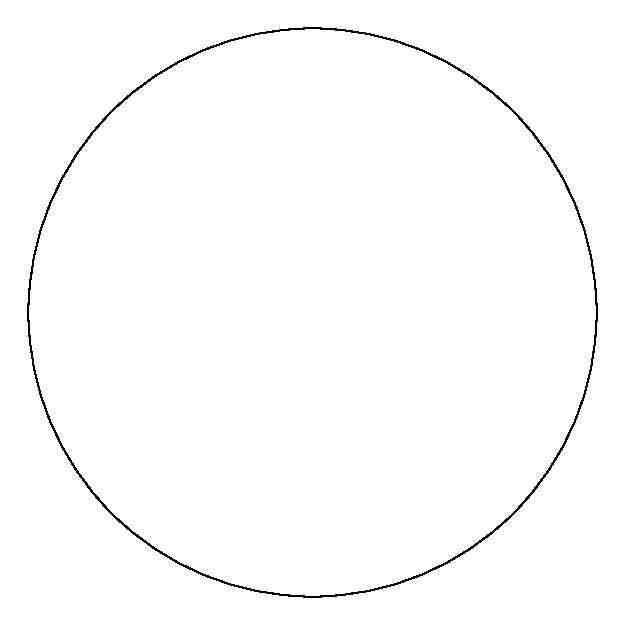
\includegraphics[height=4cm]{arc-length/pictures/09-01-circlea.pdf}%
%}%
%\only<handout:0| 3>{%
%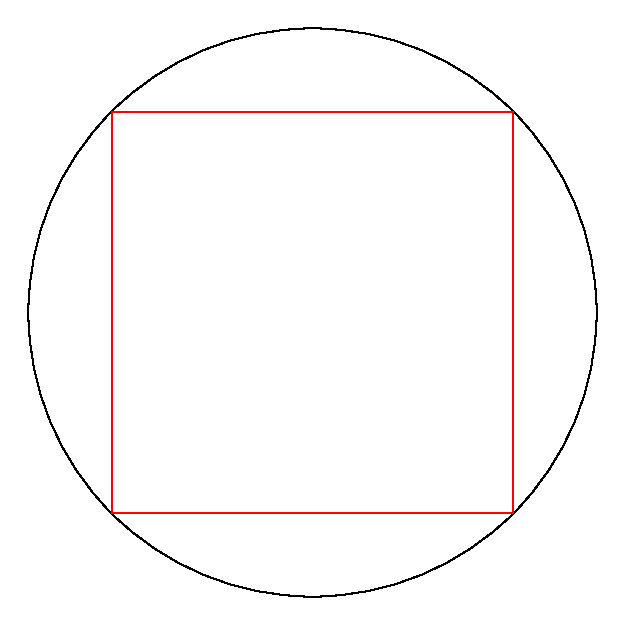
\includegraphics[height=4cm]{arc-length/pictures/09-01-circleb.pdf}%
%}%
%\only<handout:0| 4>{%
%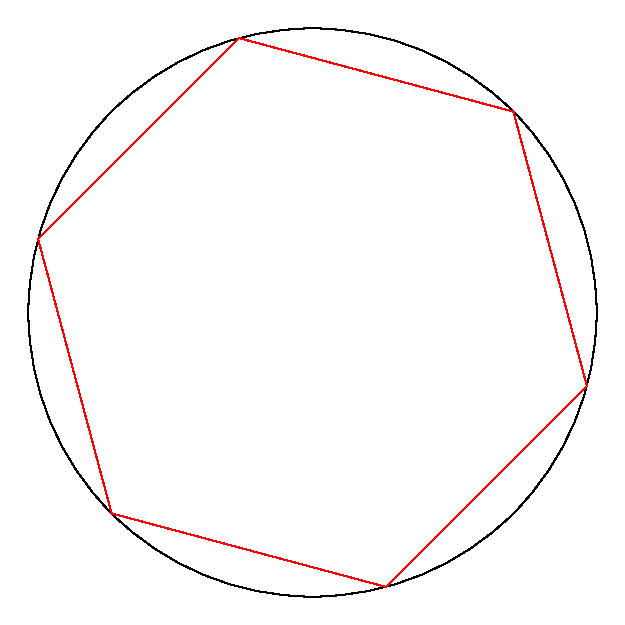
\includegraphics[height=4cm]{arc-length/pictures/09-01-circlec.pdf}%
%}%
%\only<handout:0| 5>{%
%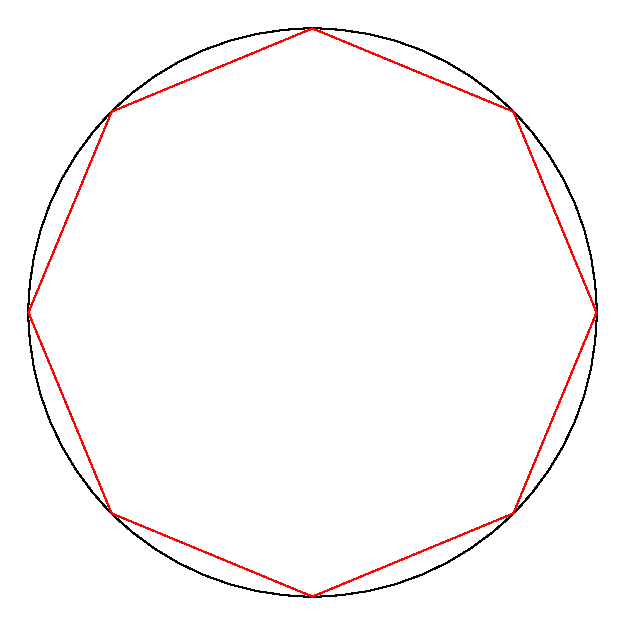
\includegraphics[height=4cm]{arc-length/pictures/09-01-circled.pdf}%
%}%
%\only<handout:0| 6>{%
%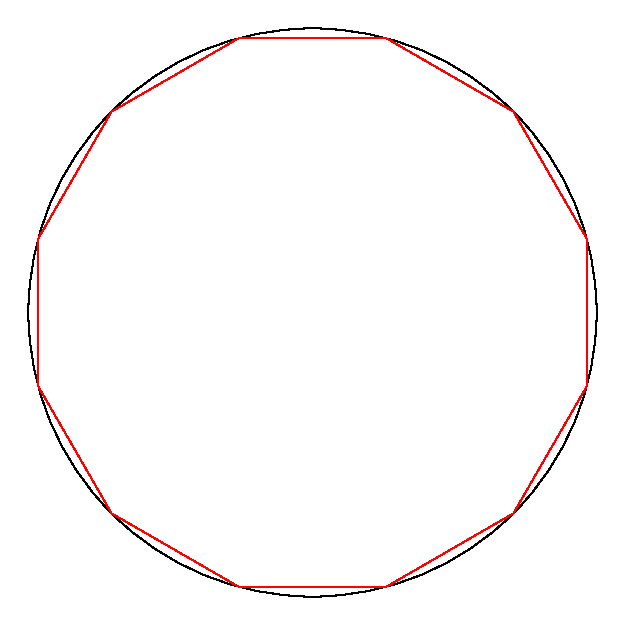
\includegraphics[height=4cm]{arc-length/pictures/09-01-circlee.pdf}%
%}%
%\only<handout:0| 7->{%
%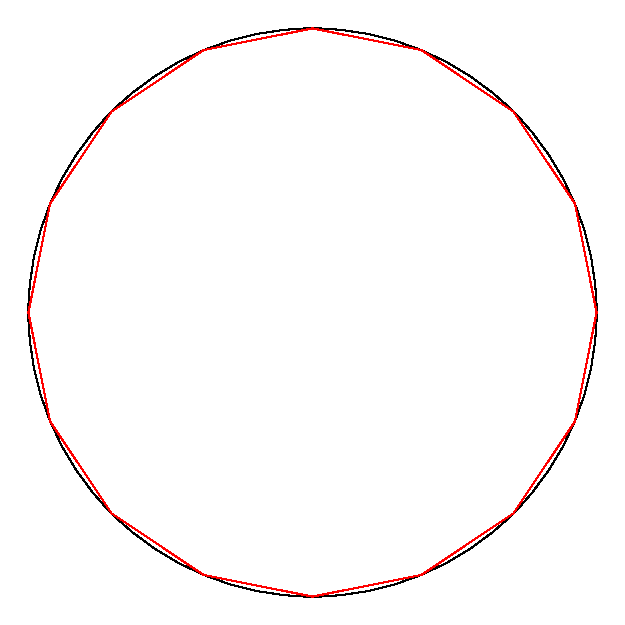
\includegraphics[height=4cm]{arc-length/pictures/09-01-circlef.pdf}%
%}%
\end{center}
\begin{itemize}
\item  What do we mean by the length of a curve?
\item<2->  The length of a polygon is easy to compute: add up the length of the line segments that form the polygon.
\item<3->  If the curve is a circle, approximate it by a polygon.
\item<4->  Then take the limit as the number of segments of the polygon goes to $\infty$.
\end{itemize}
\end{frame}
% end module arc-length-intro

%%begin module arc-length-derivation-parametric
{% scoping block for the following command:
%Calculator input: plotCurve{}(t, 8 t^{4}-40 t^{3}+70 t^{2}-50 t+13, 2/5, 2)
\newcommand{\theCurve}{t 13 t -50 mul add t 2 exp 70 mul add t 3 exp -40 mul add t 4 exp 8 mul add}
\newcommand{\lowBound}{0.4}
\newcommand{\highBound}{2}
\begin{frame}
Let $\gamma $ be the curve
$ \gamma: \left|
\begin{array}{rcl}
x=x(t)\\
y=y(t)
\end{array}, t\in [a,b]
\right.$

\begin{itemize}
\item<2->  Divide $[a,b]$ into $n$ subintervals with endpoints $t_0, t_1, \ldots , t_n$ and equal width $\Delta t$.
\item<3->  The points $P_i = (x(t_i), y(t_i))$ lie on the curve $\gamma$. The lengths of the segments with endpoints with consecutive indices from $P_0, P_1, \ldots , P_n$ approximate the length of the curve $\gamma$.
\item<4->  The length $L$ of the curve $\gamma$ is the limit of the lengths of these segments as $n\rightarrow \infty$.
\end{itemize}
\begin{columns}[c]
\column{.6\textwidth}
\begin{center}
\psset{xunit=1.4cm, yunit=1.4cm}
\begin{pspicture}(-0.4,-0.3)(2.3,1.994800)
\tiny
\fcAxesStandard{-0.3}{-0.3}{2.146803}{1.994800}
%\theCurve is defined in the beginning of this module, has limited scope
\parametricplot{\lowBound}{\highBound}{\theCurve}
\uncover<2-4>{%
\fcPolylineAlongCurveWithLabels[linecolor=\fcColorGraph]{3}{\lowBound}{\highBound}{\theCurve}{P}%
}
\uncover<5>{%
\fcPolylineAlongCurveWithLabels[linecolor=\fcColorGraph]{4}{\lowBound}{\highBound}{\theCurve}{P}%
}
\uncover<6>{%
\fcPolylineAlongCurveWithLabels[linecolor=\fcColorGraph]{5}{\lowBound}{\highBound}{\theCurve}{P}%
}
\uncover<7>{%
\fcPolylineAlongCurveWithLabels[linecolor=\fcColorGraph]{6}{\lowBound}{\highBound}{\theCurve}{P}%
}
\uncover<8>{%
\fcPolylineAlongCurveWithLabels[linecolor=\fcColorGraph]{10}{\lowBound}{\highBound}{\theCurve}{P}%
}
\uncover<9->{%0
\fcPolylineAlongCurveWithLabels[linecolor=\fcColorGraph]{14}{\lowBound}{\highBound}{\theCurve}{P}%
}
\end{pspicture}
%\ \only<handout:0| -1>{%
%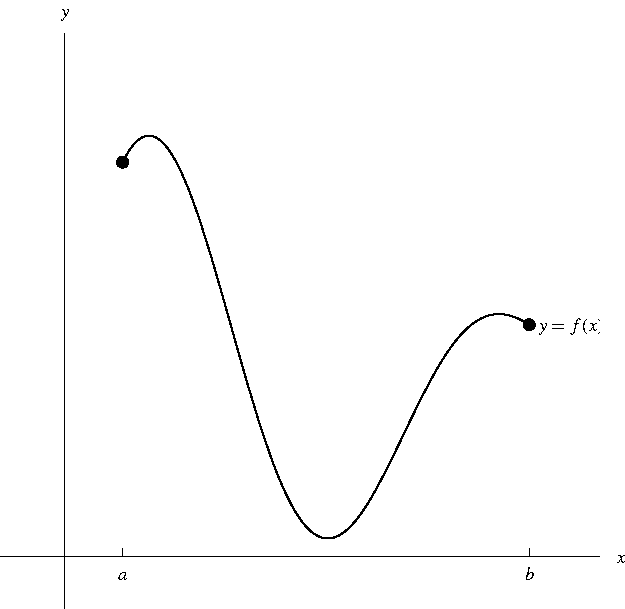
\includegraphics[height=4.5cm]{arc-length/pictures/09-01-arclengtha.pdf}%
%}%
%\only<handout:0| 2-4>{%
%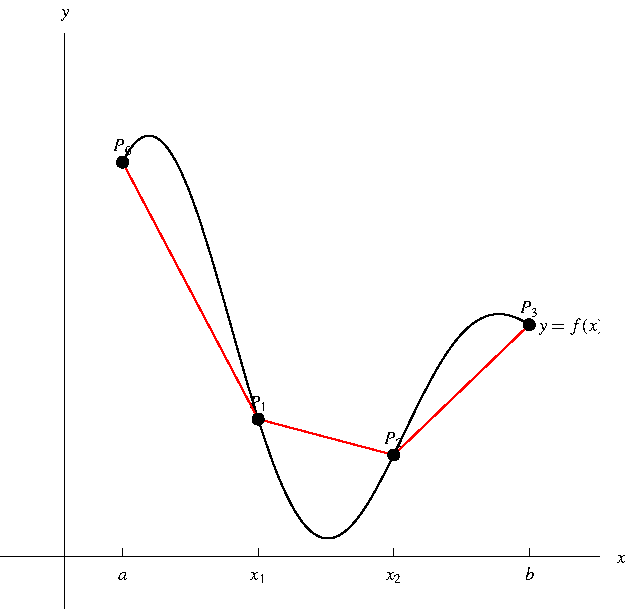
\includegraphics[height=4.5cm]{arc-length/pictures/09-01-arclengthb.pdf}%
%}%
%\only<handout:0| 5>{%
%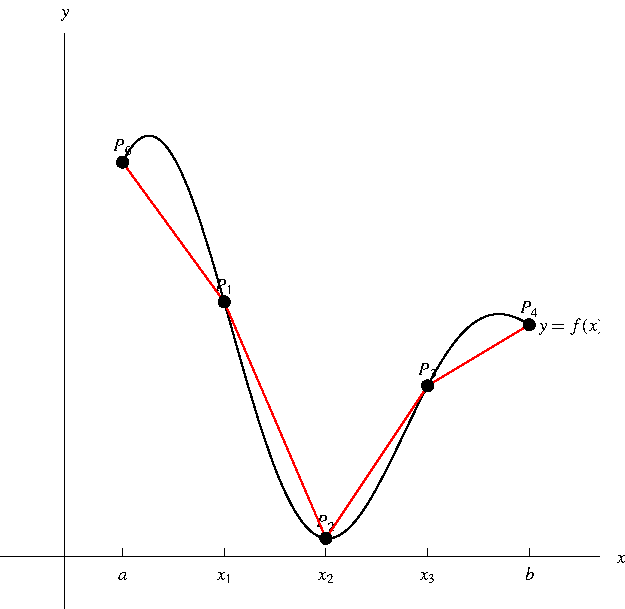
\includegraphics[height=4.5cm]{arc-length/pictures/09-01-arclengthc.pdf}%
%}%
%\only<handout:0| 6>{%
%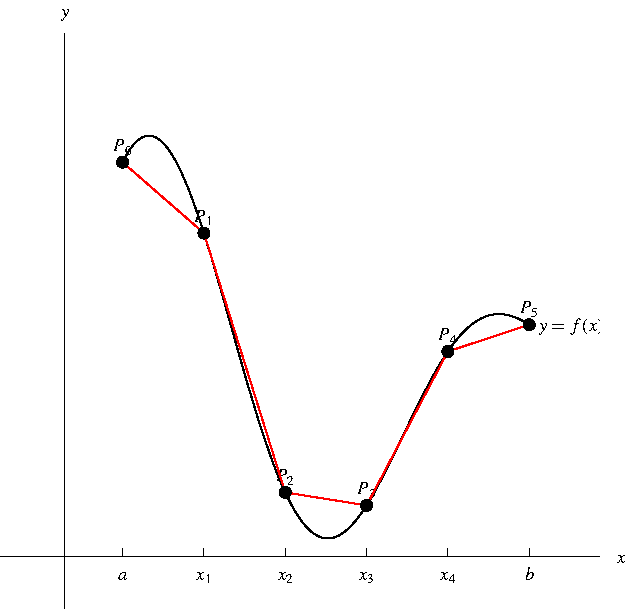
\includegraphics[height=4.5cm]{arc-length/pictures/09-01-arclengthd.pdf}%
%}%
%\only<handout:0| 7>{%
%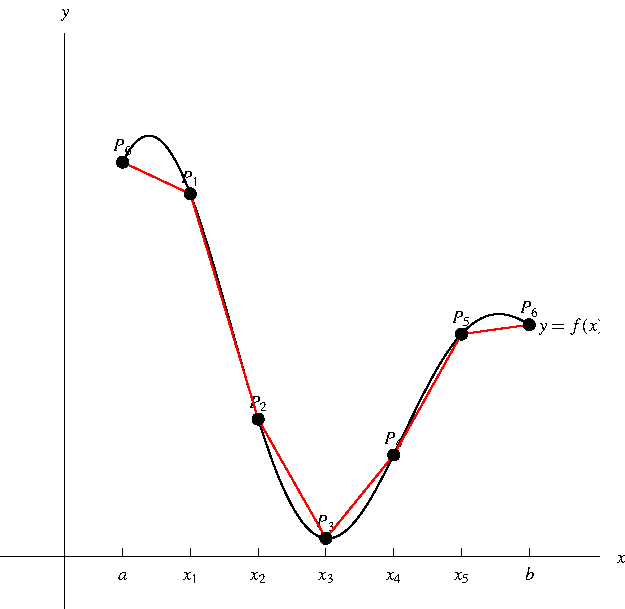
\includegraphics[height=4.5cm]{arc-length/pictures/09-01-arclengthe.pdf}%
%}%
%\only<8>{%
%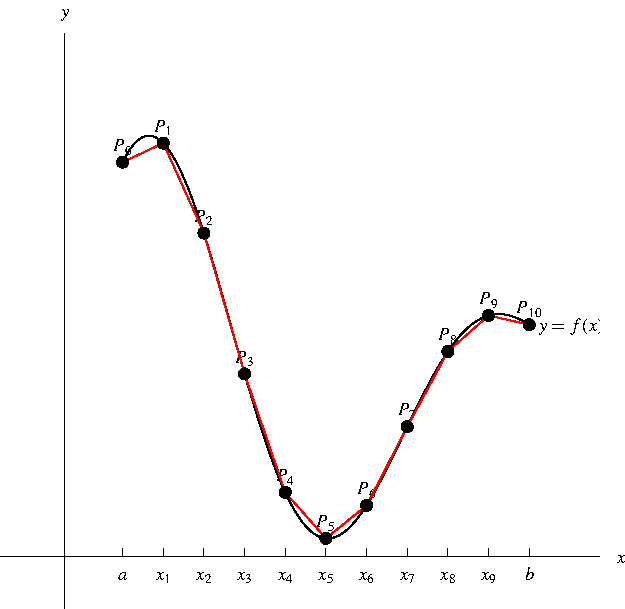
\includegraphics[height=4.5cm]{arc-length/pictures/09-01-arclengthf.pdf}%
%}%
%\only<handout:0| 9->{%
%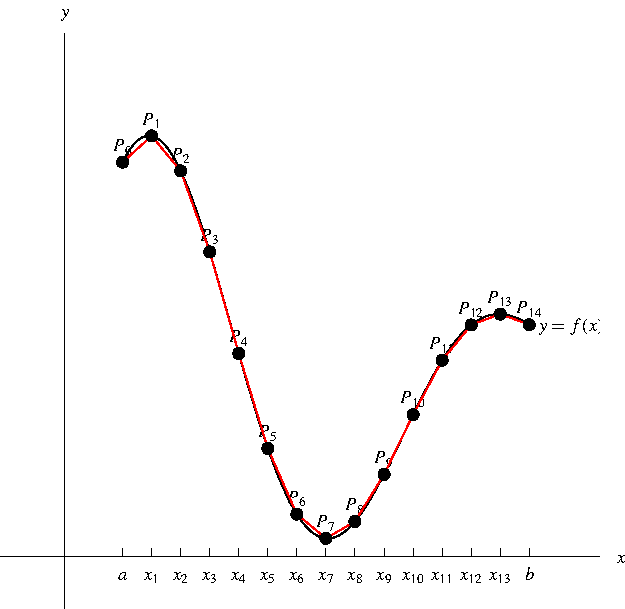
\includegraphics[height=4.5cm]{arc-length/pictures/09-01-arclengthg.pdf}%
%}%
%\only<10->{%
%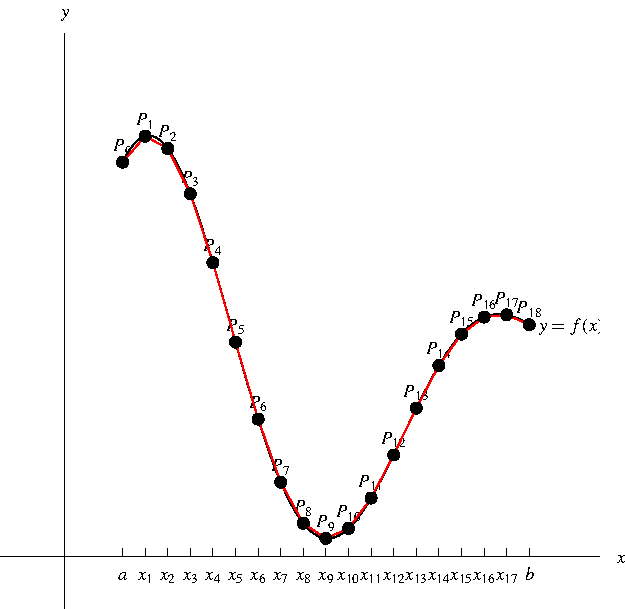
\includegraphics[height=4.5cm]{arc-length/pictures/09-01-arclengthh.pdf}%
%}%
\end{center}
\column{.4\textwidth}
\uncover<10->{%
\[
L = \lim_{n\rightarrow \infty} \sum_{i=1}^n |P_{i-1}P_i|
\]
}%
\end{columns}
\end{frame}



\begin{frame}
Let $\gamma $ be the curve
$ \gamma: \left|
\begin{array}{rcl}
x=x(t)\\
y=y(t)
\end{array}, t\in [a,b]
\right.$

$\begin{array}{rcl}
\uncover<1->{%
L = \lim_{n\rightarrow \infty} \sum_{i = 1}^n \alert<handout:0| 10>{|P_{i-1}P_i|}%
}%
& \uncover<10->{ = } &%
\uncover<10->{%
\alert<handout:0| 12>{\lim_{n\rightarrow\infty} \sum_{i=1}^n} \alert<handout:0| 10>{\sqrt{\alert<handout:0|13>{ (x'(s_i))^2}+\alert<handout:0| 13>{(y'(r_i))^2}}\ \alert<handout:0| 14>{\Delta t}}%
}\\%
& \uncover<11->{ = } &%
\uncover<11->{%
\alert<handout:0| 12>{\int_a^b} \sqrt{ \alert<handout:0| 13>{(x'(t))^2} +\alert<handout:0| 13>{(y'(t))^2}} \ \alert<handout:0| 14>{\diff t}%
}%
\end{array}
$
\begin{itemize}
\item If $f$ has continuous derivative, we can compute the above limit.
\item<2-> Let 
$\left|\begin{array}{r@{~}c@{~}l} 
x_i &=& x(t_i)\\ 
y_i &=& y(t_i)
\end{array}\right.$, 
and 
$\left|\begin{array}{rcl}
\Delta x &=& x_i - x_{i-1} = x(t_i) - x(t_{i-1})\\ 
\Delta y &=& y_i - y_{i-1} = y(t_i) - y(t_{i-1}) 
\end{array}\right. $.
\item<3-| alert@6> Then $|P_iP_{i-1}| = \sqrt{(\Delta x)^2 + (\Delta y)^2}$.
\item<4-> Mean Value Theorem: there exist numbers $s_i$ and $r_i$ between $t_{i-1}$ and $t_i$ such that $\alert<handout:0| 5>{x(t_i) - x(t_{i-1}) = x'(s_i )(t_i- t_{i-1})}$  and $\alert<handout:0| 5>{y(t_i) - y(t_{i-1}) = y'(r_i)( t_i-t_{i-1})}$
\item<5-| alert@5,7> $\Delta x = x'(s_i)\Delta t$, $\Delta y = y'(r_i)\Delta t$.
\end{itemize}
$\begin{array}{rcl}
\uncover<6->{%
\alert<handout:0| 10>{|P_{i-1}P_i|}%
}%
& \uncover<6->{\alert<handout:0| 10>{ = }} &%
\uncover<6->{%
\sqrt{(\alert<handout:0| 7>{\Delta x})^2 + (\alert<handout:0| 7>{\Delta y})^2}%
}  \uncover<7->{ = } \uncover<7->{%
\sqrt{ (\alert<handout:0| 7>{x'(s_i)\Delta t})^2 + (\alert<handout:0| 7>{y'(r_i)\Delta t})^2}%
}\\%
& \uncover<8->{ = } &%
\uncover<8->{%
\sqrt{(x'(s_i))^2 + (y'(r_i))^2}\sqrt{(\Delta t)^2}%
}  \uncover<9->{ = } \uncover<9->{%
\alert<handout:0| 10>{\sqrt{(x'(s_i))^2 + (y'(r_i))^2}\ \Delta t }%
}\\%
\end{array}
$
\end{frame}
}% end of scoping block
%end module arc-length-derivation-parametric

%% begin module arc-length-derivation
\begin{frame}
\begin{itemize}
\item  What about $y = f(x)$ for a continuous function $f$ on $[a, b]$?
\item<2->  Divide $[a,b]$ into $n$ subintervals with endpoints $x_0, x_1, \ldots , x_n$ and equal width $\Delta x$.
\item<3->  The points $P_i = (x_i, f(x_i))$ lie on $y = f(x)$, and the segments with vertices $P_0, P_1, \ldots , P_n$ are an approximation to $y = f(x)$.
\item<4->  The length $L$ of the curve $y = f(x)$ is the limit of the lengths of these segments as $n\rightarrow \infty$.
\end{itemize}
\begin{columns}[c]
\column{.6\textwidth}
\begin{center}
\ \only<handout:0| -1>{%
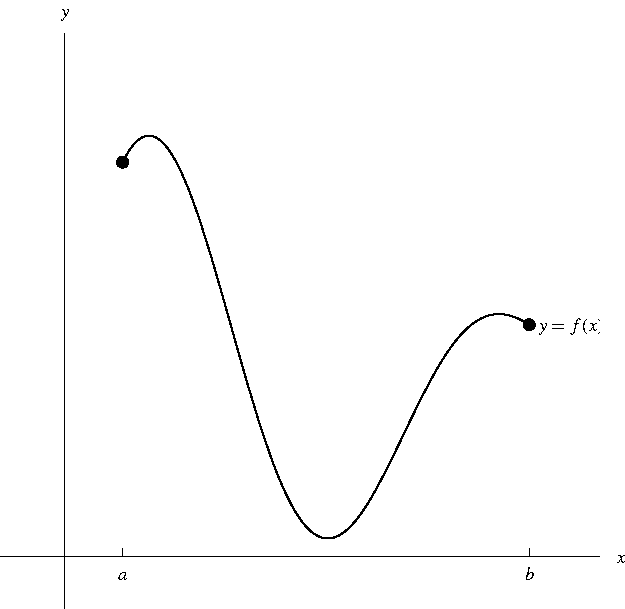
\includegraphics[height=4.5cm]{arc-length/pictures/09-01-arclengtha.pdf}%
}%
\only<handout:0| 2-4>{%
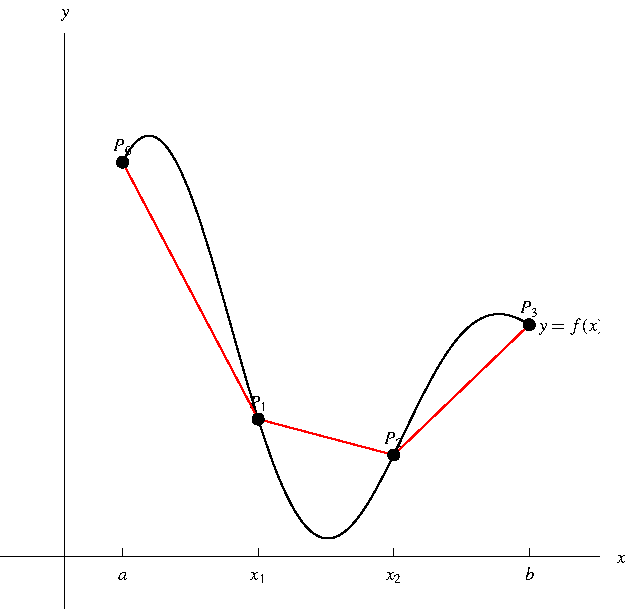
\includegraphics[height=4.5cm]{arc-length/pictures/09-01-arclengthb.pdf}%
}%
\only<handout:0| 5>{%
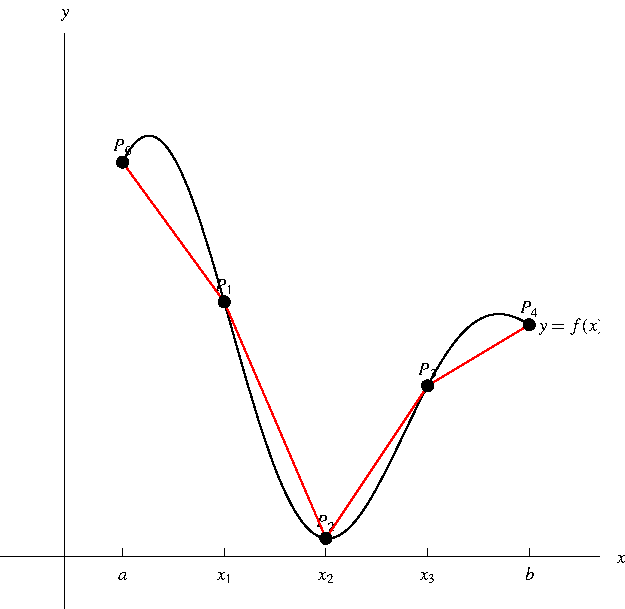
\includegraphics[height=4.5cm]{arc-length/pictures/09-01-arclengthc.pdf}%
}%
\only<handout:0| 6>{%
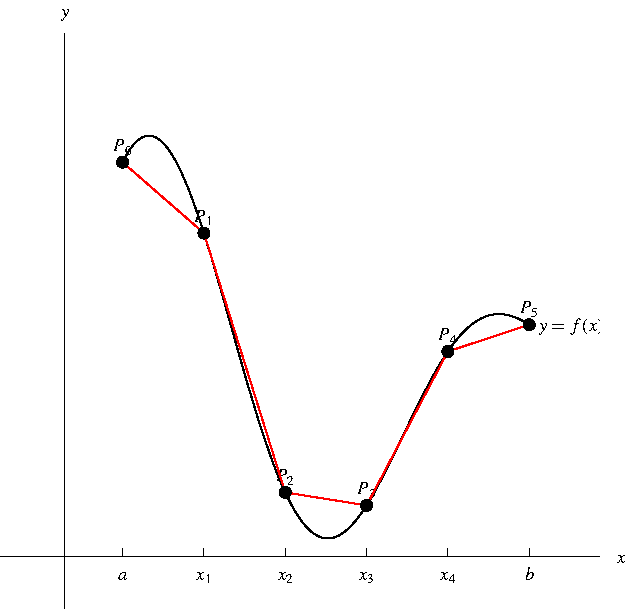
\includegraphics[height=4.5cm]{arc-length/pictures/09-01-arclengthd.pdf}%
}%
\only<handout:0| 7>{%
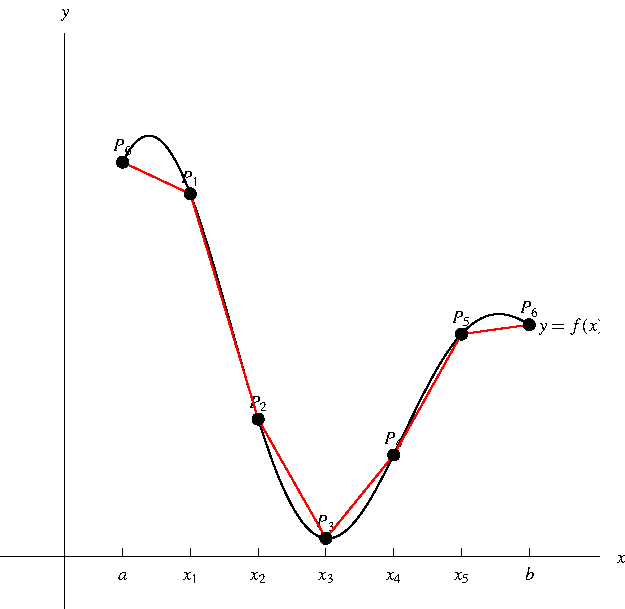
\includegraphics[height=4.5cm]{arc-length/pictures/09-01-arclengthe.pdf}%
}%
\only<8>{%
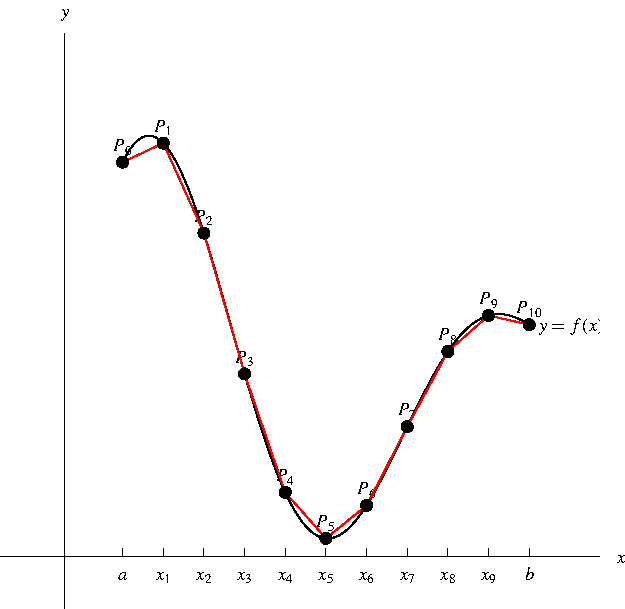
\includegraphics[height=4.5cm]{arc-length/pictures/09-01-arclengthf.pdf}%
}%
\only<handout:0| 9->{%
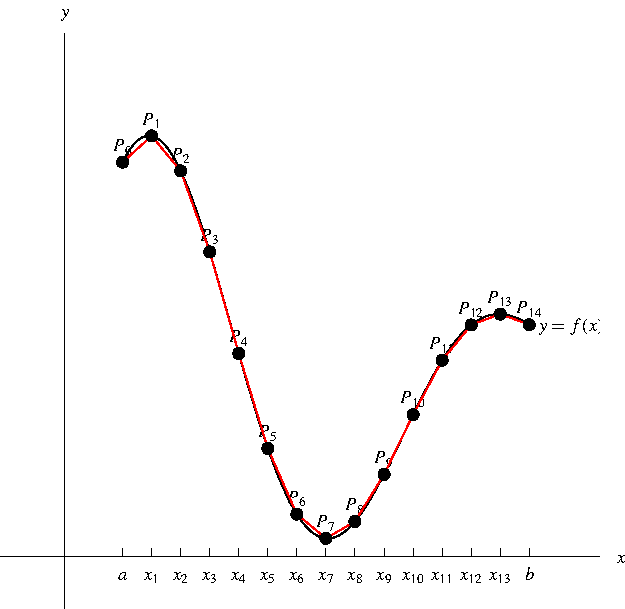
\includegraphics[height=4.5cm]{arc-length/pictures/09-01-arclengthg.pdf}%
}%
%\only<10->{%
%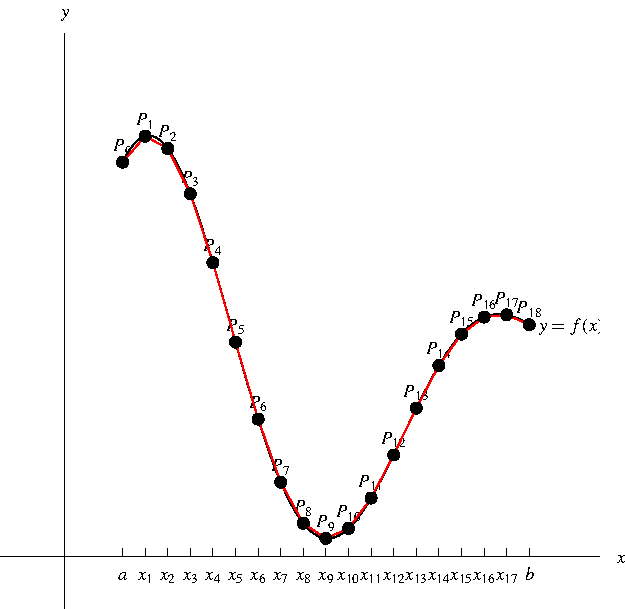
\includegraphics[height=4.5cm]{arc-length/pictures/09-01-arclengthh.pdf}%
%}%
\end{center}
\column{.4\textwidth}
\uncover<10->{%
\[
L = \lim_{n\rightarrow \infty} \sum_{i=1}^n |P_{i-1}P_i|
\]
}%
\end{columns}
\end{frame}



\begin{frame}
\begin{eqnarray*}
\uncover<1->{%
L = \lim_{n\rightarrow \infty} \sum_{i = 1}^n \alertNoH{ 10}{|P_{i-1}P_i|}%
}%
& \uncover<10->{ = } &%
\uncover<10->{%
\alertNoH{ 12}{\lim_{n\rightarrow\infty} \sum_{i=1}^n} \alertNoH{ 10}{\sqrt{1+\alertNoH{ 13}{(f'(x_i^*))^2}}\ \alertNoH{ 14}{\Delta x}}%
}\\%
& \uncover<11->{ = } &%
\uncover<11->{%
\alertNoH{ 12}{\int_a^b} \sqrt{1+\alertNoH{ 13}{(f'(x))^2}} \ \alertNoH{ 14}{\diff x}%
}%
\end{eqnarray*}
\begin{itemize}
\item  This formula is not useful for computational purposes.
\item  We can find a better formula when $f$ has a continuous derivative.
\item<2->  Let $y_i = f(x_i)$, and $\Delta y = y_i - y_{i-1} = f(x_i) - f(x_{i-1})$.
\item<3-| alert@6>  Then $|P_iP_{i-1}| = \sqrt{(x_i-x_{i-1})^2+(y_i-y_{i-1})^2} = \sqrt{(\Delta x)^2 + (\Delta y)^2}$.
\item<4->  Mean Value Theorem: there exists $x_i^*$ between $x_{i-1}$ and $x_i$ such that $\alertNoH{ 5}{f(x_i) - f(x_{i-1}) = f'(x_i^*)(x_i-x_{i-1})}$.
\item<5-| alert@5,7>  $\Delta y = f'(x_i^*)\Delta x$.
\end{itemize}
\begin{eqnarray*}
\uncover<6->{%
\alertNoH{ 10}{|P_{i-1}P_i|}%
}%
& \uncover<6->{\alertNoH{ 10}{ = }} &%
\uncover<6->{%
\sqrt{(\Delta x)^2 + (\alertNoH{ 7}{\Delta y})^2}%
}  \uncover<7->{ = } \uncover<7->{%
\sqrt{(\Delta x)^2 + (\alertNoH{ 7}{f'(x_i^*)\Delta x})^2}%
}\\%
& \uncover<8->{ = } &%
\uncover<8->{%
\sqrt{1 + (f'(x_i^*))^2}\sqrt{(\Delta x)^2}%
}  \uncover<9->{ = } \uncover<9->{%
\alertNoH{ 10}{\sqrt{1 + (f'(x_i^*))^2}\ \Delta x}%
}\\%
\end{eqnarray*}
\end{frame}
% end module arc-length-derivation

%% begin module arc-length-def
\begin{frame}
\frametitle{The Arc Length Formula}
Let $\gamma:\left|\begin{array}{rcl} x&=&x(t)\\ y&=&y(t)\end{array}  \right., t\in [a,b]$.


\begin{definition}
Suppose $x'(t)$ and $y'(t)$ (exist and) are continuous on $[a,b]$. Then the length of the curve $\gamma$ is defined as 
\[
\begin{array}{rclll}
\displaystyle L(\gamma) &=&\displaystyle  \int_a^b \sqrt{(x'(t))^2 +(y'(t))^2} ~ \diff x\\
\uncover<2->{&=& \displaystyle \int_a^b \sqrt{\left(\frac{\diff x}{\diff t}\right)^2 + \left( \frac{\diff y}{\diff t}\right)^2} ~ \diff t &&\text{in Leibniz notation .}}
\end{array}
\]

\end{definition}
\end{frame}
% end module arc-length-def

%%begin module graphs-of-functions-as-curves
\begin{frame}
\frametitle{Graphs of functions as curve images}
\begin{itemize}
\item Consider a graph of a function given by 
\[
y=f(x)
\]
\item<2-> Write $\alert<3>{x=t}$. Then $y=f(x)\uncover<3->{ =f(\alert<3>{t})}$\uncover<4->{, so we get the system }
\uncover<4->{
\[
C: \left|\begin{array}{rcl}
x&=&t\\
y&=&f(t)
\end{array}\right., t\in [a,b]
\]
}
\end{itemize}
\uncover<5->{
\begin{observation}
The graph of an arbitrary function can be written as the image of a curve $C$ using the above transformation.
\end{observation}
}
\end{frame}

%end module graphs-of-functions-as-curves

%%begin module arc-length-function-graph-from-parametric-curve-length

\begin{frame}
\frametitle{Arc length of graph of a function}
\begin{question}
What is the length of the graph of the curve given by the graph of $y=f(x)$?
\end{question}
\begin{itemize}
\item<2-> The graph of $y=f(x)$ is written as a curve as 
\[
\gamma:\left|
\begin{array}{rcl}
\alertNoH{7}{x}&\alertNoH{7}{=}&\alertNoH{7}{t}\\
y&\alertNoH{0}{=}&f(t) 
\end{array}\right.,t\in [a,b]\quad .
\]
\item<3-> In other words, the question asks what is the length $L(\gamma)$ of $\gamma$. \uncover<4->{That is a straightforward computation: 
$
\begin{array}{rcl}
\uncover<4->{L(\gamma)}&\uncover<4->{=}&
\displaystyle \int \sqrt{( \alertNoH{6,7}{x'(t)})^2 +(\alertNoH{5}{y'(t)})^2 } \diff t= \uncover<5->{\int \sqrt{ \fcAnswerUncover{5}{7}{1} +(\alertNoH{5}{f'(t)})^2 } \diff t }
\end{array}
$
}
\end{itemize}

\end{frame}
%end module arc-length-function-graph-from-parametric-curve-length
%%begin module arc-length-does-not-depend-on-parametrization-when-one-to-one

%end module arc-length-does-not-depend-on-parametrization-when-one-to-one
%% begin module arc-length-def
\begin{frame}
\frametitle{The Arc Length Formula}
Let $\gamma:\left|\begin{array}{rcl} x&=&x(t)\\ y&=&y(t)\end{array}  \right., t\in [a,b]$.


\begin{definition}
Suppose $x'(t)$ and $y'(t)$ (exist and) are continuous on $[a,b]$. Then the length of the curve $\gamma$ is defined as 
\[
\begin{array}{rclll}
\displaystyle L(\gamma) &=&\displaystyle  \int_a^b \sqrt{(x'(t))^2 +(y'(t))^2} ~ \diff x\\
\uncover<2->{&=& \displaystyle \int_a^b \sqrt{\left(\frac{\diff x}{\diff t}\right)^2 + \left( \frac{\diff y}{\diff t}\right)^2} ~ \diff t &&\text{in Leibniz notation .}}
\end{array}
\]

\end{definition}
\end{frame}
% end module arc-length-def

%% begin module arc-length-def
\begin{frame}
\frametitle{The Arc Length Formula}

\begin{definition}
Suppose $f'$ exists and is continuous on $[a,b]$. Then the length of the curve $y = f(x)$, $a\leq x \leq b$, is
\[
\begin{array}{rclll}
\displaystyle L& =&\displaystyle  \int\limits_a^b \sqrt{1 +( f' (x))^2} \ \diff x\\
 &=&\displaystyle  \int\limits_a^b \sqrt{1 + \left( \frac{\diff y}{\diff x}\right)^2} \ \diff x&&\text{(in Leibniz notation)\quad .}
\end{array}
\]
\end{definition}

\end{frame}
% end module arc-length-def

%%begin module parametric-curve-definition
\begin{frame}
%Let $[a,b]$ be an interval, and let $f_1, \dots, f_n$ be functions on the interval $[a,b]$. 
\begin{definition}[Curve in $n$-dimensional space]
We define an arbitrary $n$-tuple of functions $f_1,\dots, f_n$ on $[a,b]$ to be a \emph{parametric curve} (or simply \emph{curve}). If $\gamma$ is a curve, we write $\gamma$ as:
\[
\gamma:\left| 
\begin{array}{rcl}
x_1&=&f_1(t)\\
x_2&=&f_2(t)\\
&\vdots & \\
x_n&=&f_n(t)
\end{array} \right., t\in [a,b]\quad 
\]
where $x_1,\dots, x_n$ are the labels of the $n$-dimensional coordinate system.
\end{definition}
Curves in 2- and 3-dimensional space will be of special interest:
\begin{columns}
\column{0.5\textwidth}
A curve in dimension 2 is given by:
\[
\gamma:\left| 
\begin{array}{rcl}
x&=&f(t)\\
y&=&g(t)\\
\end{array} \right., t\in [a,b]\quad .
\]

\column{0.5\textwidth}
A curve in dimension 3 is given by:
\[
\gamma:\left| 
\begin{array}{rcl}
x&=&f(t)\\
y&=&g(t)\\
z&=&h(t)\\
\end{array} \right., t\in [a,b]\quad .
\]

\end{columns}

\end{frame}
%end module parametric-curve-definition
%%begin module curve-image-definition-intro
\begin{frame}
Consider the two parametric curves:
\begin{columns}
\column{0.5\textwidth}
\[
\gamma_1:
\left|
\begin{array}{rcl}
x&=&t^2\\
y&=&t^2\\
\end{array} \right., t\in [0,1]\quad
\]
\begin{center}
\psset{xunit=2cm, yunit=2cm}
\begin{pspicture}(-0.5, -0.5)(1.4,1.4)
\psframe*[linecolor=white](-0.5, -0.5)(1.400000,1.4)
\tiny
\fcAxesStandard{-0.200000}{-0.2}{1.2}{1.2}
\uncover<8->{
\psline[linecolor=\fcColorGraph](0,0)(1,1)
}
\uncover<2->{
\fcFullDot{0}{0}
}
\uncover<3->{
\fcFullDot{0.04}{0.04}
}
\uncover<4->{
\fcFullDot{0.16}{0.16}
}
\uncover<5->{
\fcFullDot{0.36}{0.36}
}
\uncover<6->{
\fcFullDot{0.64}{0.64}
}
\uncover<7->{
\fcFullDot{1}{1}
}
\end{pspicture}
\end{center}

\column{0.5\textwidth}
\[
\gamma_2:
\left|
\begin{array}{rcl}
x&=&t\\
y&=&t\\
\end{array} \right., t\in [0,1]\quad
\]
\begin{center}
\psset{xunit=2cm, yunit=2cm}
\begin{pspicture}(-0.5000000, -0.5)(1.400000,1.4)
\psframe*[linecolor=white](-0.5000000, -0.5)(1.400000,1.4)
\tiny
\fcAxesStandard{-0.200000}{-0.2}{1.2}{1.2}
\uncover<8->{
\psline[linecolor=\fcColorGraph ](0,0)(1,1)
}
\uncover<2->{
\fcFullDot{0}{0}
}
\uncover<3->{
\fcFullDot{0.2}{0.2}
}
\uncover<4->{
\fcFullDot{0.4}{0.4}
}
\uncover<5->{
\fcFullDot{0.6}{0.6}
}
\uncover<6->{
\fcFullDot{0.8}{0.8}
}
\uncover<7->{
\fcFullDot{1}{1}
}
\end{pspicture}
\end{center}
\end{columns}
\uncover<2->{Plug in} \uncover<2->{\alert<2>{$ t=0 $}}\uncover<3->{, \alert<3>{$t=0.2$}}\uncover<4->{, \alert<4>{$t = 0.4 $}}\uncover<5->{, \alert<5>{$t = 0.6$}}\uncover<6->{, \alert<6>{$t=0.8$}}\uncover<7->{, \alert<7>{$t = 1$}.}
\uncover<9->{
\begin{question}
Are the above curves different?
\end{question}
}
\uncover<10->{
To answer this question we need a definition.
}
\end{frame}
%end module curve-image-definition-intro

%
\begin{frame}
Recall a parametric curve $\gamma$  was defined as the data
\[
\gamma:
\left| 
\begin{array}{rcl}
x_1&=&f_1(t)\\
x_2&=&f_2(t)\\
&\vdots & \\
x_n&=&f_n(t)
\end{array} \right., t\in [a,b]\quad 
\]
\begin{definition}
A \emph{curve image} (or simply a curve) is any set of points that arises by traversing some \alert<2>{continuous} curve. In other words, a curve image is any set that can be written in the form
\[
\left\{(f_1(t),\dots, f_n(t))~|~ t\in [a,b]\right\}\quad ,
\]
for some \alert<2>{continuous} functions $f_1, \dots, f_n$.
\end{definition}
\only<2>{If we don't require that the functions be continuous, every set of points will be a curve and the definition would be pointless.}

\uncover<3->{Informally, a curve image ``remembers'' only the points lying on the curve but forgets the ``speed'' with which each point was visited and ``how many times'' each point was visited.
}
\end{frame}
%%begin module parametric-curve-vs-curve-image-terminology
\begin{frame}
\begin{columns}
\column{0.5\textwidth}
\begin{center}
\psset{xunit=1.5cm, yunit=1.5cm}
\begin{pspicture}(-1.000000, -5)(1.500000,5) 
\psframe*[linecolor=white](-1.000000,-5)(1.500000,5) 
\tiny 
\psaxesStandard{-0.200000}{-0.2}{1.2}{1.2}
\psline[linecolor=\psColorGraph](0,0)(1,1)
\rput[l](0.4,0.2){$C_1:
\left| 
\begin{array}{rcl}
x&=&t^2\\
y&=&t^2\\
\end{array} \right., t\in [0,1]
$}
\end{pspicture} 
\end{center}

\column{0.5\textwidth}
\begin{center}
\psset{xunit=1.5cm, yunit=1.5cm}
\begin{pspicture}(-1.000000, -5)(1.500000,5) 
\psframe*[linecolor=white](-1.000000,-5)(1.500000,5) 
\tiny 
\psaxesStandard{-0.200000}{-0.2}{1.2}{1.2}
\psline[linecolor=\psColorGraph ](0,0)(1,1)
\rput[l](0.4,0.2){$C_2:
\left| 
\begin{array}{rcl}
x&=&t\\
y&=&t\\
\end{array} \right., t\in [0,1]$
}
\end{pspicture}
\end{center}
\end{columns}
\begin{question}
$\begin{array}{l|l}
\only<1-3>{\text{ Are the above curves different?}}
\only<4->{\alert<4>{\xcancel{\text{ Are the above curves different?}}}} &\begin{array}{l} \uncover<2->{\alert<2>{\text{Are the above parametric curves} }
\\
\alert<2>{\text{different? Yes.}}}
\\
\uncover<3->{\alert<3>{\text{Are the above curve images}}\\ 
\alert<3>{\text{ different? No.}}}
\end{array}
\end{array}
$
\end{question}
\begin{itemize}
\only<1-4>{
\item<2-> As parametric curves, $C_1$ and $C_2$ are different: $C_1, C_2$ are given by different functions.
\item<3-> As curve images, $C_1,C_2$ coincide.
\item<4-> The original question is incorrectly posed: the word ``curve'' does not have a mathematical definition without the words ``parametric'' or ``image'' attached to it.
}
\item<5-> Nonetheless we sometimes use the word ``curve'' \alert<5>{informally}, without specifying ``parametric curve'' or ``curve image''. 
\item<6-> In this case, whether we mean  ``parametric curve'' or ``curve image'' should be clear from the context. \uncover<7->{\alert<7>{If not, we are using mathematical language incorrectly.}}
\end{itemize}

\vspace{5cm}

\end{frame}



%end module parametric-curve-vs-curve-image-terminology
%%begin module graphs-of-functions-as-curves
\begin{frame}
\frametitle{Graphs of functions as curve images}
\begin{itemize}
\item Consider a graph of a function given by 
\[
y=f(x)
\]
\item<2-> Write $\alert<3>{x=t}$. Then $y=f(x)\uncover<3->{ =f(\alert<3>{t})}$\uncover<4->{, so we get the system }
\uncover<4->{
\[
C: \left|\begin{array}{rcl}
x&=&t\\
y&=&f(t)
\end{array}\right., t\in [a,b]
\]
}
\end{itemize}
\uncover<5->{
\begin{observation}
The graph of an arbitrary function can be written as the image of a curve $C$ using the above transformation.
\end{observation}
}
\end{frame}

%end module graphs-of-functions-as-curves

% begin module eliminate-parameter-ex
\begin{frame}
\begin{example}
Sketch and identify the curve image defined by the equations
%\abovedisplayskip=2pt
%\belowdisplayskip=2pt
$
\left|\begin{array}{rcl}
\alert<handout:0| 15>{x } & \alert<handout:0| 15>{=} & \alert<handout:0| 15>{ -{\alert<2, 4,6,8,10> {t}}^2 + 2}\\
\alert<14>{y}&\alert<14>{=}&\alert<14>{ \alert<2, 4,6,8,10> {t}-1}
\end{array}\right.
$
\begin{columns}[c]
\column{.5\textwidth}
\psset{xunit=0.8cm, yunit=0.8cm}
\begin{pspicture}(-4.5,-4.2)(3.2,2.2)
\psframe*[linecolor=white](-4.5,-4.2)(3.2,2.2)
\tiny
\psaxes[arrows=<->](0,0)(-4.3, -4)(3, 2)
\fcLabels{3}{2}
%Calculator input: plotCurve{}(- t^{2}+2, t-1, -2, 2)

\uncover<3->{
\parametricplot[linecolor=\fcColorGraph, arrows=->, plotpoints=150]{ -2.5 }{-2.25}{2 t 2 exp -1 mul add -1 t add }
\parametricplot[linecolor=\fcColorGraph, plotpoints=150]{ -2.25 }{-2}{2 t 2 exp -1 mul add -1 t add }
}
\uncover<5->{
\parametricplot[linecolor=\fcColorGraph, arrows=->, plotpoints=150]{ -2 }{-1.5}{2 t 2 exp -1 mul add -1 t add }
\parametricplot[linecolor=\fcColorGraph, plotpoints=150]{ -1.5 }{-1}{2 t 2 exp -1 mul add -1 t add }
}
\uncover<7->{
\parametricplot[linecolor=\fcColorGraph, arrows=->, plotpoints=150]{ -1 }{-0.5}{2 t 2 exp -1 mul add -1 t add }
\parametricplot[linecolor=\fcColorGraph, plotpoints=150]{ -0.5 }{0}{2 t 2 exp -1 mul add -1 t add }
}
\uncover<9->{
\parametricplot[linecolor=\fcColorGraph, arrows=->, plotpoints=150]{ 0}{0.5}{2 t 2 exp -1 mul add -1 t add }
\parametricplot[linecolor=\fcColorGraph, plotpoints=150]{ 0.5 }{1}{2 t 2 exp -1 mul add -1 t add }
}
\uncover<11->{
\parametricplot[linecolor=\fcColorGraph, arrows=->, plotpoints=150]{ 1 }{1.5}{2 t 2 exp -1 mul add -1 t add }
\parametricplot[linecolor=\fcColorGraph, plotpoints=150]{ 1.5 }{2}{2 t 2 exp -1 mul add -1 t add }
}
\uncover<12->{
\parametricplot[linecolor=\fcColorGraph, arrows=->, plotpoints=150]{ 2 }{2.25}{2 t 2 exp -1 mul add -1 t add }
\parametricplot[linecolor=\fcColorGraph, plotpoints=150]{ 2.25 }{2.5}{2 t 2 exp -1 mul add -1 t add }
}
\uncover<3->{
\fcFullDot{-2}{-3}
}
\uncover<5->{
\fcFullDot{1}{-2}
}
\uncover<7->{
\fcFullDot{2}{-1}
}
\uncover<9->{
\fcFullDot{1}{0}
}
\uncover<11->{
\fcFullDot{-2}{1}
}
\end{pspicture}

\vspace{1cm}
%\ \only<handout:0| -2>{%
%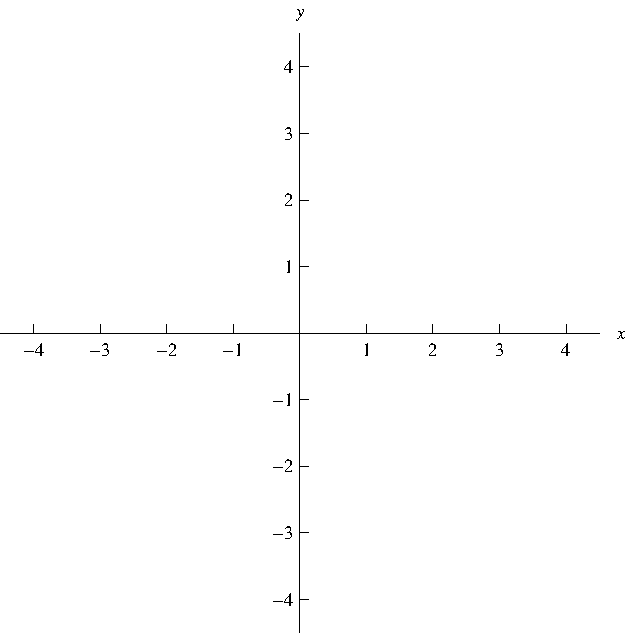
\includegraphics[height=6cm]{parametric-curves/pictures/11-01-ex1a.pdf}%
%}%
%\only<handout:0| 3-4>{%
%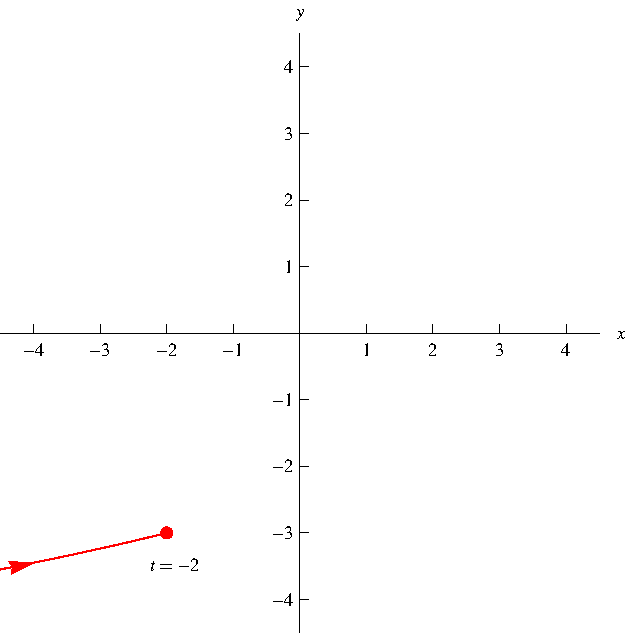
\includegraphics[height=6cm]{parametric-curves/pictures/11-01-ex1b.pdf}%
%}%
%\only<handout:0| 5-6>{%
%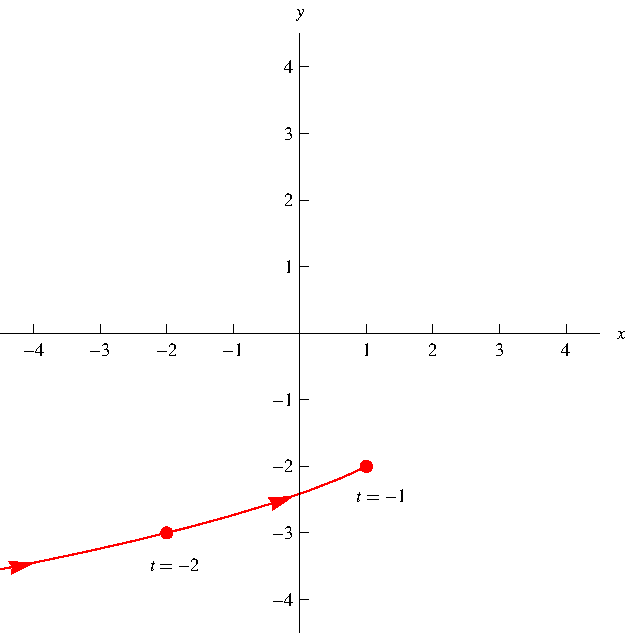
\includegraphics[height=6cm]{parametric-curves/pictures/11-01-ex1c.pdf}%
%}%
%\only<handout:0| 7-8>{%
%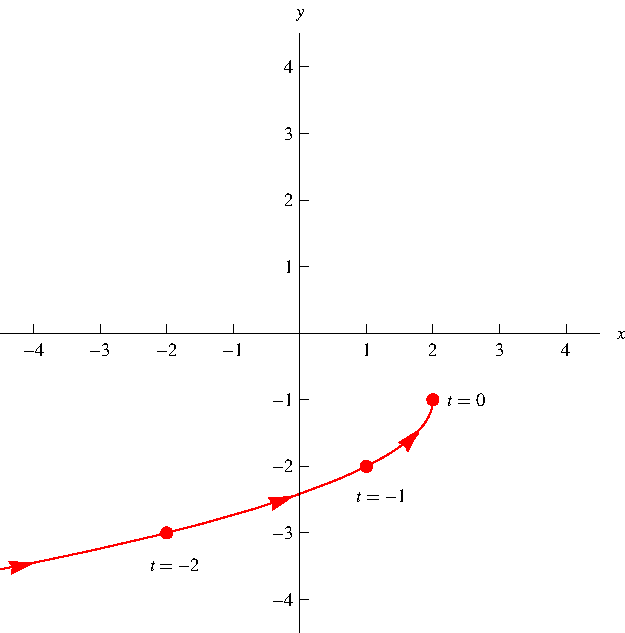
\includegraphics[height=6cm]{parametric-curves/pictures/11-01-ex1d.pdf}%
%}%
%\only<handout:0| 9-10>{%
%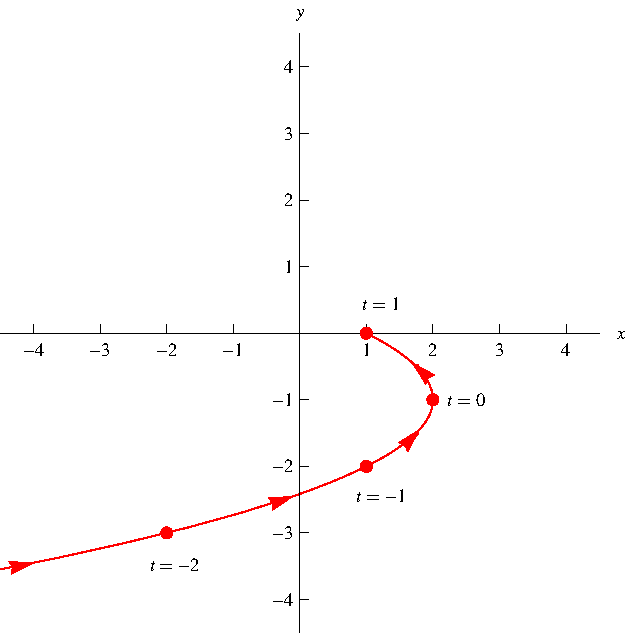
\includegraphics[height=6cm]{parametric-curves/pictures/11-01-ex1e.pdf}%
%}%
%\only<handout:0| 11>{%
%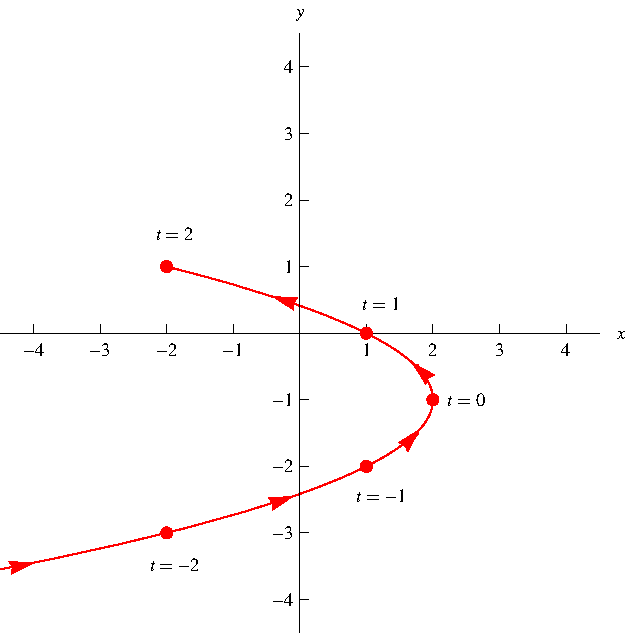
\includegraphics[height=6cm]{parametric-curves/pictures/11-01-ex1f.pdf}%
%}%
%\only<12->{%
%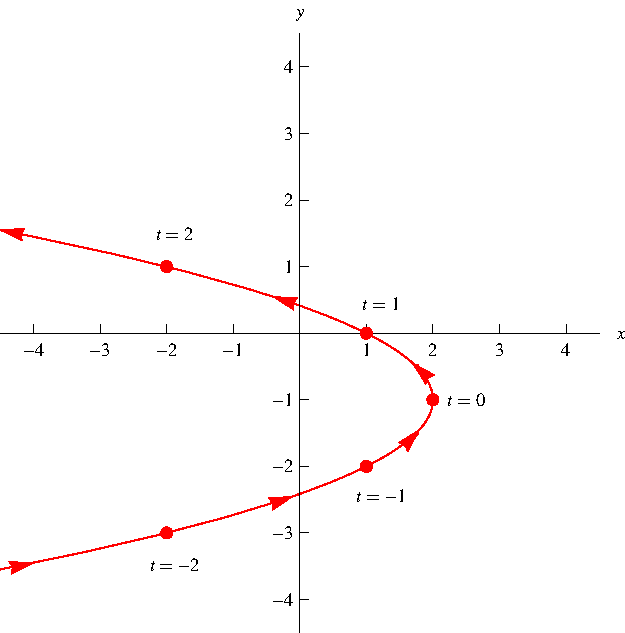
\includegraphics[height=6cm]{parametric-curves/pictures/11-01-ex1g.pdf}%
%}%
\column{.5\textwidth}
\hfil \hfil
$
\begin{array}{|r|r|r|}
\hline
\alert<2,4,6,8,10>{ t} & x & y\\
\hline
\alert<handout:0| 2-3>{-2} &%
\alert<handout:0| 2-3>{\uncover<3->{-2}} &%
\alert<handout:0| 2-3>{\uncover<3->{-3}} \\%
\alert<handout:0| 4-5>{-1} &%
\alert<handout:0| 4-5>{\uncover<5->{1}} &%
\alert<handout:0| 4-5>{\uncover<5->{-2}} \\%
\alert<handout:0| 6-7>{0} &%
\alert<handout:0| 6-7>{\uncover<7->{2}} &%
\alert<handout:0| 6-7>{\uncover<7->{-1}} \\%
\alert<handout:0| 8-9>{1} &%
\alert<handout:0| 8-9>{\uncover<9->{1}} &%
\alert<handout:0| 8-9>{\uncover<9->{0}} \\%
\alert<handout:0| 10-11>{2} &%
\alert<handout:0| 10-11>{\uncover<11->{-2}} &%
\alert<handout:0| 10-11>{\uncover<11->{1}} \\%
\hline
\end{array}
$
\hfil

\uncover<14->{%
\noindent Eliminate $t$: from second equation we have $\alert<handout:0| 14,16>{t = y + 1}$ \uncover<15->{%
and therefore:}  %
}%
$\begin{array}{rcl}
\uncover<15->{%
\alert<handout:0| 15,18>{x}%
}%
&\uncover<15->{\alert<handout:0| 15>{ =}}&%
\uncover<15->{%
\alert<handout:0| 15>{ -\alert<handout:0| 16>{t}^2 + 2}%
}\\%
& \uncover<16->{ = }&%
\uncover<16->{%
 -(\alert<handout:0| 16>{y+1})^2 + 2
}\\%
& \uncover<17->{\alert<handout:0| 18>{ = }}&%
\uncover<17->{%
\alert<handout:0| 18>{-y^2 - 2y + 1}
}%
\end{array}
$

\uncover<18->{Thus our curve image is a parabola, as expected.}
\end{columns}
\end{example}
\end{frame}

\begin{frame}
\begin{columns}[c]
\column{.5\textwidth}
%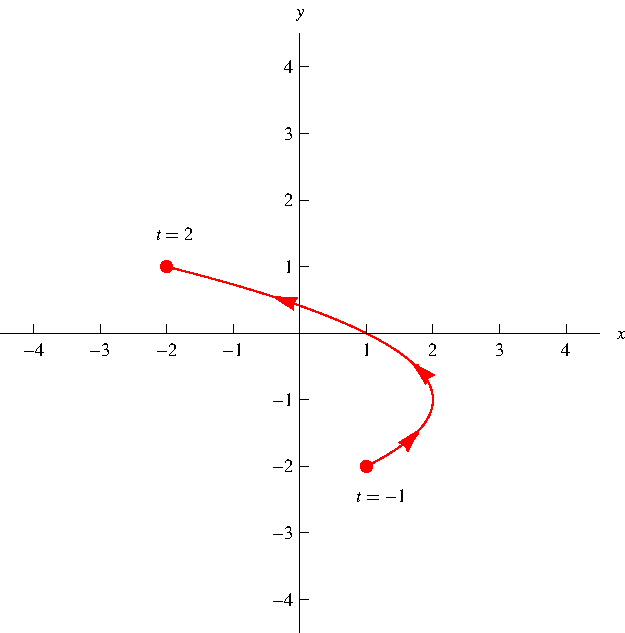
\includegraphics[height=6cm]{parametric-curves/pictures/11-01-ex1chopped.pdf}%
\psset{xunit=0.8cm, yunit=0.8cm}
\begin{pspicture}(-4.5,-4.2)(3.2,2.2)
\psframe*[linecolor=white](-4.5,-4.2)(3.2,2.2)
\tiny
\psaxes[arrows=<->](0,0)(-4.3, -4)(3, 2)
\fcLabels{3}{2}
%Calculator input: plotCurve{}(- t^{2}+2, t-1, -2, 2)

\uncover<1-3>{
\parametricplot[linecolor=\fcColorGraph, arrows=->, plotpoints=150]{ -2.5 }{-1.25}{2 t 2 exp -1 mul add -1 t add }
\parametricplot[linecolor=\fcColorGraph, arrows=->, plotpoints=150]{ -1.25 }{0}{2 t 2 exp -1 mul add -1 t add }
\parametricplot[linecolor=\fcColorGraph, arrows=->, plotpoints=150]{ 0 }{1.25}{2 t 2 exp -1 mul add -1 t add }
\parametricplot[linecolor=\fcColorGraph, plotpoints=150]{ 1.25 }{2.5}{2 t 2 exp -1 mul add -1 t add }
}
\uncover<4->{
\parametricplot[linecolor=\fcColorGraph, plotpoints=150]{ -1 }{0}{2 t 2 exp -1 mul add -1 t add }
\parametricplot[linecolor=\fcColorGraph, arrows=->, plotpoints=150]{ 0 }{1}{2 t 2 exp -1 mul add -1 t add }
\parametricplot[linecolor=\fcColorGraph, plotpoints=150]{ 1 }{2}{2 t 2 exp -1 mul add -1 t add }
}
\uncover<5->{
\fcFullDot{-2}{1}
\fcFullDot{1}{-2}
}
\end{pspicture}
\[
\left|
\begin{array}{rcl}
x & = & -t^2 + 2\\
y & = & t-1
\end{array}
\right.
\uncover<4->{, \alert<handout:0| 4>{-1 \leq t \leq 2}}
\]
\column{.5\textwidth}
\begin{itemize}
\item<1->  There was no restriction placed on $t$ in the last example.
\item<2->  In such a case we assume $t\in (-\infty,\infty)$, i.e., $t$ runs over all real numbers.
\item<3->  In general we are expected to specify the interval in which $t$ lies.
\item<4->  For example, if we restrict the previous example to $t\in [-1,2]$, we get the part of the parabola that begins at $(1,-2)$ and ends at $(-2,1)$.
\item<5->  We say that  $(1,-2)$ is the initial point and $(-2,1)$ is the terminal point of the curve.
\end{itemize}
\end{columns}
\end{frame}
% end module eliminate-parameter-ex



%%begin module area-under-hyperbola-ex1

\begin{frame}
Recall Euler substitution: $x=\frac12\left(\frac{1}{t}- t \right)$, $\alert<2>{\sqrt{x^2+1}=\frac{1}2\left(\frac 1 t +t\right)}$, $\alert<12,13,14>{ t=\sqrt{x^2+1}-x} $, $\alert<3>{ \diff x=-\frac12 \left(\frac1{t^2} +1\right)\diff t}$.
\begin{example}
$
\begin{array}{rcl}
\displaystyle \int \alert<2>{ \sqrt{x^2+1}} \alert<3>{\diff x} \vphantom{ \frac{1}{8}\left(\frac{1}{ (\sqrt{ x^2 +1} -x)^2} - (\sqrt{x^2+1}- x)^2 \right) } &=&
\displaystyle
\only<1-16>{
\uncover<2->{ \alert<3>{-} \int  \alert<2>{\alert<4>{\frac12} \left(\alert<5,6>{\frac1t} +\alert<7,8>{t}\right)} \alert<3>{\alert<4>{ \frac{1}{2}} \left(\alert<5,7>{ \frac 1 {t^2}} +\alert<6,8>{1} \right)\diff t}} \\
\uncover<4->{ &=&\displaystyle -\alert<4>{ \frac 1 4} \alert<9,10,11>{ \int} \left(\alert<5>{ \alert<9>{ \frac{ 1 }{ t^3}}} + \alert<6,7,10>{2\frac{1}t} + \alert<8,11>{t} \right) \alert<9,10,11>{ \diff t} } \\
\uncover<9->{&=&\displaystyle \alert<15>{-\frac{1}4} \left( \alert<9>{ \alert<15>{ -}\frac{ \alert<12>{ t^{-2}}}{\alert<15>{2}}} +\alert<10>{ \alert<15>{2} \ln\alert<14>{ |t|} }+ \alert<11>{\frac{\alert<13>{ t^2}}{\alert<15>{2}}} \right)+C}\\
\uncover<12->{&=&}
}
\uncover<12->{\displaystyle \only<1-24>{  \alert<16,17,18,24>{ \alert<15>{\frac{1}{8}} \left(\frac{1}{\alert<12>{ (\sqrt{ x^2 +1} -x)^2}} - \alert<13>{\left(\sqrt{x^2+1}- x\right)^2} \right) } }}\only<25->{
\alert<25>{ \frac{1}{2}x\sqrt{x^2+1}}
} {~~~~~~~~~~~~~~~~~~~~~~~~~~~~~~~~~~~~~~~~~~~~~~~~~~~~~~}  \\
\uncover<12->{ && \displaystyle \alert<16,17>{ \only<1-30>{\alert<15>{ -}} \only<31->{\alert<31>{+} } \alert<15>{ \frac12}  \alert<26,30>{\ln \left( \alert<14>{ \sqrt{x^2+1} \only<1-30>{-}\only<31->{\alert<31>{+} } x} \right)} +C}}
\end{array}
$

\noindent \only<17-25>{The answer is good. However, let's simplify.

\noindent
\uncover<18->{
$
\begin{array}{l}
\phantom{=}
\displaystyle \alert<18>{ \frac{1}{(\sqrt{x^2+1}-x)^2}- \left( \sqrt{ x^2+1 }-x\right)^2} \\
\uncover<19->{= \displaystyle \frac{ \alert<19>{(\sqrt{x^2+1} +x )^2} }{ ( \sqrt{x^2 +1} -x )^2  	\alert<19>{(\sqrt{x^2+1}+x)^2} } - \left(\sqrt{x^2+1}-x\right)^2} \\
\uncover<20->{ =\displaystyle \frac{(\sqrt{x^2+1}+x)^2}{ \alert<20>{ \alert<21,22>{((\sqrt{x^2 +1 } )^2 -x^2 )^2 } \uncover<21,22>{\alert<21,22>{=1}} } } - \left( \sqrt{x^2 +1 } -x \right)^2} \\
\displaystyle \uncover<22->{=\left(\sqrt{x^2+1}+x\right)^2-\left( \sqrt{ x^2 + 1 } -x\right)^2} \uncover<23->{ = \alert<24,25>{ 4x\sqrt{x^2+1}}}
\end{array}
$
} %uncover<18->
} %only<17-25>

\only<26->{
The last expression can be transformed to:
\[
\begin{array}{rcl}
\displaystyle
\alert<26>{\ln} \left(\frac{\alert<26,28>{\left(\sqrt{x^2+1}-x\right)} \uncover<27->{ \alert<27,28>{\left( \sqrt{x^2+1}+ x \right)} }}{ \uncover<27->{ \alert<27>{ \sqrt{x^2 +1} +x}}} \right)
&=& \displaystyle \uncover<28->{\alert<29>{ \ln \left( \frac{\alert<28>{ 1} }{ \sqrt{x^2+1}+x}\right)} }\\ \uncover<29->{&=&\alert<29,30,31>{ -\ln \left(\sqrt{x^2+1}+x\right)}}
\end{array}
\]
}
\end{example}

\vspace{8cm}
\end{frame}

\begin{frame}
\begin{example}
Find the area locked b-n the hyperbolas $\alert<2,3>{ y=\pm \sqrt{ x^2+1}}$ and $x=\pm 2\sqrt{ 2}$.
\begin{columns}
\column{.5\textwidth}
\psset{xunit=0.7cm, yunit=0.7cm}
\begin{pspicture}(-3.328427, -3)(3.328427,3)
\psframe*[linecolor=white](-3.328427,-3)(3.328427,3)
\tiny
\uncover<31->{
\pscustom*[linecolor=\fcColorAreaUnderGraph]{
\psplot[linecolor=\fcColorGraph, plotpoints = 1000 ] {-2.828427} {2.828427}{1 x 2 exp add 0.5 exp }
\psline[linecolor=\fcColorGraph](2.828427,-3)(2.828427,3)
\psplot[linecolor=\fcColorGraph, plotpoints=1000] { 2.828427 } {-2.828427}{1 x 2 exp add 0.5 exp -1 mul }
\psline[linecolor=\fcColorGraph](-2.828427,-3)(-2.828427,3)
}
}
\uncover<1-26,28->{
\psaxes[arrows=<->,ticks=none, labels=none](0,0)(-3,-3)(3,3)
}
\psline[linecolor=red!1](3.301,2)(3.302,2)
\psline[linecolor=red!1](-3.301,2)(-3.302,2)

%Function formula: - (x^{2}+1)^{1/2}
\psplot[linecolor=\fcColorGraph, plotpoints=1000]{-2.828427}{2.828427}{1 x 2 exp add 0.5 exp -1 mul }
\uncover<3-4>{\rput[tl](-2.2, -2.4){ \alert<3>{ $y= - \sqrt{ x^2 +1 }$}}}

%Function formula: (x^{2}+1)^{1/2}
\psplot[linecolor=\fcColorGraph, plotpoints=1000]{-2.828427}{ 2.828427 }{1 x 2 exp add 0.5 exp }
\uncover<2-4>{\rput[bl](-2.1, 2.4){\alert<2>{ $y=\sqrt{ x^2 +1} $}}}

\uncover<29->{
\psline[linecolor=\fcColorGraph](-2.828427,3)(-2.828427,-3)
}
\uncover<30->{
\psline[linecolor=\fcColorGraph](2.828427,3)(2.828427,-3)
}
\uncover<25-27>{
\psline{<->}(-2.9,2.9)(2.9,-2.9)
\rput[t](-2.1, 1.7){$\begin{array}{l} \alert<25>{v=0} \\\uncover<1-26>{\alert<25>{y+x=0}} \end{array}$}
}
\uncover<15-27>{
\psline{<->}(-2.9,-2.9)(2.9,2.9)
\rput[b](-2.1, -1.9){$\begin{array}{l} \uncover<1-26>{ \alert<15>{ y-x=0 }}\\\uncover<16->{\alert<16>{u=0}} \end{array}$}
}
\uncover<17-26>{
\fcFullDot{1.4}{1.4}
\rput[l]( 1.6, 1.4){$(\frac{y+x}{2},\frac{y+x}{2})$}
}
\uncover<14-26>{
\fcFullDot{0.6}{2.2}
\rput[lb](0.65, 2.2){$(x,y)$}
}
\uncover<26>{
\psline(0.6,2.2)(-0.8,0.8)
\psline(-0.7, 0.9)(-0.6, 0.8)(-0.7, 0.7)
\rput[rb](-0.3, 1.3){\alert<26>{$v$}}
}
\uncover<18-26>{
\psline(0.6,2.2)(1.4, 1.4)
\psline(1.3, 1.5)(1.2,1.4)(1.3, 1.3)
}
\uncover<23-26>{
\rput[tr](0.95, 1.8){\alert<23>{$u$}}
}
\uncover<14-26>{
\fcFullDot{2.2}{0.6}
\rput[lt]( 2.2, 0.65){$(y,x)$}
}
\end{pspicture}

\vbox to 3.0cm {
\uncover<18->{\alert<18>{
\uncover<22->{\alert<22>{Signed}} distance b-n $(x,y)$ and line $u=0$ equals}}
\only<1-23>{
$\uncover<19->{\uncover<22->{\alert<22>{\pm}} \alert<19>{ \sqrt{ \alert<20>{ \left(x-\frac{(x+y)}{2} \right)^2+ \left( y- \frac{(x+y )}{2} \right)^2}}}}
$
$\uncover<20->{=\uncover<22->{\alert<22>{\pm}} \sqrt{ \alert<20>{ \frac{1}{2}(y-x)^2 }}} \uncover<21->{= \alert<21>{ \uncover<1-21>{\pm} \alert<23>{ \frac{\sqrt{2 }}{ 2 } ( y-x)}}} \uncover<23>{ \alert<23>{=}}$
} %only<1-23>
\uncover<23->{ \alert<23,24>{$u $}.}
\only<24->{\uncover<25->{
Similarly compute that \alert<26>{signed distance b-n $(x,y)$ and the \alert<25>{line $v=0$} equals $v$}.
\uncover<27->{$\Rightarrow$ $y^2-x^2=1$ is the \alert<27>{ hyperbola $v=\frac{1/2}{v}$} in the $(u,v)$-plane.}
}}

\vfil
} %vbox

\column {.5\textwidth}
\only<1-27>{
\uncover<4->{We studied $\alert<27>{v=\frac{1/2}{u}}$ is called a hyperbola:}\uncover<3->{ why do we call $y= \sqrt{ x^2 +1}$ hyperbola?} \uncover<5->{Compute:}
\[
\begin{array}{rcl}
\uncover<5->{\sqrt{x^2+1} &=& y}\\
\uncover<6->{ x^2+1 &=& y^2}\\
\uncover<7->{y^2-x^2&=&1}\\
\uncover<8->{\uncover<9>{\alert<9>{\frac{1}{2}}} \uncover<10->{\alert<10,11>{\frac{\sqrt{2}}{2}}} \alert<11>{(y-x)} \uncover<10->{\alert<10,12>{\frac{\sqrt{2}}{2}}} \alert<12>{(y+x)}&=&\uncover<9->{\alert<9>{\frac{1}{2}}} \uncover<8>{1}}\\
\uncover<11->{\alert<11>{u}\alert<12>{v}&=& \frac{1}{2}}\\
\uncover<13->{\alert<27>{v}&\alert<27>{=}& \alert<27>{\frac{1/2}{u}},}
\end{array}
\]
\uncover<11->{where $\begin{array}{|l}
\alert<11,16,23>{u=\frac{\sqrt{2}}{2} \left(y-x\right)}\\
\alert<12,25>{v=\frac{\sqrt{2}}{2}\left(y+x\right)}
\end{array}$. } \uncover<14->{Consider an arbitrary point $(x,y)$.}
} %only<1-27>
\only<28->{
The area in question is:
$
\begin{array}{l}
\displaystyle\phantom{=} \int \limits^{{{\uncover<28,29>{\alert<29>{ \textbf{?}}}\uncover<30->{\alert<30>{ 2\sqrt{2}}}}}}_{\uncover<28>{\alert<28>{\textbf{?}}}\uncover<29->{ -2\sqrt{2}}} 2\sqrt{x^2+1}\diff x \\
\displaystyle \uncover<32->{= \uncover<33->{\alert<33>{2}} \left[x\sqrt{x^2+1} \vphantom{\ln \left(\sqrt{x^2+1}+x\right) }\right.}\\
\displaystyle \uncover<32->{\left. \ln \left(\sqrt{x^2+1}+x\right)\right]^{2\sqrt{2}}_{\only<33->{\alert<33>{0}} \uncover<1-32>{-2\sqrt{2}}}}\\
\uncover<34->{=2\left(2\sqrt{2} \sqrt{(2\sqrt{2})^2+1}\right.} \\
\uncover<34->{\left.+ \ln \left(\sqrt{(2\sqrt{2})^2+1}+2\sqrt{2} \right) \right)}\\
\uncover<35->{=12\sqrt{2} +2\ln \left(3+2\sqrt{2}\right )}\\
\uncover<36->{\approx 20.496}
\end{array}
$
}
\end{columns}

\end{example}

\end{frame}

%end module area-under-hyperbola-ex1


 


\end{document}
